% Trabalho de Oficina de Planejamento e Governança Metropolitana
%
% Abaixo seguem orientações originais do modelo utilizado.
%
% Siga para o conteúdo do trabalho descendo até a linha 908.
%
% ==============================================================
%
% Modelo para monografia de final de curso, em conformidade
% com normas da ABNT implementadas pelo projeto abntex2.
%
% Este arquivo é fortemente baseado em exemplo distribuído no
% mesmo projeto. O projeto abntex2 pode ser acessado pela página
% http://abntex2.googlecode.com/
%
% Este arquivo pode ser rodado tanto com o pdflatex quanto com
% o lualatex.  Como contém referências bibliográficas a serem
% processadas pelo programa bibtex, este programa deve ser
% executado. Em resumo, a ordem de execução deve ser:
% rodar primeiro o pdflatex (ou o lualatex), depois o bibtex e,
% a seguir, o pdflatex (ou o lualatex ) novamente mais duas vezes,
% para assegurar que todas as referências bibliográficas e 
% citações estejam atualizadas.
%
% Para adaptar os textos para uso pessoal, usar os comandos
% imediatamente antes do \begin{document} (iniciando com o
% comando \titulo).  
%
% Este modelo está adaptado para monografias de final de curso
% em matemática da UFRJ, mas, com o uso das variáveis, pode ser
% usado para outros tipos de trabalho (mestrado, doutorado),
% outros cursos, universidades etc.  Caso a adaptação das
% variáveis não seja suficiente, pode-se alterar os comandos
% imprimircapa, imprimirfolhaderosto e imprimiraprovação, 
% fazendo as alterações necessárias.  Como os comandos definidos
% neste texto usam somente LaTeX, a sua adaptação deve ser 
% simples, bastando algum conhecimento de LaTeX.
%
% O restante do preâmbulo provavelmente  não necessitará ser
% alterado, a menos, eventualmente, das opções de chamada da
% classe abntex2, que estão definidas a seguir.
% 
\documentclass[ 
% -- opções da classe memoir que é a classe base da abntex2 --
% tamanho da fonte
12pt,
% capítulos começam em pág ímpar. Insere pág vazia, se preciso
openright,
% para imprimir uma página por folha ou visualização em video 
oneside,
% frente e verso. Margens das pag. ímpares diferem das pares.
%  twoside,
% tamanho do papel. 
a4paper,
% Caio - Ocultando bordas horríveis em hiperligações
hidelinks,
% -- opções da classe abntex2 --
% títulos de capítulos convertidos em letras maiúsculas
%  chapter=TITLE,
% títulos de seções convertidos em letras maiúsculas
%  section=TITLE,
% títulos de subseções convertidos em letras maiúsculas
%  subsection=TITLE,
% títulos de subsubseções convertidos em letras maiúsculas
%  subsubsection=TITLE,
% -- opções do pacote babel --
english,   % idioma adicional para hifenização
portuguese,   % o último idioma é o principal do documento
oldfontcommands,
]{abntex2}
%
% ==============================================================
%
% --------------------------------------------------------------
% Adicionando pacotes para recursos adicionais e defindo opções
% pertinentes
% --------------------------------------------------------------
%
% cabeçalho comum para uso com lualatex ou pdflatex
\usepackage{ifluatex}
% opções para uso com o lualatex
\ifluatex
\usepackage{fontspec}
\defaultfontfeatures{Ligatures=TeX}
% o fonte small caps é diferente no latin modern
\fontspec[SmallCapsFont={Latin Modern Roman Caps}]{Latin Modern Roman}
% pacotes da AMS 
\usepackage{amsmath,amsthm} 
% pacote para fonte específico para símbolos matemáticos
\usepackage{unicode-math}
\setmathfont{Latin Modern Math}
% latin modern tem simbolos de mathbb muito feios.
%  Trocar o fonte para estes simbolos.
\setmathfont[range=\mathbb]{Tex Gyre Pagella Math}
% opções para uso com o pdflatex
\else
\usepackage[utf8x]{inputenc}
\usepackage[T1]{fontenc}
\usepackage{lmodern}
\usepackage{etoolbox}
% pacotes da AMS 
\usepackage{amsmath,amssymb,amsthm} 
% Mapear caracteres especiais no PDF
\usepackage{cmap}
\fi

% pacotes usados tanto pelo lualatex quanto pelo pdflatex
\usepackage{lastpage}    % Usado pela Ficha catalográfica
\usepackage{indentfirst} % Indenta primeiro parágrafo 
\usepackage{color}       % Controle das cores
\usepackage{graphicx}    % Inclusão de gráficos
\usepackage{wrapfig}     % gráficos ao redor do texto
% pacote para ajustar os fontes em cada linha de forma a
% respeitar as margens
\usepackage{microtype}
% permite a gravação de texto em um arquivo indicado a partir
% deste arquivo.  Originalmente foi usado para criar o arquivo
% .bib com conteúdo de exemplo, evitando a edição de um arquivo
% .bib somente para a bibliografia
\usepackage{filecontents}

% Caio - diagramas
% http://www.texample.net/tikz/examples/smart-priority/
%\usepackage{smartdiagram}

% Caio - ladeando imagens
% https://tex.stackexchange.com/questions/57433/cannot-use-caption-under-minipage
\usepackage{caption}

% Caio - preciso de tabelas longas
% http://www.tex.ac.uk/FAQ-figurehere.html
\usepackage{longtable}

% Caio - quero alternar as cores das linhas da tabela
% https://tex.stackexchange.com/questions/107944/alternate-row-colors-in-longtable
\usepackage[table]{xcolor}
\definecolor{lightgray}{gray}{0.9}

% Caio - tentando melhorar o posicionamento das imagens
\usepackage{float}

% Caio - corrigindo espaçamento conforme http://tex.stackexchange.com/questions/5683/how-to-remove-top-and-bottom-whitespace-of-longtable
\setlength{\LTpre}{0pt}
\setlength{\LTpost}{0pt}

% Caio - preciso de plotagens
%\usepackage{pgfplots}
%\pgfplotsset{compat=1.8}

% Caio - quero usar letras nas listas do enumerate conforme https://tex.stackexchange.com/questions/2291/how-do-i-change-the-enumerate-list-format-to-use-letters-instead-of-the-defaul
\usepackage{enumitem}

% Caio - listas de códigos
\usepackage{listings}

\lstset{
	breaklines=true,
	breakatwhitespace=false,
	numbers=left,
	numbersep=5pt,
	numberstyle=\tiny\color{gray}
}

% Caio - modo paisagem para tabelões
\usepackage{lscape}

% Caio - adicionando o pacote hyperref
\usepackage{hyperref}
% - e definindo metadados do PDF e comportamento dos links
\hypersetup{
	%pagebackref=true,
	pdftitle={Produto III}, 
	pdfauthor={Vários},
	pdfsubject={governança metropolitana},
	colorlinks=false,      		% false: boxed links; true: colored links
	linkcolor=blue,          	% color of internal links
	citecolor=blue,        		% color of links to bibliography
	filecolor=magenta,      	% color of file links
	urlcolor=blue,
	bookmarksdepth=4
}

% Caio - separação silábica
%\hyphenation{}

% Caio - citações mais poderosas
%\usepackage[autostyle]{csquotes}

%-----------------------------------------------------------
%-----------------------------------------------------------
% Caio - habilitar glossário
\usepackage{glossaries}
\makeglossaries

% \newglossaryentry{ex}{name={sample},description={an example}}
\newglossaryentry{rmc}{
	name={RMC},
	description={Região Metropolitana de Curitiba}
}

\newglossaryentry{comec}{
	name={COMEC},
	description={Coordenação da Região Metropolitana de Curitiba}
}

\newglossaryentry{ippuc}{
	name={IPPUC},
	description={Instituto de Pesquisa e Planejamento Urbano de Curitiba}
}

\newglossaryentry{fpic}{
	name={FPIC},
	description={Função pública de interesse comum}
}

\newglossaryentry{regic}{
	name={REGIC},
	description={Regiões de Influência das Cidades}
}

\newglossaryentry{rm}{
	name={RM},
	description={Região Metropolitana}
}

\newglossaryentry{rms}{
	name={rms},
	description={Regiões Metropolitanas}
}

\newglossaryentry{ipardes}{
	name={IPARDES},
	description={Instituto Paranaense de Desenvolvimento Econômico e Social}
}

\newglossaryentry{ibge}{
	name={IBGE},
	description={Instituto Brasileiro de Geografia e Estatística}
}

\newglossaryentry{rit}{
	name={RIT},
	description={Rede Integrada de Transporte}
}

\newglossaryentry{nuc}{
	name={NUC},
	description={Núcleo Urbano Central}
}

\newglossaryentry{cic}{
	name={CIC},
	description={Cidade Industrial de Curitiba}
}

\newglossaryentry{ciar}{
	name={CIAR},
	description={Centro Industrial de Araucária}
}

\newglossaryentry{utp}{
	name={UTP},
	description={Unidade Territorial de Planejamento}
}

\newglossaryentry{pib}{
	name={PIB},
	description={Produto Interno Bruto}
}

\newglossaryentry{ipdm}{
	name={IPDM},
	description={Índice de Desempenho Municipal}
}

\newglossaryentry{pdi}{
	name={PDI},
	description={Plano de Desenvolvimento Integrado}
}

\newglossaryentry{dnaee}{
	name={DNAEE},
	description={Departamento Nacional de Água e Energia Elétrica}
}

\newglossaryentry{sanepar}{
	name={SANEPAR},
	description={Companhia de Saneamento do Paraná}
}

\newglossaryentry{agepar}{
	name={AGEPAR},
	description={Agência Reguladora do Paraná}
}

\newglossaryentry{snis}{
	name={SNIS},
	description={Sistema Nacional de Informações sobre Saneamento}
}

\newglossaryentry{rais}{
	name={RAIS},
	description={Relação anual de informações sociais}
}

\newglossaryentry{fjp}{
	name={FJP},
	description={Fundação João Pinheiro}
}

\newglossaryentry{brt}{
	name={BRT},
	description={Bus Rapid Transit}
}

\newglossaryentry{cco}{
	name={CCO},
	description={Centro de Controle Operacional}
}

\newglossaryentry{pnd}{
	name={PND},
	description={Plano Nacional de Desenvolvimento}
}

\newglossaryentry{cdi}{
	name={CDI},
	description={Conselho de Desenvolvimento Industrial}
}

\newglossaryentry{befiex}{
	name={BEFIEX},
	description={Programa de Benefícios Fiscais às Exportações}
}

\newglossaryentry{bndes}{
	name={BNDES},
	description={Banco Nacional de Desenvolvimento Econômico e Social}
}

\newglossaryentry{mnlm}{
	name={MNLM},
	description={Movimento Nacional de Luta pela Moradia}
}

\newglossaryentry{ugb}{
	name={UGB},
	description={Urban Growth Boundary}
}

\newglossaryentry{dlcd}{
	name={DLCD},
	description={Department of Land Conservation and Development}
}

\newglossaryentry{odot}{
	name={ODOT},
	description={Oregon Department of Transportation}
}

\newglossaryentry{tod}{
	name={TOD},
	description={Transit Oriented Development}
}

\newglossaryentry{fgts}{
	name={FGTS},
	description={Fundo de Garantia do Tempo de Serviço}
}

\newglossaryentry{bnh}{
	name={BNH},
	description={Banco Nacional da Habitação}
}

%-----------------------------------------------------------
%-----------------------------------------------------------
% Comandos para definir ambientes tipo teorema em português 
\newtheorem{meuteorema}{Teorema}[chapter]
\newtheorem{meuaxioma}{Axioma}[chapter]
\newtheorem{meucorolario}{Corolário}[chapter]
\newtheorem{meulema}{Lema}[chapter]
\newtheorem{minhaproposicao}{Proposição}[chapter]
\newtheorem{minhadefinicao}{Definição}[chapter]
\newtheorem{meuexemplo}{Exemplo}[chapter]
\newtheorem{minhaobservacao}{Observação}[chapter]
%-----------------------------------------------------------
%-----------------------------------------------------------
% Pacotes de citações
\usepackage[brazilian,hyperpageref]{backref}
\usepackage[alf]{abntex2cite}   % Citações padrão ABNT
%\usepackage[num]{abntex2cite}  % Citações numéricas
% --- 
% Configurações do pacote backref
% Usado sem a opção hyperpageref de backref
\renewcommand{\backrefpagesname}{Citado na(s) página(s):~}
% Texto padrão antes do número das páginas
\renewcommand{\backref}{}
% Define os textos da citação
\renewcommand*{\backrefalt}[4]{
	\ifcase #1 %
	Nenhuma citação no texto.%
	\or
	Citado na página #2.%
	\else
	Citado #1 vezes nas páginas #2.%
	\fi}%
% --- 
% --- 
% Espaço em branco no início do parágrafo
\setlength{\parindent}{1.3cm}
% Controle do espaçamento entre um parágrafo e outro:
\setlength{\parskip}{0.2cm}  % tente também \onelineskip
% ---
% compila o indice, se este for incluído no texto
\makeindex
%
% --------------------------------------------------------- 
% ---------------------------------------------------------
% Redefinindo o comando do abntex2 para gerar uma capa  
\renewcommand{\imprimircapa}{%
	\begin{capa}
		\begin{figure}
			\centering
			
\includegraphics[width=0.3\linewidth]{img/logotipo-ufabc-abaixo}
		\end{figure}	
		\begin{flushleft} 
			{\centering \Large \textsc{\imprimirinstituicao  \\
					\imprimircurso \\} }
		\end{flushleft}
		
		\vfill
		\begin{center}
			{\large \imprimirautor} \\
			\vspace*{0.5cm}
			{\Large \textit{\imprimirtitulo}}
		\end{center}
		
		\vfill
		\begin{center}
			{\large{\imprimirlocal \\ \imprimirano  }}
		\end{center}
		\vspace*{1cm} 
	\end{capa}
	
}

% ---------------------------------------------------------
% ---------------------------------------------------------
%
%
% ---------------------------------------------------------
% ---------------------------------------------------------
% Redefinindo o comando para gerar uma folha de rosto 
\renewcommand{\imprimirfolhaderosto}{%
	\begin{center}
		{\large \imprimirautor}
	\end{center}
	\vfill \vfill \vfill \vfill
	\begin{center}
		{\Large \textit{\imprimirtitulo}}
	\end{center}
	
	\vfill \vfill \vfill 
	\begin{flushright} 
		\parbox{0.5\linewidth}{
			\imprimirtipotrabalho\, relacionado ao 
			\imprimircurso\, da \imprimirsigla\, 
			entregue como parte do
			processo de graduação para a obtenção do 
			grau de \imprimirgrau.}
	\end{flushright} 
	
	\vfill 
	\begin{flushright} 
		\parbox{0.5\linewidth}{ \imprimirorientadorRotulo 
			\imprimirorientador\\ \imprimirttorientador}
	\end{flushright} 
	
	\ifdefvoid{\imprimircoorientador}{}{
		\begin{flushright} 
			\parbox{0.5\linewidth}{ \imprimircoorientadorRotulo 
				\imprimircoorientador\\ \imprimirttcoorientador}
		\end{flushright}
	}
	
	\vfill \vfill \vfill \vfill \vfill \vfill \vfill
	\begin{center}
		{\large{\imprimirlocal \\ \imprimirano}}
	\end{center}
	\vspace*{1cm} \newpage
}
% Final do comando para gerar uma folha de rosto 
% ---------------------------------------------------------
% ---------------------------------------------------------
%
%
% ---------------------------------------------------------
% ---------------------------------------------------------
% Definindo o comando para gerar uma folha de defesa 
\newcommand{\imprimirfolhadeaprovacao}{%
	\begin{center}
		{\large \imprimirautor}
	\end{center}
	\vfill \vfill \vfill \vfill
	\begin{center}
		{\Large \textit{\imprimirtitulo}}
	\end{center}
	
	\vfill \vfill \vfill \vfill \vfill \vfill
	\begin{flushright} 
		\parbox{0.5\linewidth}{
			%			\imprimirtipotrabalho\,apresentada ao 
			%			\imprimircurso\, da \imprimirsigla\, como requisito
			%			para a obtenção parcial do grau de \imprimirgrau.}
		}
	\end{flushright} 
	\vfill \vfill \vfill \vfill
	Aprovada em \data.
	
	\vfill \vfill \vfill \vfill
	
	\begin{center}
		\textbf{BANCA EXAMINADORA}
		
		\vfill\vfill\vfill
		\rule{10cm}{.1pt}\\
		{\imprimirexaminadorum} \\ {\imprimirttexaminadorum}
		
		\ifdefvoid{\imprimirexaminadordois}{}{
			\vfill\vfill
			\rule{10cm}{.1pt}\\
			\imprimirexaminadordois \\ \imprimirttexaminadordois }
		
		\ifdefvoid{\imprimirexaminadortres}{}{
			\vfill\vfill
			\rule{10cm}{.1pt}\\
			\imprimirexaminadortres \\ \imprimirttexaminadortres }
		
		\ifdefvoid{\imprimirexaminadorquatro}{}{
			\vfill\vfill
			\rule{10cm}{.1pt}\\
			\imprimirexaminadorquatro \\ \imprimirttexaminadorquatro }
	\end{center}
	
	\vfill \vfill 
	\begin{center}
		{\large{\imprimirlocal \\ \imprimirano}}
	\end{center}
	\vspace*{1cm}
	\newpage
}
% Final do comando para gerar uma folha de defesa 
% ---------------------------------------------------------
% --------------------------------------------------------
%
%
%
%
%
% ---------------------------------------------------------
% --------------------------------------------------------
% definindo variáveis adicionais 
\providecommand{\imprimirsigla}{}
\newcommand{\sigla}[1]{\renewcommand{\imprimirsigla}{#1}}
%
\providecommand{\imprimircurso}{}
\newcommand{\curso}[1]{\renewcommand{\imprimircurso}{#1}}
%
\providecommand{\imprimirano}{}
\newcommand{\ano}[1]{\renewcommand{\imprimirano}{#1}}
%
\providecommand{\imprimirgrau}{}
\newcommand{\grau}[1]{\renewcommand{\imprimirgrau}{#1}}
%
\providecommand{\imprimirexaminadorum}{}
\newcommand{\examinadorum}[1]{
	\renewcommand{\imprimirexaminadorum}{#1}}
%
\providecommand{\imprimirexaminadordois}{}
\newcommand{\examinadordois}[1]{
	\renewcommand{\imprimirexaminadordois}{#1}}
%
\providecommand{\imprimirexaminadortres}{}
\newcommand{\examinadortres}[1]{
	\renewcommand{\imprimirexaminadortres}{#1}}
%
\providecommand{\imprimirexaminadorquatro}{}
\newcommand{\examinadorquatro}[1]{
	\renewcommand{\imprimirexaminadorquatro}{#1}}
%
\providecommand{\imprimirttorientador}{}
\newcommand{\ttorientador}[1]{
	\renewcommand{\imprimirttorientador}{#1}} 
%
\providecommand{\imprimirttcoorientador}{}
\newcommand{\ttcoorientador}[1]{
	\renewcommand{\imprimirttcoorientador}{#1}}
%
\providecommand{\imprimirttexaminadorum}{}
\newcommand{\ttexaminadorum}[1]{
	\renewcommand{\imprimirttexaminadorum}{#1}}
%
\providecommand{\imprimirttexaminadordois}{}
\newcommand{\ttexaminadordois}[1]{\renewcommand{
		\imprimirttexaminadordois}{#1}}
%
\providecommand{\imprimirttexaminadortres}{}
\newcommand{\ttexaminadortres}[1]{
	\renewcommand{\imprimirttexaminadortres}{#1}}
%
\providecommand{\imprimirttexaminadorquatro}{}
\newcommand{\ttexaminadorquatro}[1]{
	\renewcommand{\imprimirttexaminadorquatro}{#1}}
% fim da definição de variáveis adicionais
% ---------------------------------------------------------
% ---------------------------------------------------------
%
% ---
% ---
% ---
% ---
% ---
% ---
% ---
% ---
% ---
% Informações de dados para CAPA, FOLHA DE ROSTO e FOLHA DE DEFESA
%
%----------------- Título e Dados do Autor -----------------
\titulo{Caderno de Sustentação}
\autor{Caio César C. Ortega \and Gustavo Lopes Alcantara \and Mariana Lins Sartori \and Michele Almeida
}
%

%----------Informações sobre a Instituição e curso -----------------
\instituicao{Universidade Federal do ABC \\
	Centro de Engenharia, Modelagem e Ciências Sociais Aplicadas}
%
\sigla{UFABC}
%
\curso{Bacharelado em Planejamento Territorial}
%\curso{Curso de Licenciatura em Matemática}
%\curso{Mestrado em Ensino de Matemática}
%\curso{Doutorado em Matemática}
%
\local{São Bernardo do Campo, SP}
%
%
% -------- Informações sobre o tipo de documento
\tipotrabalho{Relatório}
%\tipotrabalho{Monografia de final de curso}
%\tipotrabalho{Dissertação de mestrado}
%\tipotrabalho{Tese de doutorado}
%
\grau{BACHAREL em Planejamento Territorial}
%\grau{LICENCIADO em Matemática}
%\grau{MESTRE em Matemática}
%\grau{DOUTOR em Ciências}
%
\ano{2019}
\data{Dezembro de 2019} % data da aprovação
%
%------Nomes do Orientador, examinadores.  
\orientador{Prof. Dr. Jeroen Klink}
%\coorientador{Antonio da Silva} % opcional
\examinadorum{Profa. Dra. Silvana Zioni}
\examinadordois{Prof. Dr. Jeroen Klink}
%\examinadortres{Jeferson Leandro Garcia de Araújo}
%\examinadorquatro{Antonio da Silva}
%
%--------- Títulos do Orientador e examinadores ----
%\ttorientador{Bacharel em Física - UEFS}
%\ttcoorientador{Doutor em Matemática - UFRJ} 
%\ttexaminadorum{Doutor em Matemática - UFRJ}
%\ttexaminadordois{Doutor em Matemática - UFRJ}
%\ttexaminadortres{Doutor em Matemática - UFRJ}
%\ttexaminadorquatro{Doutor em Matemática - UFRJ}
%
% ---
% ---
\begin{document}
	
	% ---
	% Chamando o comando para imprimir a capa
	\imprimircapa
	% ---
	% ---
	% Chamando o comando para imprimir a folha de rosto
	%\imprimirfolhaderosto
	% ---
	% ---
	% Chamando o comando para imprimir a folha de aprovação
	%\imprimirfolhadeaprovacao
	% ---
	% ---
	% Dedicatória
	% ---
	%	\begin{dedicatoria}
	%  	 \vspace*{\fill}
	%  	 \centering
	%  	 \noindent
	%  	 \textit{ Este trabalho é dedicado a todos que, com entusiasmo,\\
	%  	 		sonham e lutam por XYZ no ABCDEFG\\
	%  			do XPTO.} \vspace*{\fill}
	%	\end{dedicatoria}
	%	
	%	
	%	\begin{agradecimentos}
	%	Orientação do modelo: insira aqui um parágrafo
	%	\end{agradecimentos}
	%	
	%	
	%
	%---------------------- EPÍGRAFE I (OPCIONAL)--------------
	%\begin{epigrafe}
	%    \vspace*{\fill}
	%    \begin{flushright}
	%        \textit{''Texto''\\
	%        Autor}
	%    \end{flushright}
	%\end{epigrafe}
	%
	%
	%
	%--------Digite aqui o seu resumo em %Português--------------
	%\begin{resumo}
	%   Descrição. 
	%
	%   \vspace{\onelineskip}
	%   \noindent
	%   \textbf{Palavras-chaves}: Palavras.
	%\end{resumo}
	
	
	%
	% --- resumo em inglês (abstract) ---
	%\begin{resumo}[Abstract]
	%   \begin{otherlanguage*}{english}
	%      Description.
	%
	%      \vspace{\onelineskip}
	%      \noindent
	%      \textbf{Keywords}: Words.
	%   \end{otherlanguage*}
	%\end{resumo}
	
	%
	%----Sumário, lista de figuras e lista de tabelas ------------
	\tableofcontents 
	\newpage \listoffigures
	\newpage \listoftables
	%---------------------
	%--------------Início do Conteúdo---------------------------
	% o comando textual é obrigatório e marca o ponto onde começa 
	% a imprimir o número da página
	\textual
	%
	%---------------------
	%
	
	
	%
	% O conteúdo começa pra valer a seguir
	%
	
	%
	%===============================================================================
	%
	
	\chapter{Diagnóstico}
	
	\section{Contextualização}
	
	A \glsdesc{rmc} (\gls{rmc}) foi criada pela Lei Complementar  nº 14, de 8 de junho de 1973, que instituiu as primeiras Regiões Metropolitanas brasileiras, sendo elas: São Paulo, Belo Horizonte, Porto Alegre, Recife, Salvador, Curitiba, Belém e Fortaleza. Primeiramente, a RMC era composta por quatorze municípios: Almirante Tamandaré, Araucária, Balsa Nova, Bocaiúva do Sul, Campina Grande do Sul, Campo Largo, Colombo, Contenda, Curitiba, Mandirituba, Piraquara, Quatro Barras, Rio Branco do Sul e São José dos Pinhais. Contudo, após o marco da Constituição Federal de 1988 (CF/1998), a competência de criação e gerenciamento das RMs passa a ser do Estado. Dessa forma, foram adicionados mais quinze municípios, destes, cinco são frutos de desmembramentos (Campo Magro, Tunas do Paraná, Fazenda Rio Grande, Pinhais e Itaperuçu) e dez de legislações estaduais (Adrianópolis, Agudos do Sul, Campo do Tenente, Cerro Azul, Doutor Ulysses, Lapa, Piên, Quitandinha, Rio Negro e Tijucas do Sul).
	
	\subsection{Breves notas sobre a revisão bibliográfica}
	
	As diversas publicações sobre a \gls{rmc} indicam que ela cresceu demasiadamente nas últimas décadas, concentrando a maioria da população e da riqueza do estado do Paraná, isso se deve ao fato de três municípios com os maiores PIBs do Estado estarem na \gls{rmc}, e estes três também figuram como as três cidades paranaenses entre os cinquenta maiores PIBs municipais do país: Curitiba, 4o lugar, polo industrial de comércio e serviços; São José dos Pinhais, 37º. lugar, polo automotivo e sede do aeroporto internacional de Curitiba; e Araucária, 40º. lugar, polo petroquímico e industrial –, possuindo um PIB per capita superior à média nacional, regional (Sul) e estadual. Sua importância econômica acentua o fato de que a rede urbana paranaense, assim como a sulina, concentra os fluxos por atividades de maior complexidade, para um pequeno número de centros que se constituem como polos, demonstrando a seletividade dos lugares com tendência concentradora (IPEA).
	%TODO corrigir IPEA acima, referência insatisfatória
	
	Porém os desafios da \gls{rmc} são imensos, devido ao fato de que, no passado, o município de Curitiba concentrou todo tipo de investimento em detrimento ao resto da região, e ele não planejava com nenhum viés metropolitano, abstendo apenas a focar em medidas apenas locais. em 1965 é criado o \glsdesc{ippuc}, o \gls{ippuc}, que  visava o planejamento em Curitiba, já que era a cidade mais rica e importante do Estado, e só no ano de 1974, como decorrência direta das instruções contidas na Lei Complementar nº 14. o Governo do Estado do Paraná, através de Lei Estadual nº. 6.517, criou a \glsdesc{comec}, \gls{comec}, porém, por Curitiba ser um polo muito forte, a \gls{comec} não conseguiu ter o real impacto que precisava, e o planejamento continuou a ter concentrado no município que dá nome à RM, somente com a entrada das montadoras na região, que vão se instalar nas cidades vizinhas de Curitiba é que ela vai perder um pouco do seu tão grandioso protagonismo, mas nada que mudasse tanto as estruturas. 

	\subsection{Histórico da Região Metropolitana de Curitiba}
	% tópico escrito por Caio
	
	O surgimento da \glsdesc{rmc} se dá no bojo da ditadura militar, sendo realizado pela mesma lei complementar que deu providências para a criação de outras novas regiões metropolitanas brasileiras:
	
	\begin{citacao}
		``Em  1973  foi  aprovada  a  Lei  Complementar  nº  14  que  criou  9  regiões metropolitanas no Brasil, dentre elas a de Curitiba. A RMC, então criada, contava com 14 municípios caracterizados principalmente pela proximidade ao município pólo.'' \apud[p. 53]{ipea2001a}{castro2005a}
	\end{citacao}
	
	Conforme \citeonline{comec2019a}, originalmente a Região Metropolitana de Curitiba, quando de sua formação, disciplina pela Lei Complementar Federal n.º 14/73, abrangia os municípios de Curitiba, Almirante Tamandaré, Araucária, Balsa Nova, Bocaiúva do Sul, Campina Grande do Sul, Campo Largo, Colombo, Contenda, Mandirituba, Piraquara, Quatro Barras, Rio Branco do Sul e São José dos Pinhais, totalizando portanto 14 municípios. A década de 1990, marcada por desmembramentos de municípios, altera as feições dos limites políticos administrativos da região, sendo os novos municípios fruto de desmembramento:
	
	\begin{itemize}
		\item Fazenda Rio Grande, desmembrado de Mandirituba em 28/01/1990;
		\item Tunas do Paraná, desmembrado de Bocaiúva do Sul em 30/04/1990;
		\item Itaperuçu, desmembrado de Rio Branco do Sul em 09/11/1990; e
		\item Pinhais, desmembrado de Piraquara em 18/03/1992.
	\end{itemize}
	
	Assim, até meados da década de 1990, os limites alterados só resultaram na reconfiguração interna da Região Metropolitana de Curitiba, situação que sofreria alteração dois anos após o surgimento de Pinhais. Em 1994 a Lei Estadual n.º 11.027 disciplinou a inclusão dos municípios de Cerro Azul, Doutor Ulysses (desmembrado de Cerro Azul em 20/11/1990), Quitandinha (desmembrado de Contenda e de Rio Negro em 13/06/1961), e Tijucas do Sul; em 1995 a Lei Estadual n.º 11.096 disciplinou a inclusão de Adrianópolis (desmembrado em 25/07/ 1960 de Bocaiúva do Sul), além disso, naquele ano Campo Magro também passou a integrar a região metropolitana (uma vez que fora desmembrado em 11/12/1995 de Almirante Tamandaré); finalmente, na década de 1990, no ano de 1998, por meio da Lei Estadual n.º 12.125, ocorreu a inclusão de Agudos do Sul (desmembrado de Tijucas do Sul em 25/07/1960). A Região Metropolitana de Curitiba encerra a década de 1990 com 25 municípios ante os 14 originais. Como aponta \apudonline[p. 54]{ipea2001a}{castro2005a}, a população da região metropolitana então ultrapassava 2 milhões de habitantes (taxa de crescimento demográfico de 3,22\%).
	
	Na década de 2000, os anos de 2002 e 2011 também são marcados por leis estaduais que disciplinam a inclusão de mais municípios, alterando os limites externos da região: em 2002 a Lei Estadual n.º 13.512 adiciona o município da Lapa; em 2011 a Lei Complementar Estadual n.º 139 adiciona outros três municípios, Campo do Tenente, Piên e Rio Negro.
	
	A \autoref{fig:comec2019a01} permite acompanhar cartograficamente a evolução dos limites internos e externos da \glsdesc{rmc}.
	
	\begin{figure}
		\centering
		\caption{Espacialização da formação histórica da \glsdesc{rmc}, 1974-2002}
		\label{fig:comec2019a01}
		\includegraphics[width=0.7\linewidth]{img/comec2019a_01}
		\legend{Fonte: \citeonline{comec2019a}}
	\end{figure}
	
	\subsection{Metropolização a luz da Constituição Federal de 1988}
	% tópico escrito por Caio
	
	Como apontado por \citeonline[p. 100]{guia2015a}, a autonomia municipal, por ter sido cerceada durante um longo período em decorrência da ditadura militar, ganha força com a Constituição Federal de 1988. O marco da nova Constituição é especialmente importante, pois as insatisfações ``induzem a uma resistência explícita à questão metropolitana, manifesta não só entre os representantes do poder público municipal, como também entre os juristas, parlamentares e estudiosos em geral, afetos a questões urbanas'', em outras palavras, é chegado o momento no qual a palavra de ordem é a municipalização, devido ao neolocalismo que pretendia resgatar significativamente não só sua autonomia, mas também capacidade de investimento.
	
	Como sublinham \citeonline[p. 101]{guia2015a}, ``é fundamental destacar que a questão metropolitana não era vista como prioritária pela Assembléia Nacional Constituinte'', uma vez que esta remetia à noção do esvaziamento dos municípios, bem como ``ranços anteriores do período militar'' \citeonline[p. 101]{guia2015a}, o que produziu um tratamento genérico à questão metropolitana, delegando-a aos estados, por meio do artigo 25. A transferência da responsabilidade para os estados, na altura, não foi tratada com entusiasmo, de forma que apenas Amazonas, Goiás, São Paulo e Santa Catarina estabeleceram critérios que deveriam ser considerados na criação de novas regiões metropolitanas e, ainda assim, o fizeram cuidadosamente, buscando distância do formato de gestão metropolitana autoritário que vigorou durante a ditadura, com os estados da Paraíba, do Maranhão, do Espírito Santo e do Rio Grande do Sul estabelecendo mecanismos de consulta aos municípios e/ou suas populações \cite[p. 102]{guia2015a}.
	
	Em outro extremo, as \gls{fpic}s evoluíram timidamente nas Constituições estaduais:
	
	\begin{citacao}
		``Ressalte-se que apenas um número reduzido de Constituições estaduais avançou na definição das “funções de interesses comuns” dos municípios pertencentes às regiões metropolitanas, sendo o `transporte urbano e sistema viário' a função mais freqüente.'' \cite[p. 102]{guia2015a}
	\end{citacao}

	Apenas as constituições dos estados de São Paulo e do Ceará admitiram a necessidade de ação conjunta entre os entes envolvidos, entretanto, a noção não foi acompanhada de instrumentos claros de repasses e compensações financeiras de algum tipo, problema este que também afetou outras Constituições estaduais. A Constituição Federal de 1988 não estabeleceu diretrizes que pudessem orientar os estados. Para \citeonline[p, 101]{guia2015a}, a equação da política exerceu forte pressão na desidratação das agências metropolitanas:
	
	\begin{citacao}
		``Acredita-se que, nesse aspecto, o centro dos problemas enfrentados encontra-se na definição de critérios para o rateio das despesas e dos investimentos, questão diretamente vinculada à relação entre a cidade-pólo e os demais municípios que integram a região. Na ausência de regras claras, os municípios maiores de cada região metropolitana, bem como os governos estaduais, quase sempre resistem à regulamentação de instrumentos e mecanismos concretos de repasse de recursos para as agências metropolitanas, uma vez que temem aportar maior volume dos recursos sem necessariamente uma contrapartida proporcional no que respeita ao processo de tomada de decisão quanto à alocação desses recursos. Em uma situação como essa, os pressupostos elementares da lógica da ação coletiva indicam que o comportamento dos estados e dos municípios de maior peso não chega a surpreender, já que os custos financeiros seriam, via de regra, maiores do que os possíveis retornos políticos auferidos.''
	\end{citacao}

	\section{Machine Learning no processo de diagnóstico da RMC} \label{sec:machine}
	% feito pela Mari, totalmente responsável pela metodologia e adoção da técnica
	
	\subsection{Machine Learning}
	
	O \textit{Machine Learning} é uma sub-área de inteligência artificial, na qual o termo se refere à capacidade dos sistemas de computação de encontrar soluções para problemas de forma independente, reconhecendo padrões nos bancos de dados \cite{jordan2015a}. Em outras palavras: o Machine Learning permite que os sistemas de TI reconheçam padrões com base nos algoritmos e conjuntos de dados existentes, e desenvolvam conceitos e soluções adequadas com sem depender do \textit{input} e, logo, da subjetividade humana. 
	
	A autonomia e imparcialidade dos resultados trazidos pelo Machine Learning, assim como sua praticidade, são, segundo \citeonline{jordan2015a}, alguns dos principais pontos que fizeram com que este modelo de trabalho evoluísse tanto nas últimas duas décadas. 
	
	Entretanto, o fator decisivo para que essa técnica fosse tão trabalhada, incentivada e investida, é devido a quantidade de aplicações e campos que ela abrange, desde os mais ligados ao seu próprio setor de tecnologia como reconhecimento de objetos e linguagem natural em robôs, até aplicações em medicina, segurança, \textit{banking} e ciências sociais.
	
	\begin{citacao}
		``Many developers of AI systems now recognize that, for many applications, it can be far easier to train a system by showing it examples of desired input-output behavior than to program it manually by anticipating the desired response for all possible inputs. The effect of machine learning has also been felt broadly across computer science and across a range of industries concerned with data-intensive issues, such as consumer services, the diagnosis of faults in complex systems, and the control of logistics chains.'' \cite[p. 255]{jordan2015a}
	\end{citacao}

	Neste trabalho, buscamos explorar as vantagens do Machine Learning para obter mais insumos no momento de definição e diagnóstico do espaço geográfico da \glsdesc{rmc}, de uma ótica mais quantitativa.
	
	\subsection{K-Means}
	
	O \textit{K-Means} é uma técnica de Machine Learning de clusterização (``\textit{clustering}'') utilizada em diversas áreas, baseada na distância matricial euclidiana entre pontos de dados \cite{hartigan1979a}. Seu objetivo é agrupar pontos de dados semelhantes e descobrir padrões subjacentes, sem que qualquer resposta esperada seja previamente declarada.
	
	Operacionalmente, o algoritmo inicia sua tentativa de agrupamento de semelhantes com $k$ grupos iniciais (``\textit{seeds}''). Cada dado plotado na matriz tem sua distância euclidiana comparada com um dos $k$ grupos iniciais e é associado ao de menor erro. Esse processo é repetido inúmeras vezes, sendo em que cada uma delas os $k$ grupos são deslocadas para minimizar a distância/erro entre os dados a serem agrupados, até que sua posição seja otimizada e definida. 

	\begin{figure}
		\centering
		\caption{Representação de operacionalização do K-Means}
		\label{fig:kmeans}
		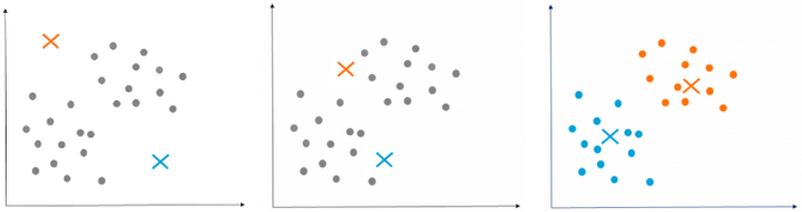
\includegraphics[width=1\linewidth]{img/machine_A}
		\legend{Fonte: \citeonline{santana2017a}}
	\end{figure}

	\subsection{Aplicação do K-Means na \gls{rmc}}
	
	Para a aplicação da técnica K-Means neste trabalho, foi utilizada a sintaxe de programação Python por meio do software Jupyter Notebook. Todo o código desenvolvido encontra-se no \autoref{ap:jupyter} deste documento
	
	\subsubsection{Público}
	
	Como o objetivo deste modelo estatístico era ajudar no diagnóstico da \glsdesc{rmc}, a granularidade do público considerada, ou seja, os pontos a serem plotados na matriz e clusterizados/agrupados, foram todas as 29 cidades que compõe atualmente a \gls{rmc}.
	
	\subsubsection{Variáveis}
	
	As variáveis utilizadas no desenvolvimento do modelo foram extraídas das seguintes fontes:
	
	\begin{itemize}
		\item \gls{ipardes} - \glsdesc{ipardes}
		\item \gls{ibge} - \glsdesc{ibge}
		\item \gls{rais} - \glsdesc{rais}
		\item \gls{fjp} - \glsdesc{fjp}
		\item \gls{snis} - \glsdesc{snis}
		\item \gls{sanepar} - \glsdesc{sanepar}
	\end{itemize}

	Para processo de seleção, foram retiradas variáveis com altos níveis de correlação para não enviesar o resultado. 
	
	Por fim, foram mantidas 107 variáveis. Através delas, buscamos representar ao máximo todas as esferas possíveis de cada uma das cidades como emprego, renda, mobilidade, saneamento, qualidade de vida, evolução populacional, etc, para ter um bom diagnóstico da situação. Importante ressaltar que não foram utilizadas variáveis cartográficas propositalmente, para não enviesar o modelo a criar clusters por distâncias absolutas entre cidades.
	
	\subsubsection{Resultado do processo}
	
	O algoritmo K-Means gerou um bom resultado utilizando-se de 5 clusters, segundo o \textit{output} representado pela \autoref{fig:kmeansoutput}:
	
	\begin{figure}
		\centering
		\caption{Output K-Means Jupyter Notebook}
		\label{fig:kmeansoutput}
		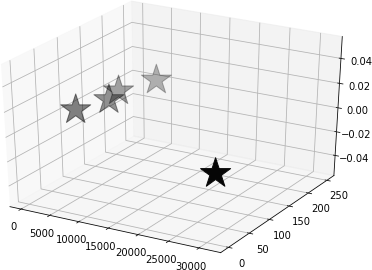
\includegraphics[width=0.5\linewidth]{img/machine_B}
		\legend{Elaboração própria}
	\end{figure}

	É possível notar que um dos clusters destaca-se dos outros (estrela preta) em relação à distância dentro da matriz. Este cluster é composto de uma única cidade: Curitiba, capital da RMC. Este resultado não é inesperado, e representa a disparidade entre a maioria dos dados coletados entre a capital e outras cidades que integram a região metropolitana.
	
	Dos outros quatro grupos formados, podemos notar que os dois pontos no centro da matriz estão sobrepostos. Em análise analítica, pudemos constatar que estes clusters não possuem distância significativa de centroide e por isto, para este exercício, serão agrupados e considerados como um só.
	
	Aplicando o resultado no mapa, temos a \autoref{fig:rmcclusters}.
	
	\begin{landscape}
		\begin{figure}
			\centering
			\caption{Agrupamento dos municípios da \glsdesc{rmc} por similaridade}
			\label{fig:rmcclusters}
			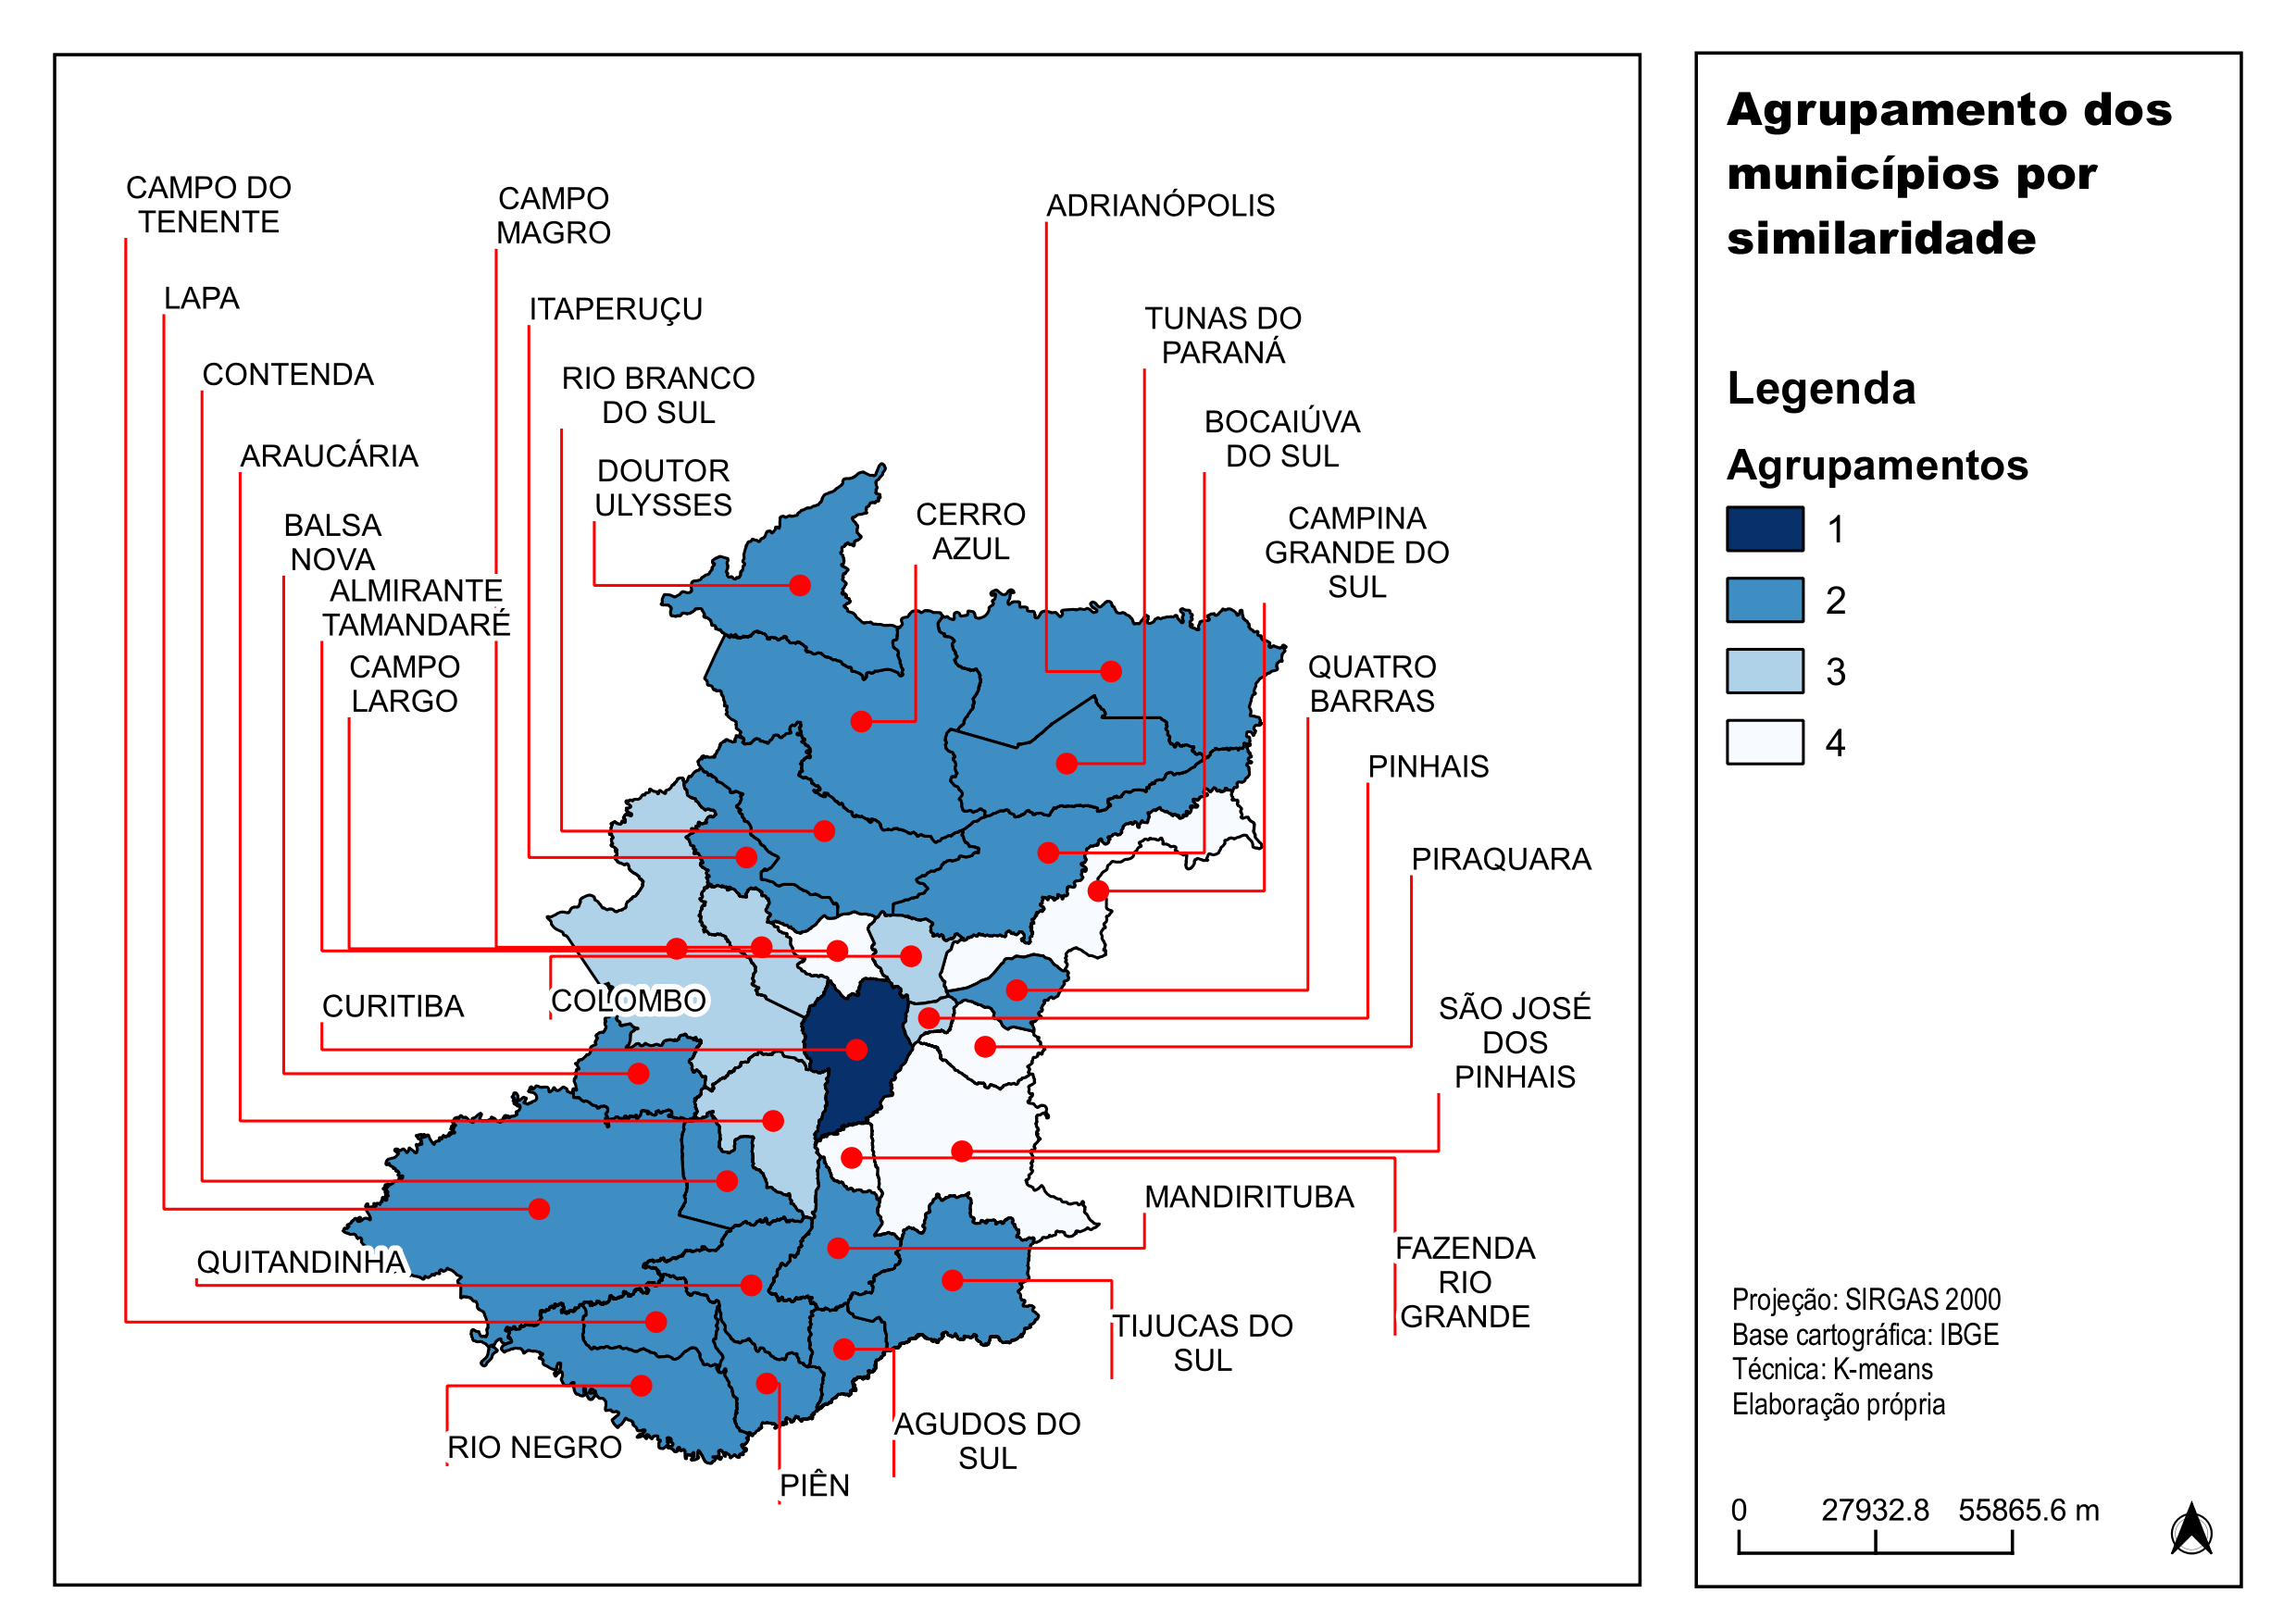
\includegraphics[width=0.85\linewidth]{../gis/produtos/RMC_clusters}
			\legend{Elaboração própria}
		\end{figure}
	\end{landscape}

	A partir do mapa da \autoref{fig:rmcclusters}, é claro notar que a clusterização resultou em um diagnóstico já esperado, em que as cidades do extremo norte e sul, ou seja, que as cidades fora do núcleo urbano formam um único cluster devido as similaridades entre si, e diferenças em relação as cidades mais centrais. O ponto inesperado foi a  cidade de Quatro Barras que, apesar de estar em localização mais central, foi classificada junto às extremidades.
	
	Os clusters intermediários geraram o seguinte agrupamento:
	
	\begin{itemize}
		\item Cluster azul claro (3): Araucária, Colombo, Campo Magro, Campo Largo e Pinhais;
		\item Cluster branco (4): Almirante Tamandaré, Campina Grande do Sul, Piraraquara, São José dos Pinhais, Fazenda Rio Grande.
	\end{itemize}
	
	Por fim, como já citado, Curitiba possui seu próprio cluster devido à disparidade de suas características em relação aos demais municípios.
	
	Em conclusão, a aplicação do método de Machine Learning K-Means para diagnóstico da \gls{rmc} se provou eficaz. O resultado deste modelo estatístico serviu como um dos principais insumos de informação para a recomendação de trabalho que traremos no decorrer deste texto, já a partir da seção seguinte (\autoref{sec:carac}).
	
	\section{Características da região} \label{sec:carac}
	
	Atualmente, a Região Metropolitana de Curitiba possui a maior extensão entre as RMs brasileiras apontadas pelo estudo \gls{regic} \cite{regic2008a}, abrangendo uma área de 16.627 km², o equivalente a 8\% do território do Paraná e população estimada de 3.285.251, em 2012 (Ipardes, 2013a), correspondente a 31\% da população estadual. A \autoref{fig:rmcconfigatual} espacializa a atual configuração da \gls{rmc} a partir de dados do \gls{ibge}.
	
	\begin{landscape}
		\begin{figure}
			\centering
			\caption{Municípios da \glsdesc{rmc}}
			\label{fig:rmcconfigatual}
			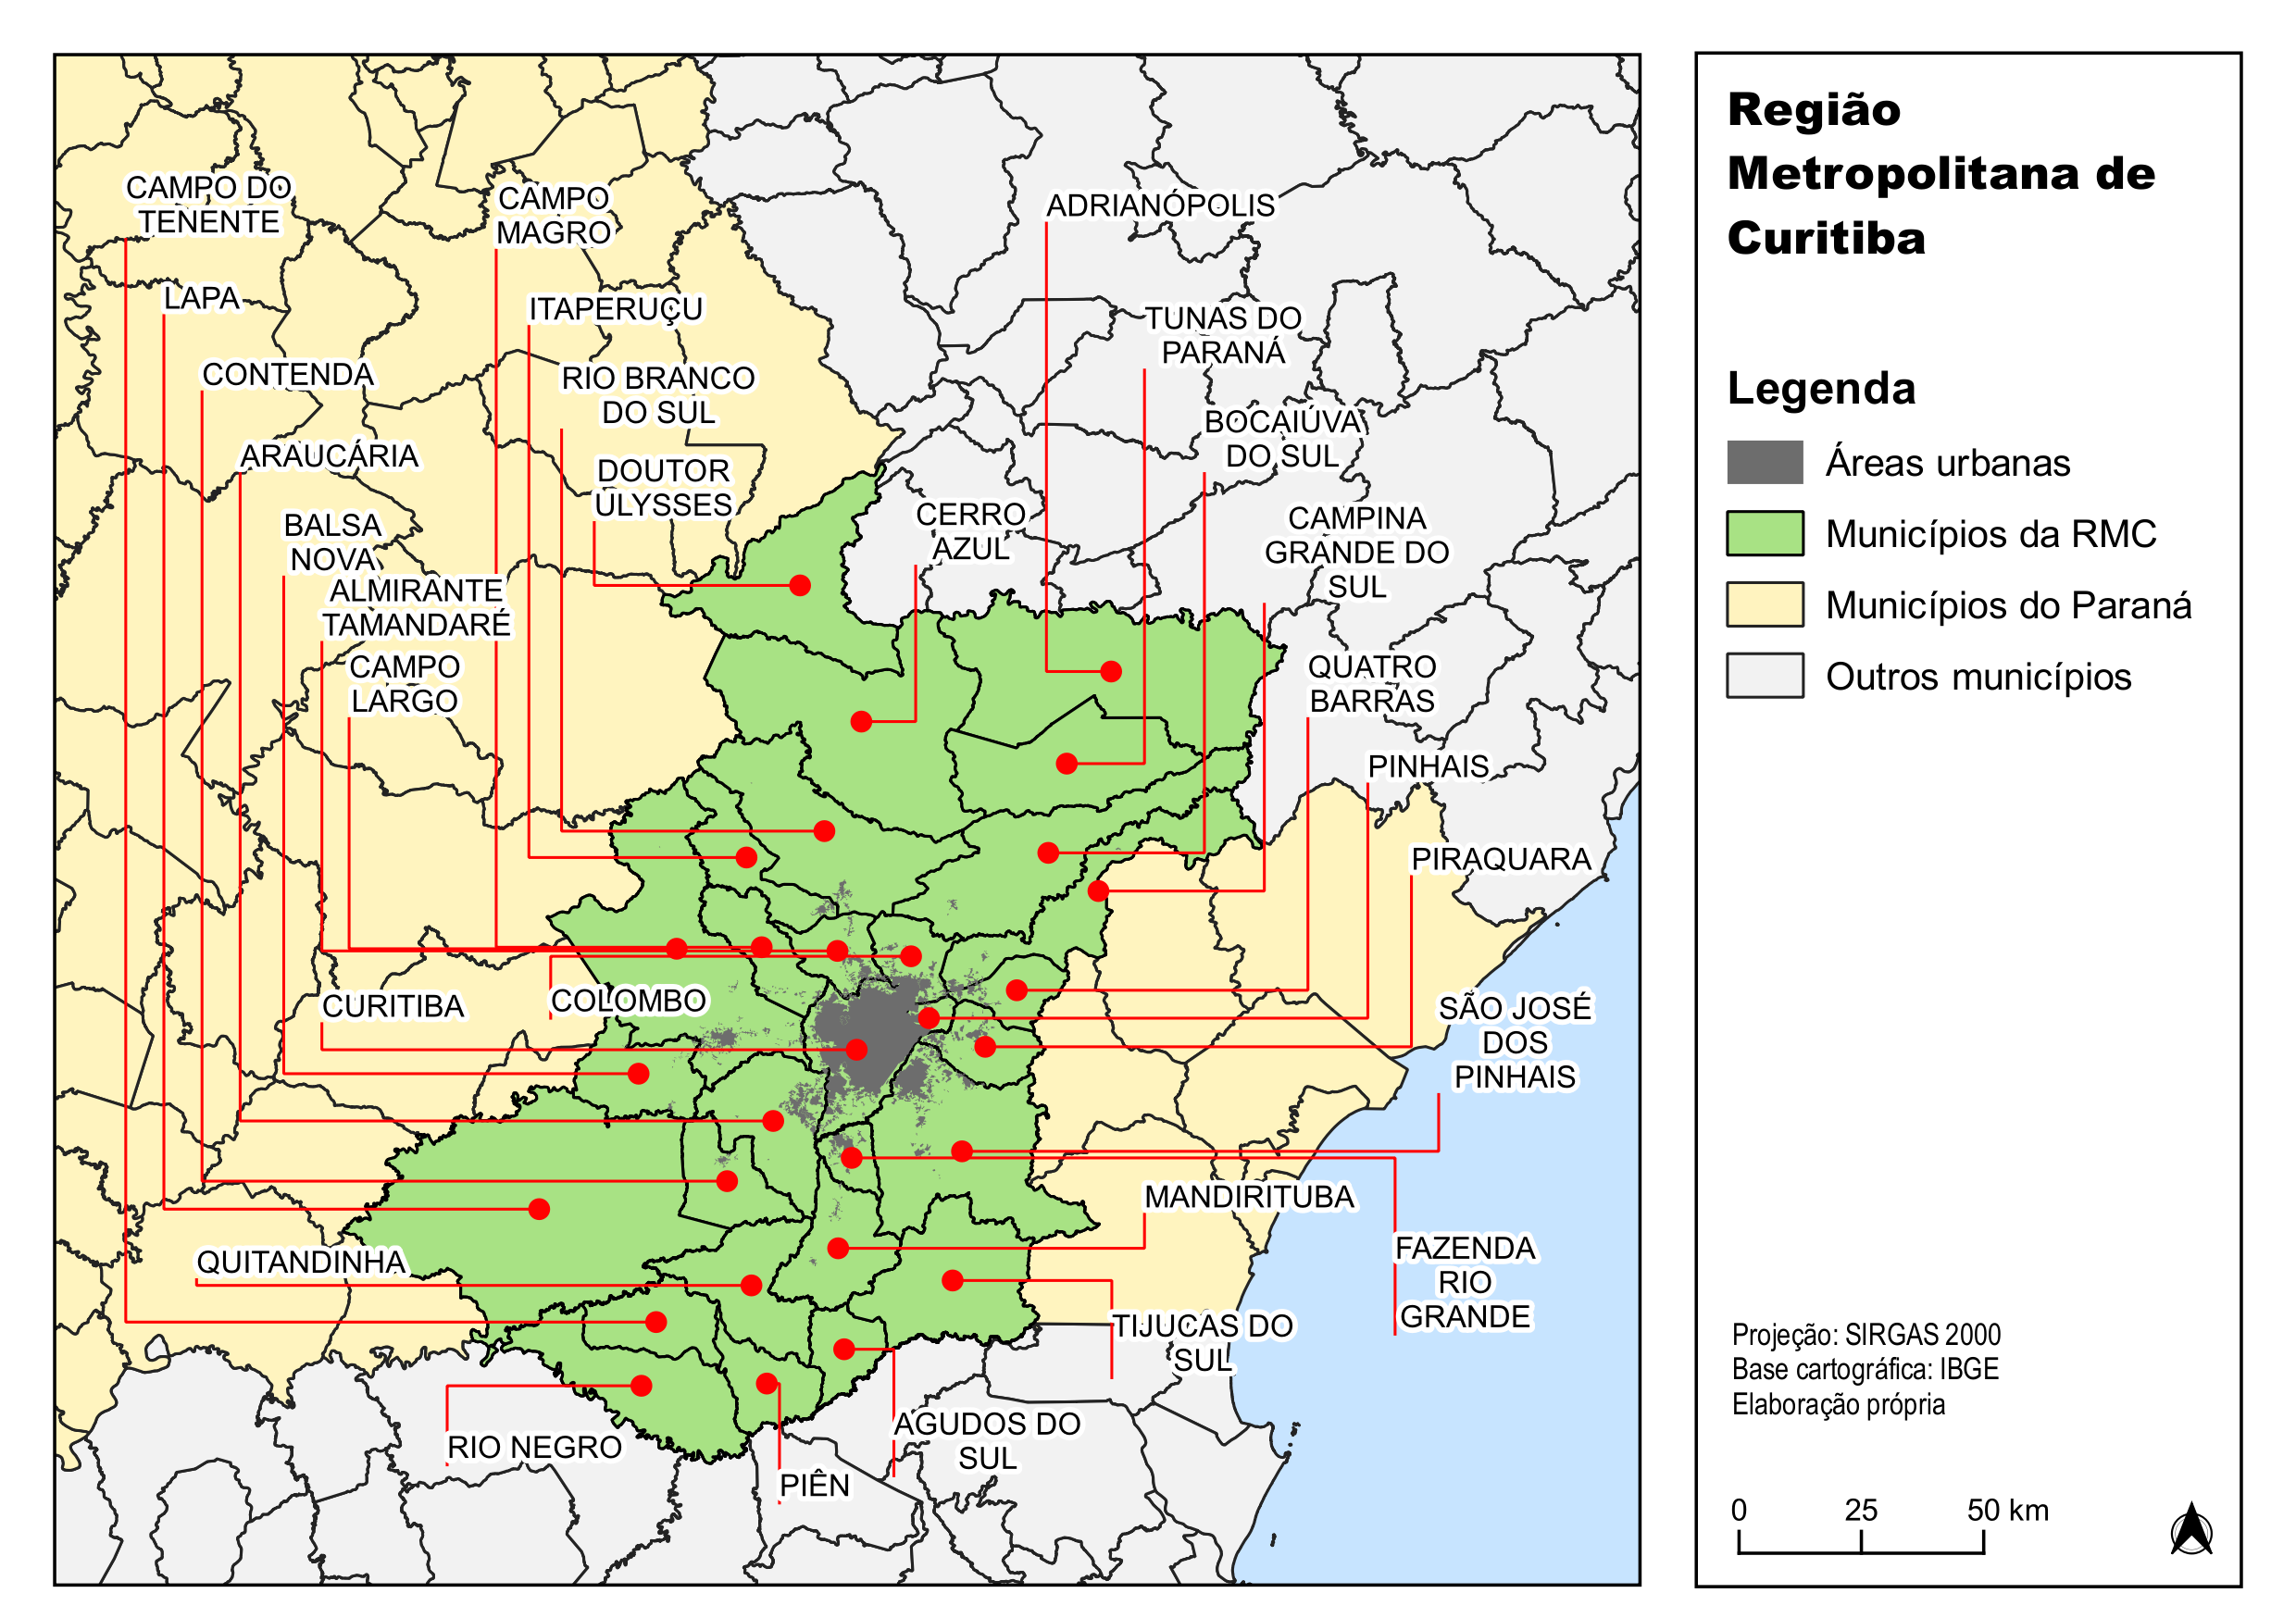
\includegraphics[width=0.85\linewidth]{../gis/produtos/RMC_config_atual}
			\legend{Elaboração própria}
		\end{figure}
	\end{landscape}

	\subsection{Dinâmica populacional}
	
	% TODO rever isso aqui
	A RM de Curitiba reúne cerca de 27\% da população do Estado,  uma proporção menor que a média das regiões metropolitanas do país (38,61\%) (IBGE, 1991 e 1996), mas revela um  crescimento de 266,27\% em relação ao período inicial da aceleração do processo de urbanização regional, nos anos, (Lima, C., Mendonça, F., 2001, p., 140).
	
	Entre 1970 e 1980, o crescimento da RMC foi resultado de um movimento geral de metropolização do país e da elevada migração. Os censos mostram que a população da RM de Curitiba passou de 869.837 habitantes em 1970 (12,55\% da população do estado do Paraná) para 2.003.015 (23,7\%) em 1991.
	
	A partir da década de 1990, com o processo de construção de uma imagem da cidade por meio do marketing urbano, aliado a atração de investimentos, se deu o incremento populacional, alcançando ao ano 2000, 2.768.394 (28,95\% do estado) e 3.223.836 em 2010, ou 30,86\% do total estadual, dos quais 1.757.907 pertencem ao município-polo (16,78\% do total do estado) (IBGE, 2012a). Entre 2000 e 2010, o incremento populacional da região foi de 16,36\%, ou 453.364 pessoas a mais. Ao excluir Curitiba, as outras 28 cidades da RM apresentaram variação de 19,59\%, ou 288.305 novos habitantes.
	
	Segundo \citeonline[p. 64]{delgado2014a}, Curitiba é um exemplo nítido da organização social do trabalho e concentração do capital paranaenses, exacerbando um modelo de produção extremamente concentrador, sendo a configuração reforçada por políticas de desenvolvimento estaduais e também outras políticas de organização do espaço urbano, outrossim, para \citeonline[p. 4]{firkowski2002a} ``ao contrário do que se observa ao nível nacional com a desaceleração da concentração populacional nas regiões metropolitanas, no Paraná ocorre exatamente o oposto, ou seja, a exacerbação do movimento concentrador, principalmente na Região Metropolitana de Curitiba''.
	
	\begin{table}
		\centering
		\caption{Brasil, região Sul, Paraná, RM de Curitiba e municípios: estatísticas populacionais (2000-2010)}
		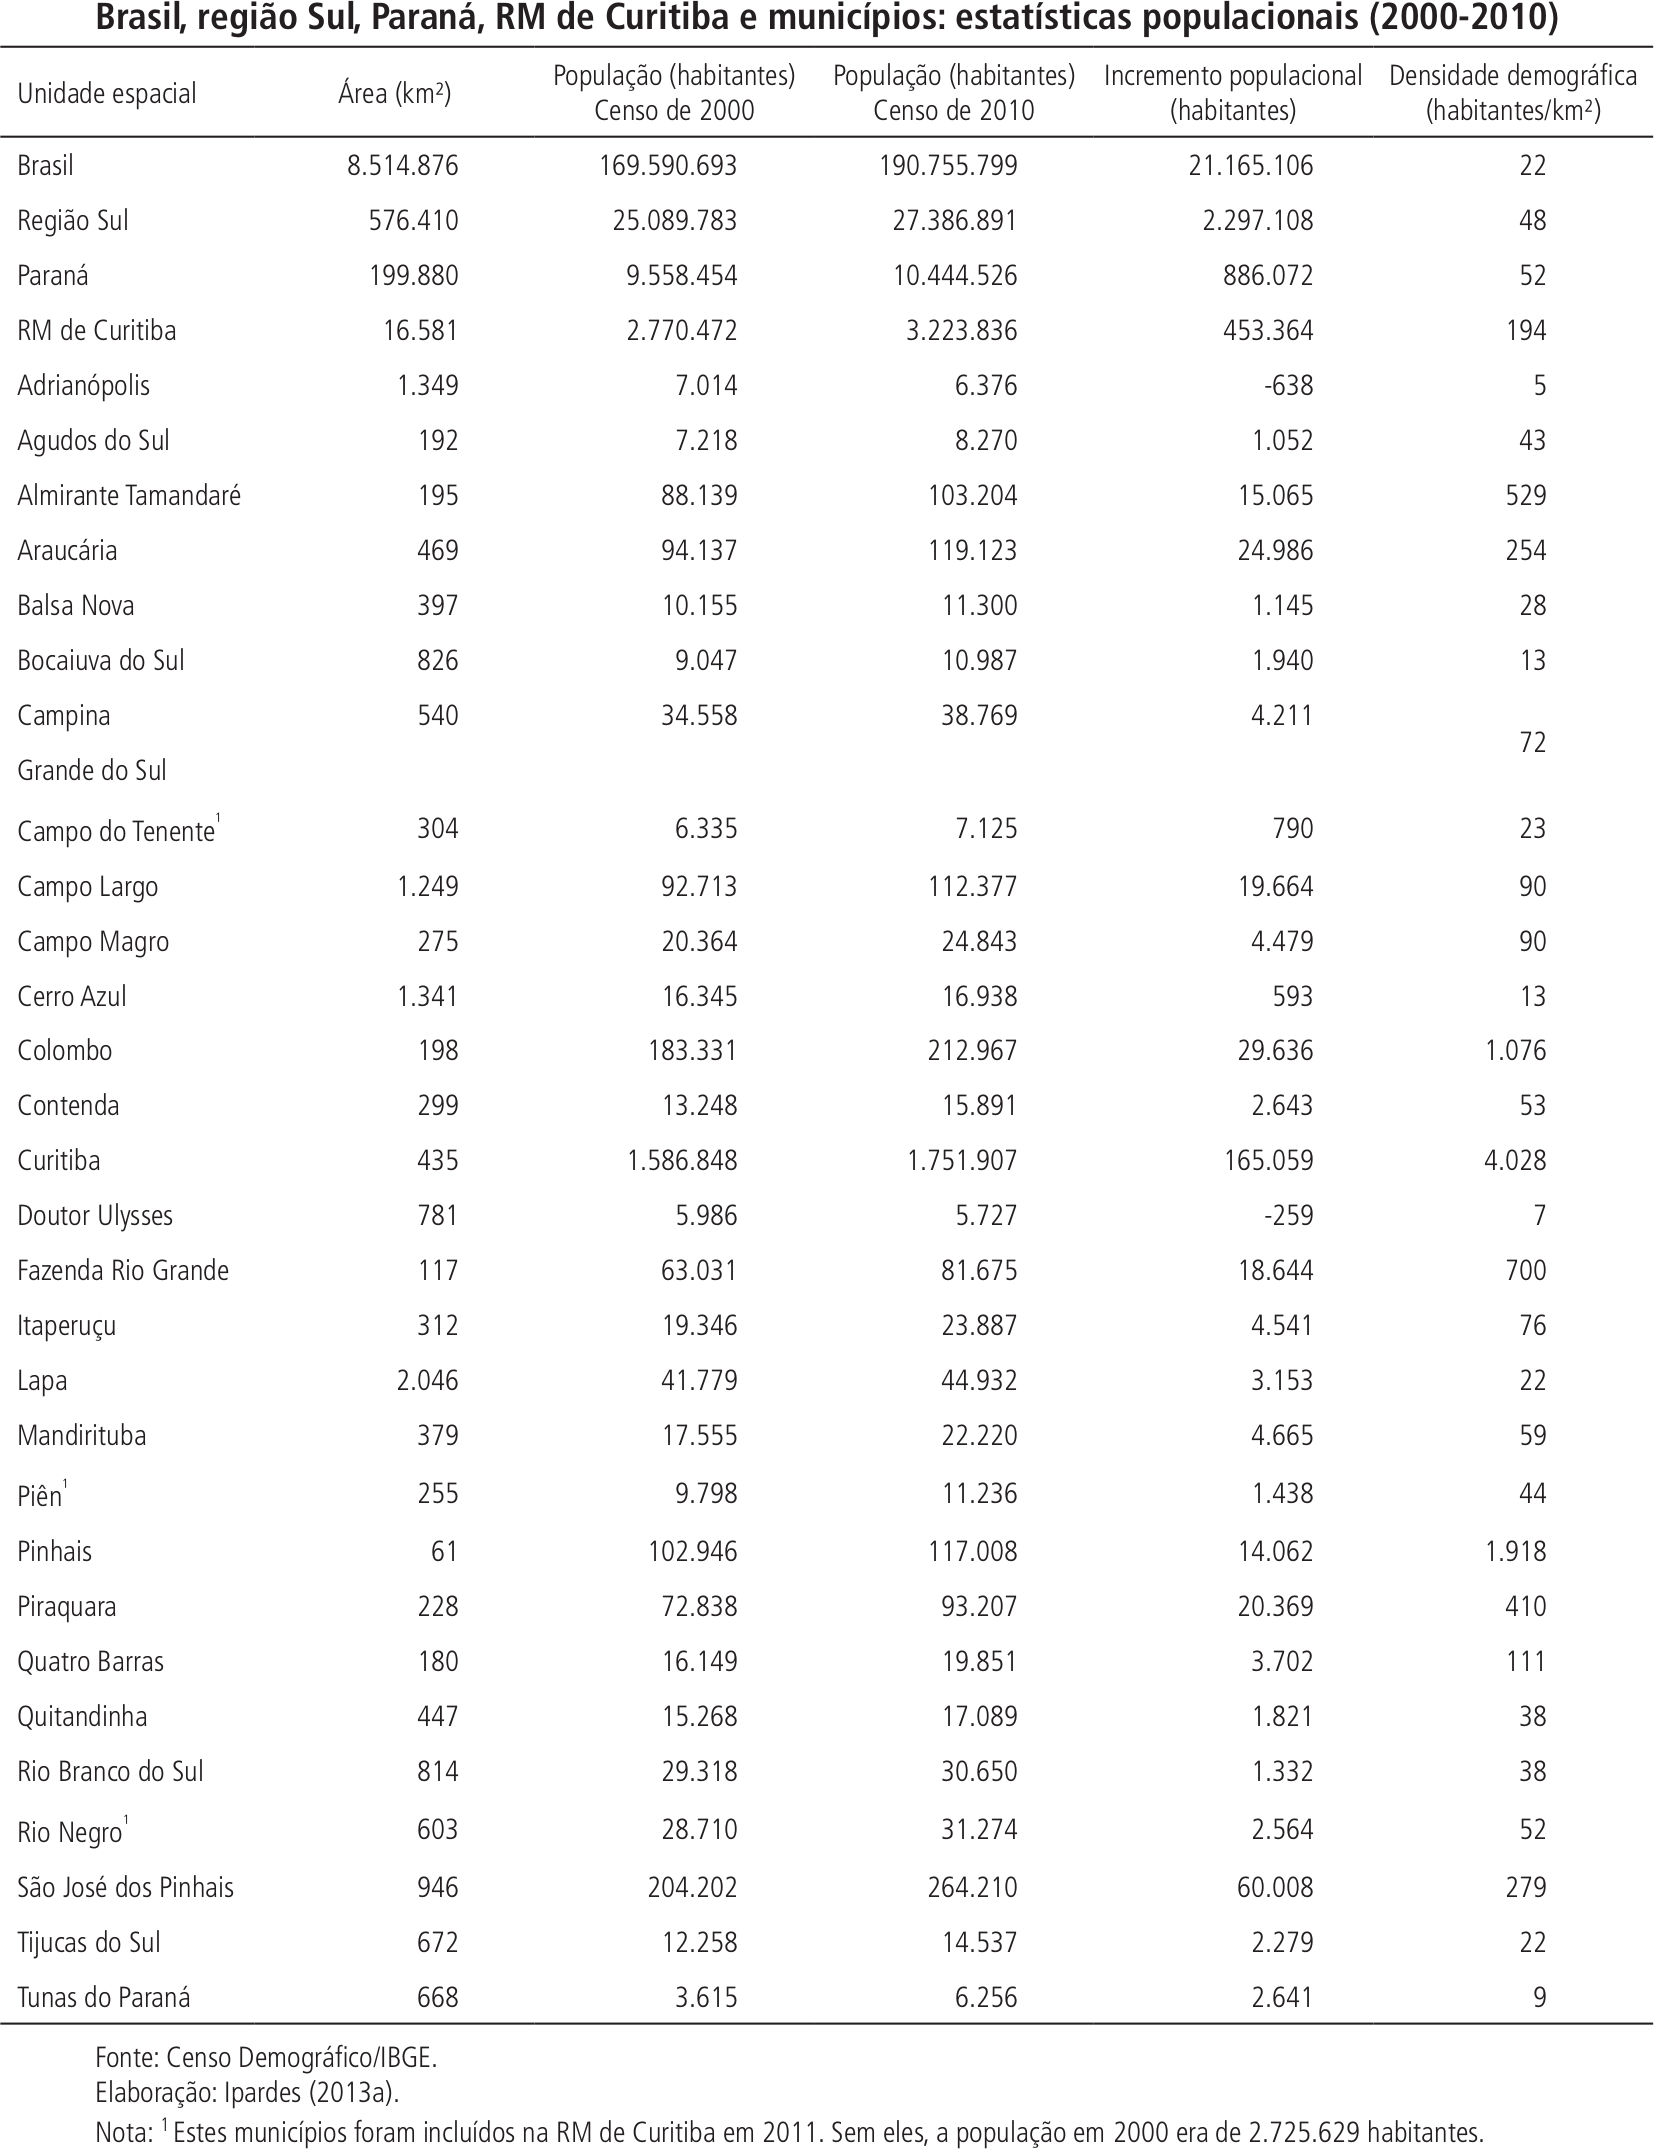
\includegraphics[width=1.0\linewidth]{img/costa2015a_01}
		\label{tab:costa2015a_01}
		\legend{Fonte: \citeonline[p. 9]{costa2015a}}
	\end{table}
	
	Na \autoref{tab:costa2015a_01}, temos as estatísticas populacionais das cidades que compõem a Região Metropolitana de Curitiba, em relação ao Paraná, Região Sul e Brasil no período de 2000 a 2010. É possível observar um incremento populacional significativo em alguns municípios, como Almirante Tamandaré, Araucária, Campo Largo, Colombo, Pinhais, Piraquara, São José dos Pinhais e Curitiba, ao passo que municípios como Adrianópolis e Doutor Ulysses estão perdendo população. 
	
	De acordo com as estatísticas apresentadas na \autoref{fig:costa2015a_02}, em termos gerais (agregados) juntas, a população das cidades da Região Metropolitana tendem a ser equivalentes a de Curitiba, ou até mesmo ultrapassá-la antes da década de 2030.
	
	\begin{figure}
		\centering
		\caption{RM de Curitiba e RM de Curitiba sem Curitiba: projeção populacional (1980-2023)}
		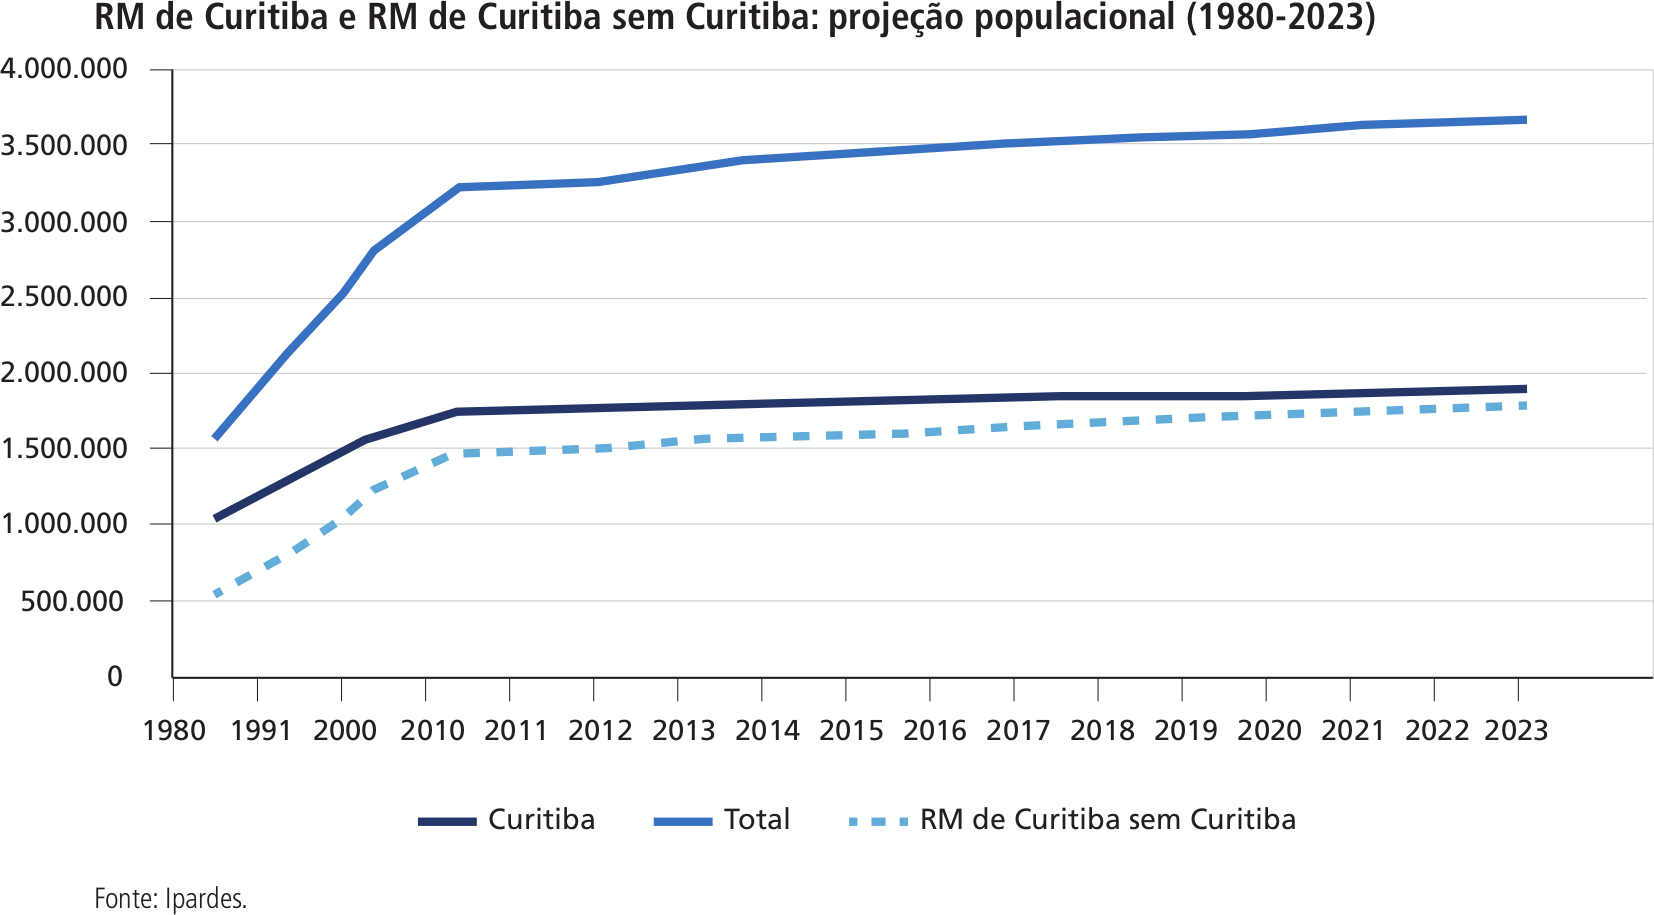
\includegraphics[width=1.0\linewidth]{img/costa2015a_02}
		\label{fig:costa2015a_02}
		\legend{Fonte: \citeonline[p. 10]{costa2015a}}
	\end{figure}
	
	Destes municípios, há um diferente grau de integração, uma vez que alguns pertencem de fato à aglomeração metropolitana, isto é, o \gls{nuc} e outros que foram inseridos à RM posteriormente, por legislação estadual ou desmembramento, sendo que, o crescimento populacional se dá mais expressivamente nos municípios pertencentes ao \gls{nuc}. Desta forma, o crescimento populacional visto de forma agregada mascara que os municípios das franjas metropolitanas não possuem crescimento expressivo, sendo que alguns deles inclusive apresentam redução populacional.
	
	A partir das considerações de \citeonline[p. 10]{costa2015a}, vale ressaltar que, em muitos casos, há uma fragmentação da mancha urbana. Segundo o \citeonline{ipardes2006a}, o fenômeno de espraiamento da população sobre os municípios pertencentes ao que é classificado hoje como o \gls{nuc} se iniciou na década de 1970, cujo espaço de consolidação foi se dando em áreas ao norte dos municípios e as áreas adjacentes ao polo, fazendo com que surgissem vazios entre tais áreas e as suas respectivas sedes municipais. Como exemplo, são apontados os municípios de Almirante Tamandaré, Araucária, Campo Largo e Colombo, em que a distância que possuem de suas sedes municipais são expressivas dessas circunstâncias.
	
	\begin{figure}
		\centering
		\caption{Mapa do \gls{nuc} (2012)}
		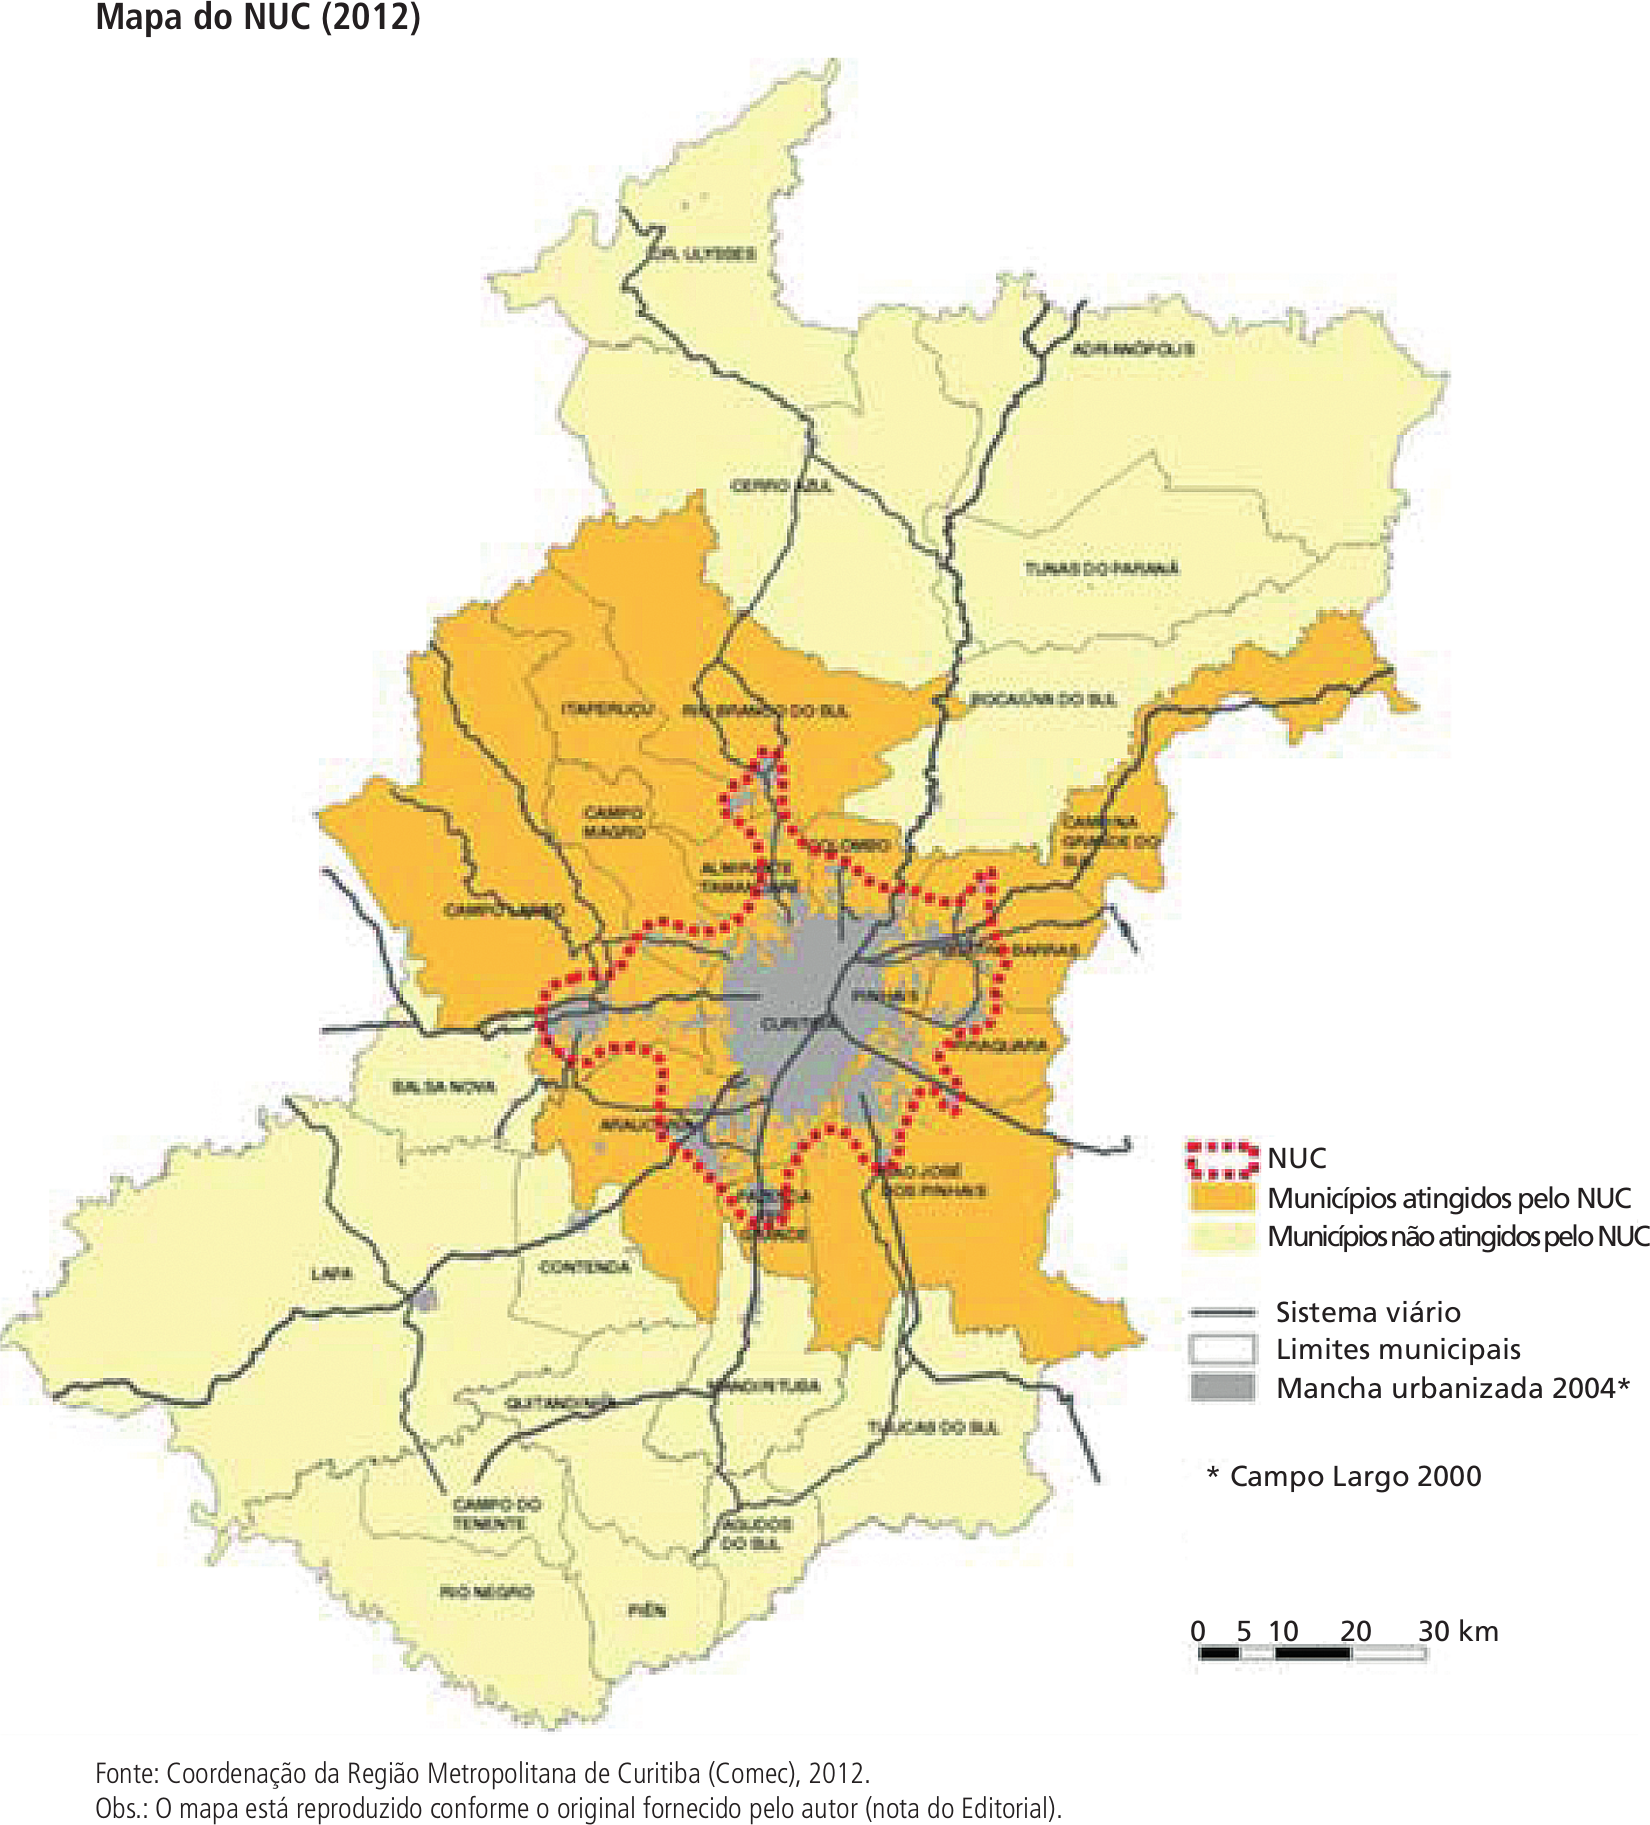
\includegraphics[width=1.0\linewidth]{img/costa2015a_03}
		\label{fig:costa2015a_03}
		\legend{Fonte: \citeonline[p. 11]{costa2015a}}
	\end{figure}
    
	Em relação ao município de Curitiba, seu crescimento foi direcionado, nos últimos anos para as regiões ao sul, além das áreas limítrofes com outros municípios. O Censo de 2010 mostram esse fato por meio do mapa de incremento populacional nos bairros curitibanos nos anos 2000 a 2010 \cite[p. 11]{costa2015a}.
    
	\begin{figure}
		\centering
		\caption{Bairros com maior incremento absoluto populacional (2000-2010)}
		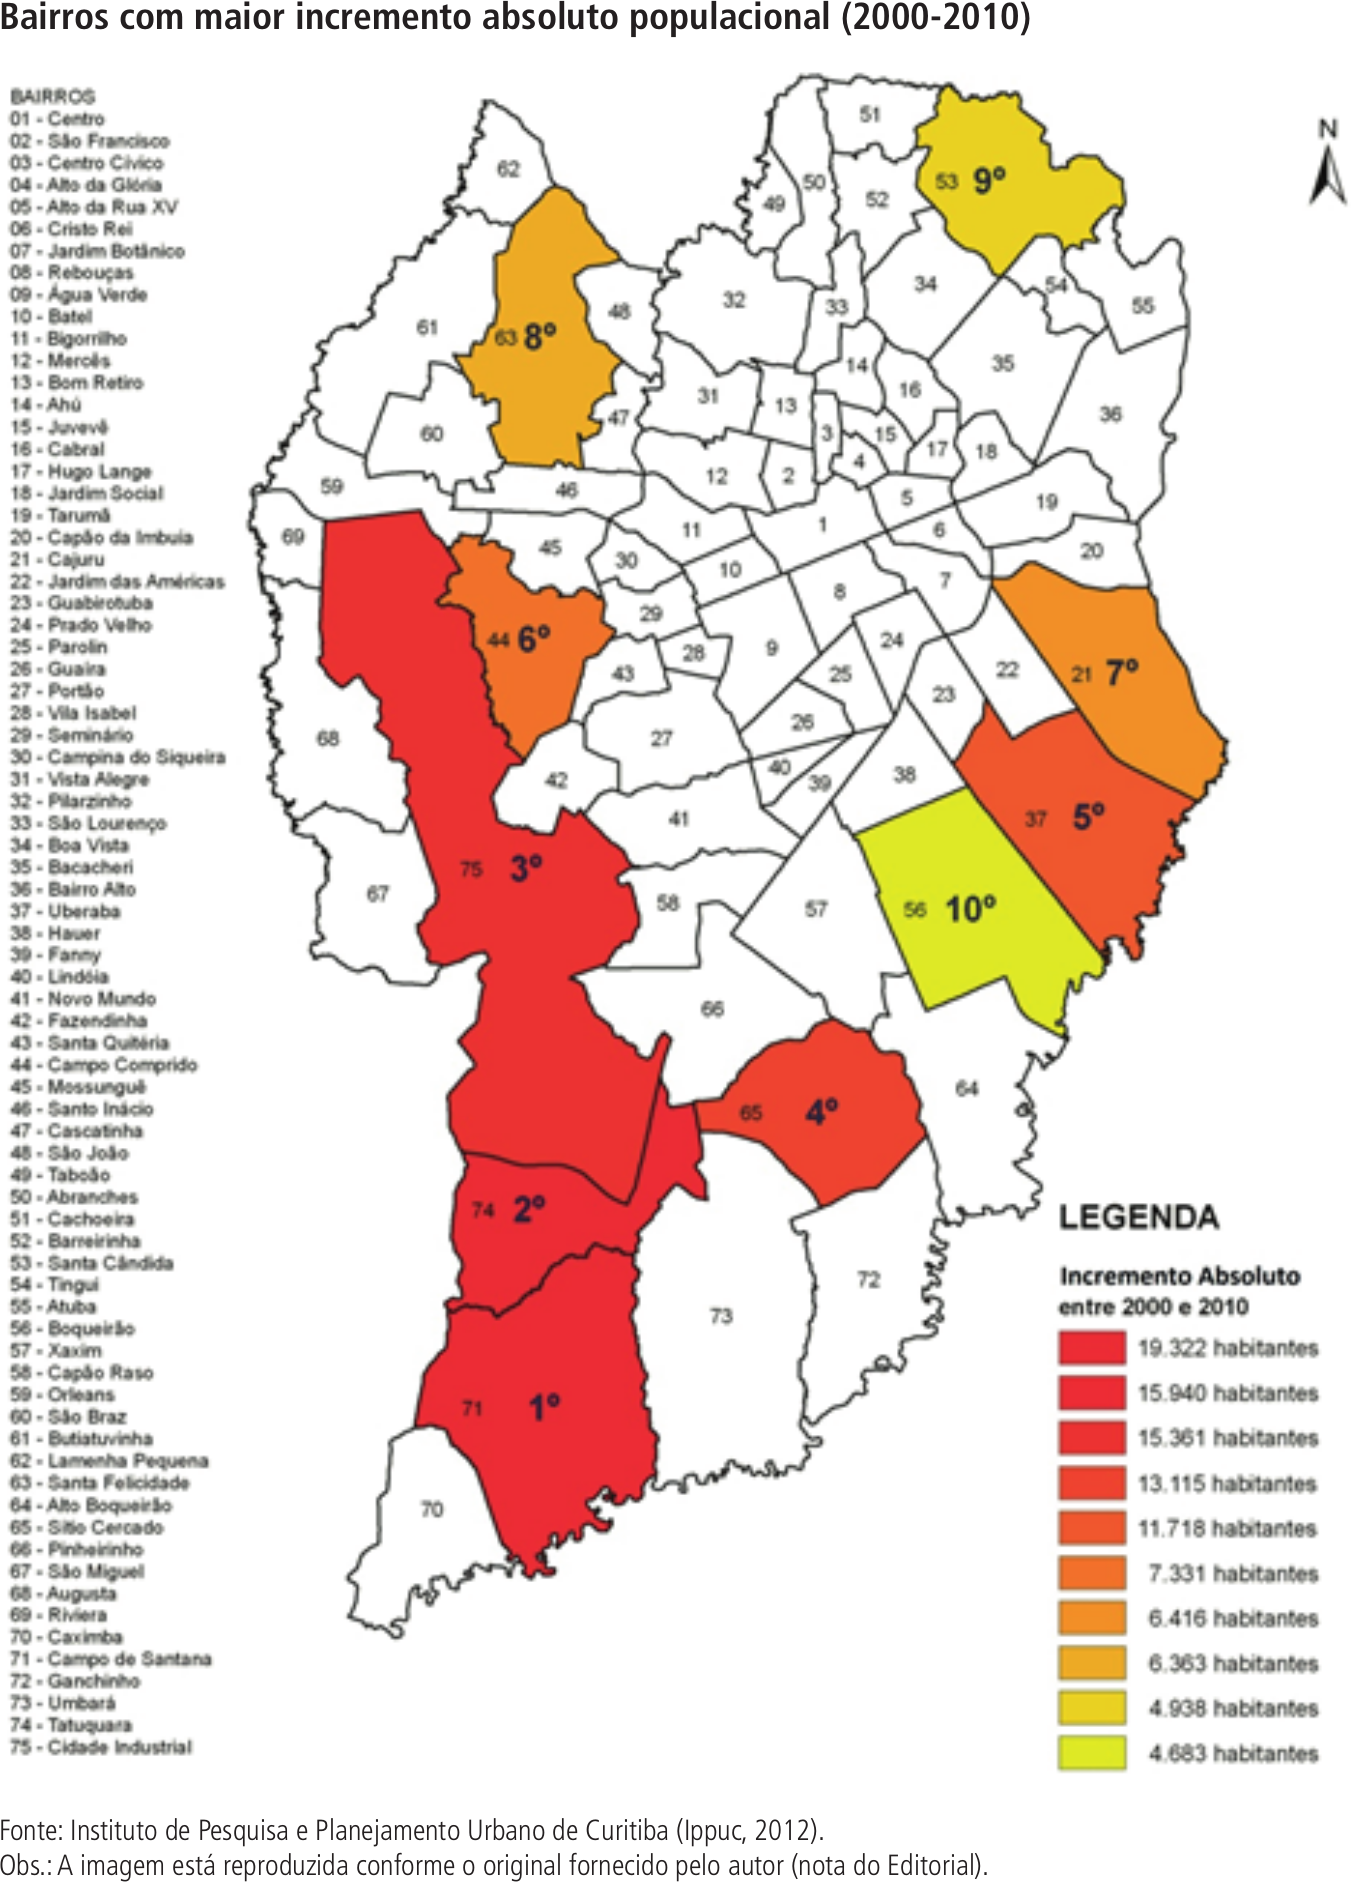
\includegraphics[width=1.0\linewidth]{img/costa2015a_04}
		\label{fig:costa2015a_04}
		\legend{Fonte: \citeonline[p. 12]{costa2015a}}
	\end{figure}
    
	\subsection{Meio físico}
		
	% TODO - mais copia e cola: p. 30 do relatório do IPEA
	Segundo consta em estudos do IPEA, a legislação que versa sobre os recursos hídricos e proteção ambiental tem largo alcance na gestão da RM de Curitiba. Além da legislação federal, a legislação estadual possui uma série de documentos que fazem referência a esta função, como o Decreto Estadual no 6.194/2012 que declara as áreas de interesse de mananciais de abastecimento público. Contudo, a principal lei ligada aos recursos hídricos e proteção ambiental é a Lei Estadual no 12.248/1998. A Lei número 12.248/1998, conhecida como ``Lei dos Mananciais'', adota novos conceitos de gestão do uso e ocupação do solo dos mananciais da RM de Curitiba e concebe, a partir de necessidades identificadas, o ``tratamento diferenciado de áreas de manancial sob pressão por ocupação, compartilhamento do processo de decisão, entre estado e municípios, e a necessidade de um efetivo monitoramento e fiscalização do uso e ocupação do solo'' (Comec, 2013a). Entre outras inovações, esta Lei levou à criação do Sigprom, focado em variáveis de uso e ocupação do solo, buscando garantir, recuperar e preservar as características e condições necessárias para a manutenção dos mananciais para abastecimento. Os mecanismos de ação do Sigprom na gestão do uso e ocupação são, entre outros, as UTPs e APAs (que aglutinam áreas de diferentes municípios que devem ser trabalhadas em conjunto), o CGM (seu órgão máximo), que serão detalhados a seguir, além do Plano de Proteção Ambiental e Reordenamento Territorial (Ppart) em Áreas de Proteção aos Mananciais e do FPA, detalhado na seção 5. Entre os principais instrumentos de gestão, as UTPs são áreas de uso restritivo, ambientalmente frágeis, especialmente as do leste metropolitano, onde estão os mananciais e que estavam sendo sistematicamente ocupadas irregularmente há quase uma década. Os recortes territoriais das UTPs recebem zoneamento especial, de forma a reordenar o uso e ocupação do solo. Foram implantadas cinco UTPs na região.
	
	\begin{landscape}
		\begin{figure}
			\centering
			\caption{Unidades de conservação e hidrografia da \glsdesc{rmc}}
			\label{fig:rmcconservacao}
			\includegraphics[width=0.85\linewidth]{../gis/produtos/RMC_unid_conservacao}
			\legend{Elaboração própria}
		\end{figure}
	\end{landscape}
	
	\subsection{Mobilidade pendular}
	% feito por Caio ou Michele
	
	Conforme \citeonline[p. 12]{costa2015a}, os dois principais motivos de deslocamento entre os municípios da RM são estudo e trabalho, sendo que este último ocupa a primeira posição. De acordo com os dados do Censo das 2,4 milhões que estudavam ou trabalhavam, 384.754 delas se deslocavam por esses motivos, isto é, cerca de 16\%).
	
	Na mesma linha, 318.298 pessoas trabalhavam em um município distinto do local de moradia, dentre os 1.657.198 trabalhadores que vivem na Região Metropolitana de Curitiba, isto equivale a aproximadamente 19\%. Ao olhar exclusivamente para Curitiba, esse número é de 6,3\% \apud{cintra2012a}{costa2015a}.
	
	Tal processo ocorre com mais relevância entre os municípios do \gls{nuc}, por mais que haja um grau de integração entre os demais, contudo, ainda se mostra pouco expressivo, conforme destacado nos mapas para fluxos de trabalho (\autoref{fig:costa2015a_05} e \autoref{fig:costa2015a_06}) e estudo (\autoref{fig:costa2015a_07} e \autoref{fig:costa2015a_08}).
	
	\begin{figure}
		\centering
		\caption{RM de Curitiba: fluxo de entrada para trabalho (2010)}
		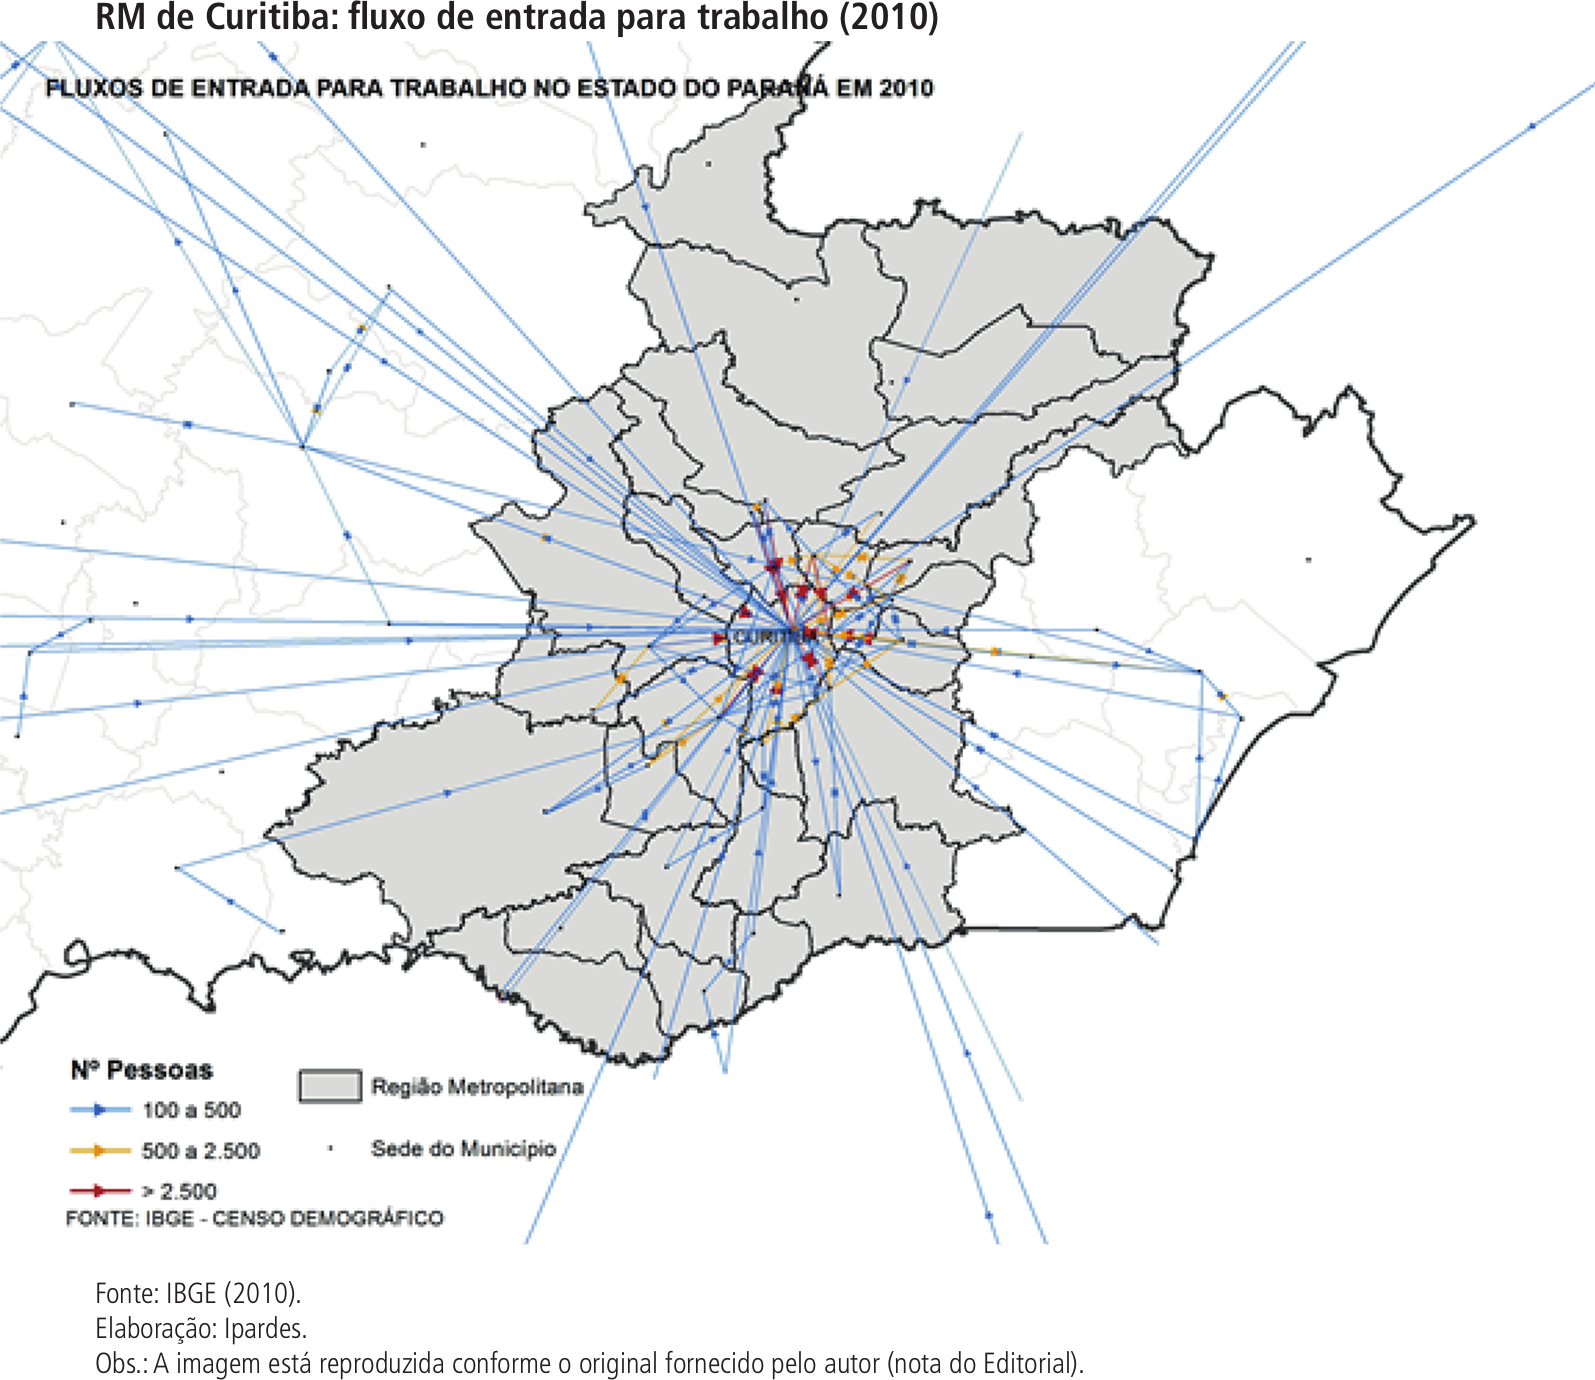
\includegraphics[width=1.0\linewidth]{img/costa2015a_05}
		\label{fig:costa2015a_05}
		\legend{Fonte: \citeonline[p. 14]{costa2015a}}
	\end{figure}

	\begin{figure}
		\centering
		\caption{RM de Curitiba: fluxo de saída para trabalho (2010)}
		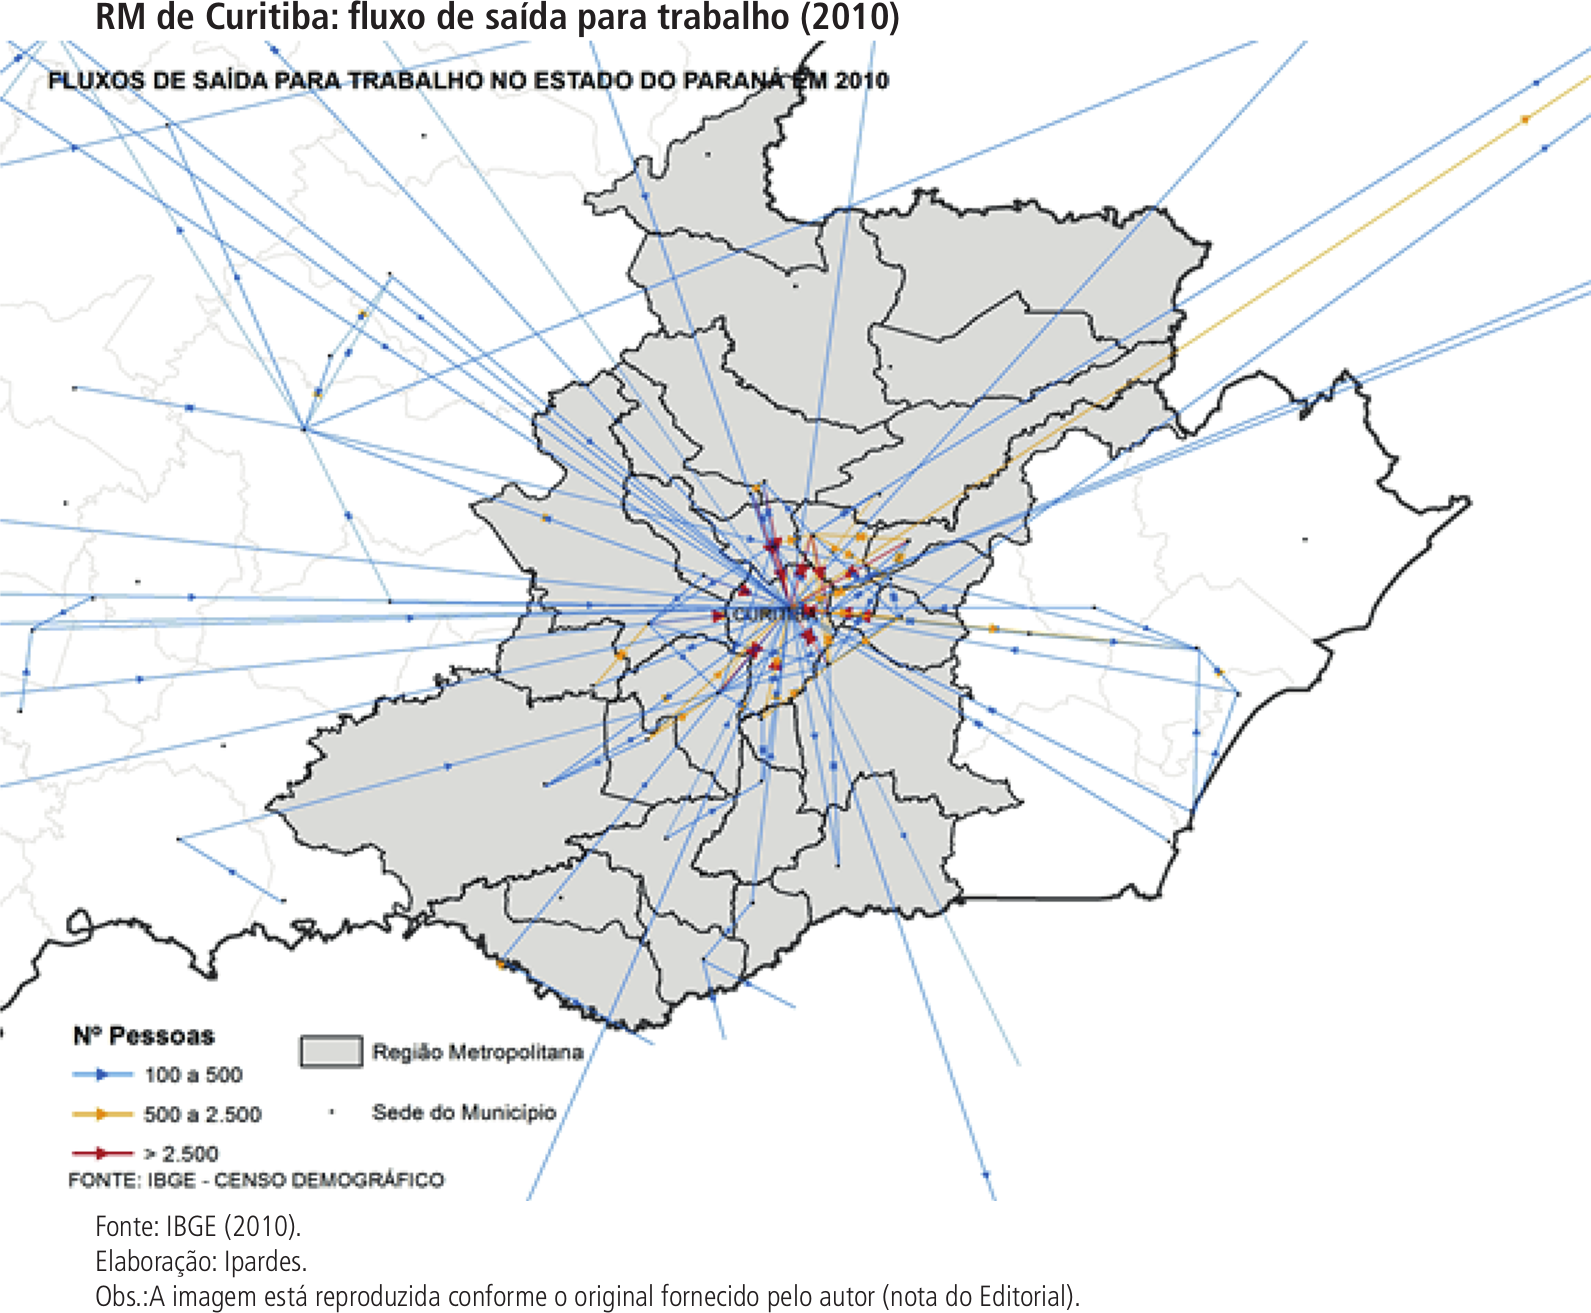
\includegraphics[width=1.0\linewidth]{img/costa2015a_06}
		\label{fig:costa2015a_06}
		\legend{Fonte: \citeonline[p. 14]{costa2015a}}
	\end{figure}
	
	\begin{figure}
		\centering
		\caption{RM de Curitiba: fluxo de entrada para estudo (2010)}
		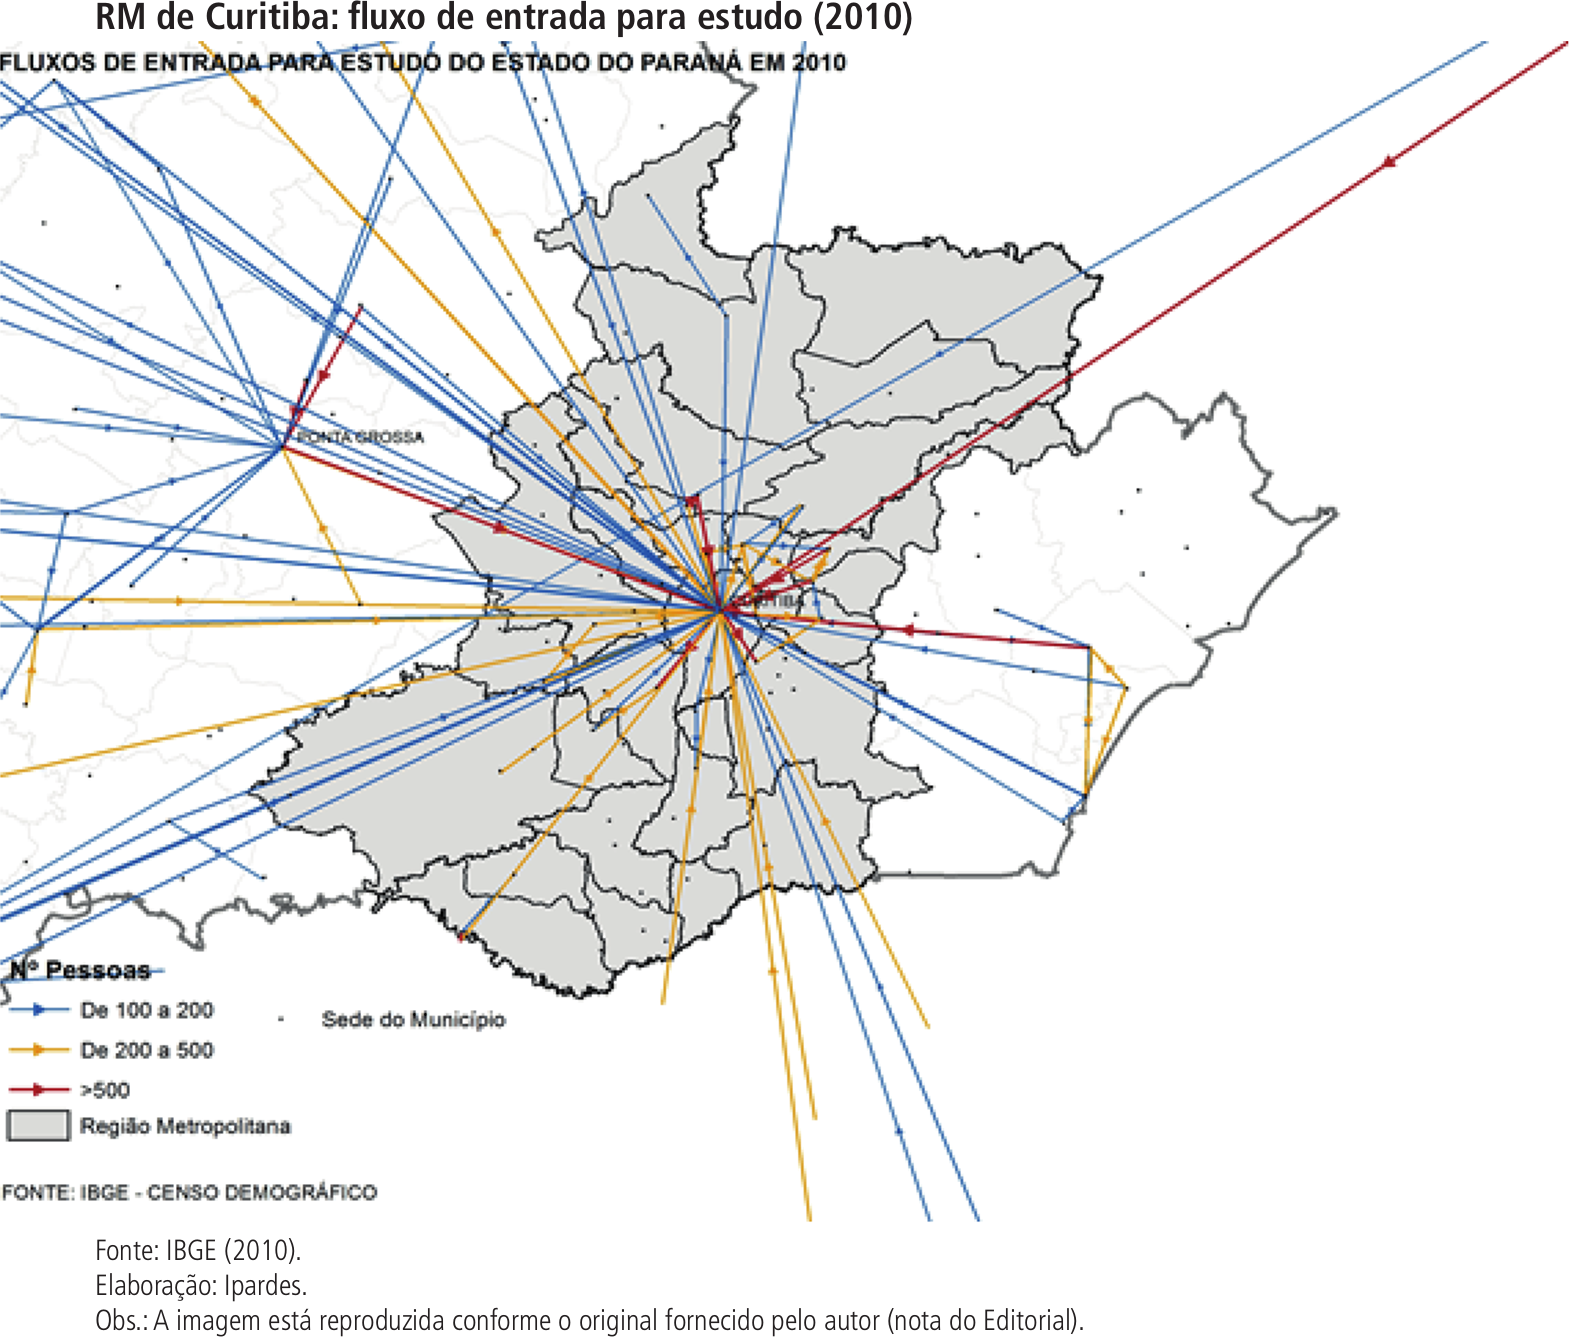
\includegraphics[width=1.0\linewidth]{img/costa2015a_07}
		\label{fig:costa2015a_07}
		\legend{Fonte: \citeonline[p. 15]{costa2015a}}
	\end{figure}

	\begin{figure}
		\centering
		\caption{RM de Curitiba: fluxo de saída para estudo (2010)}
		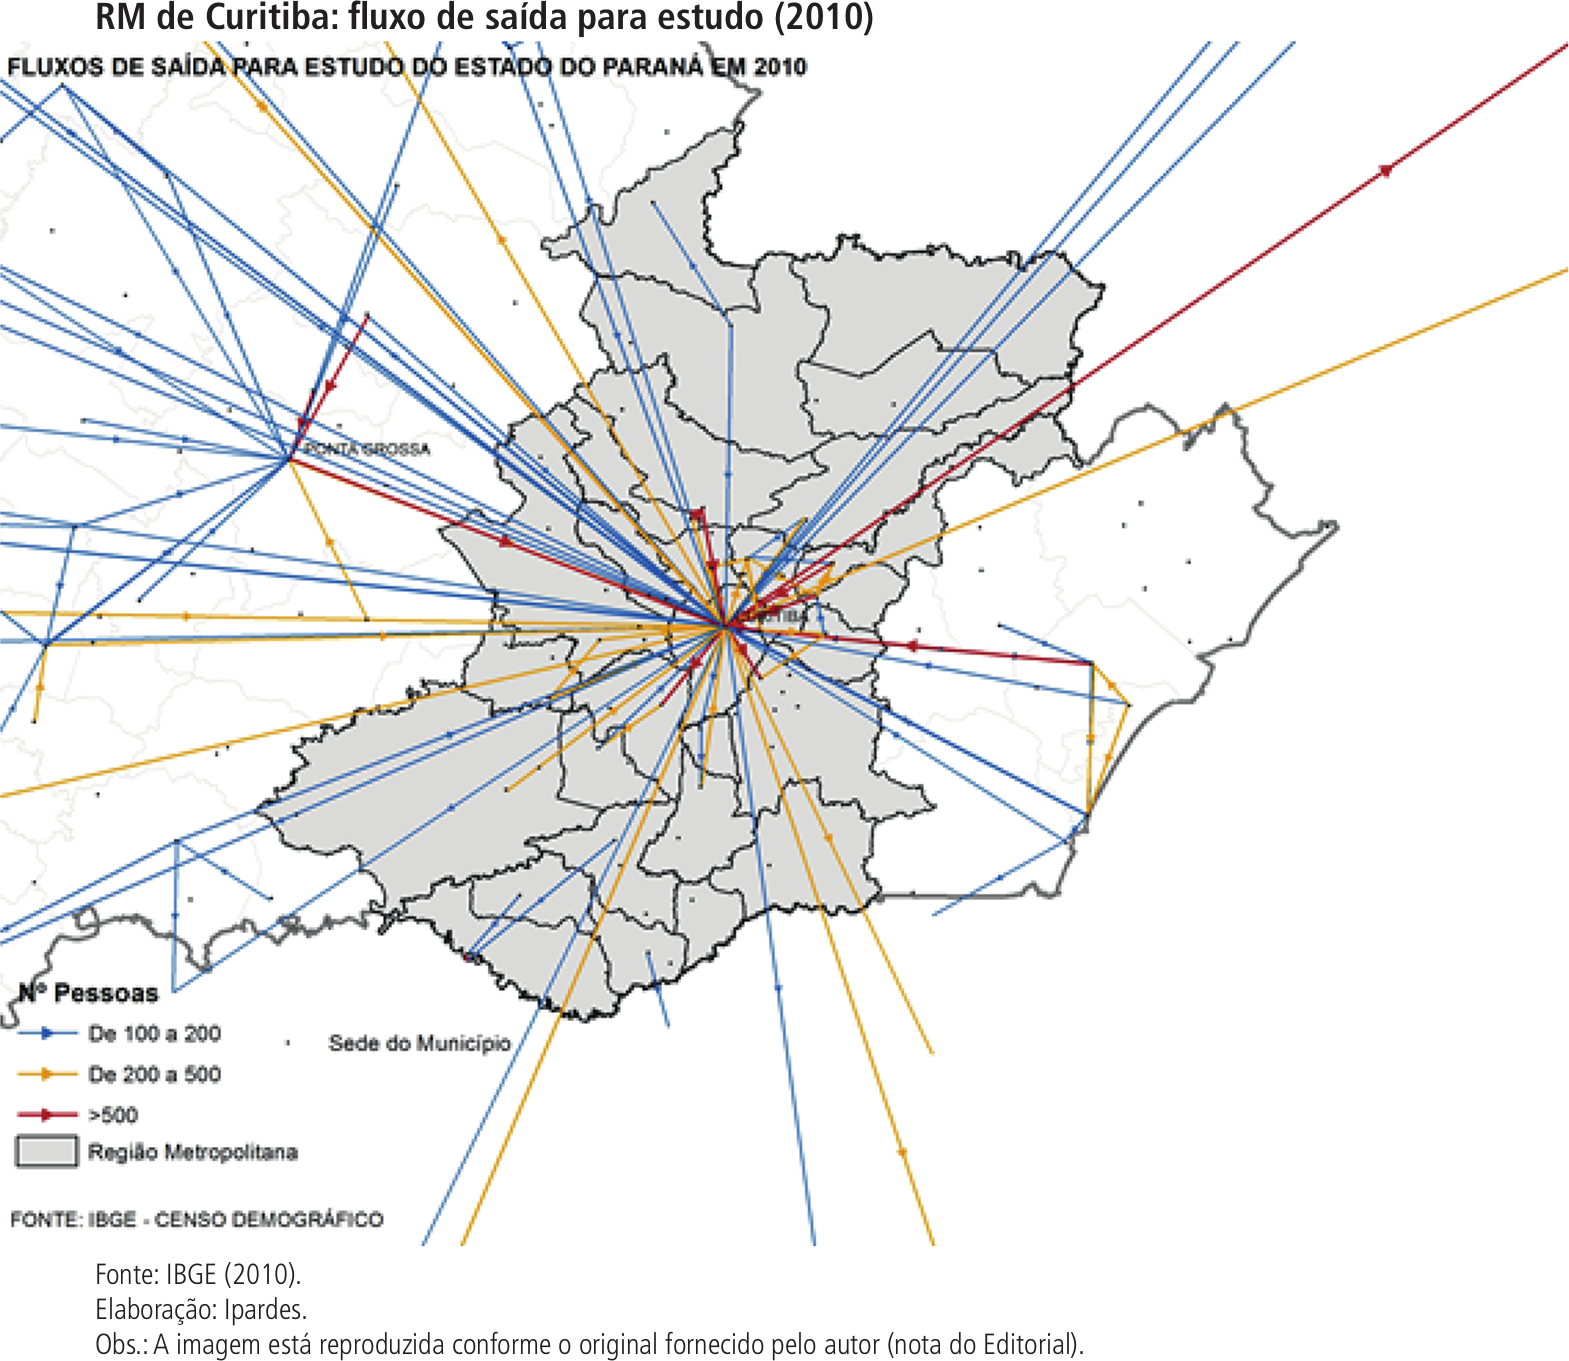
\includegraphics[width=1.0\linewidth]{img/costa2015a_08}
		\label{fig:costa2015a_08}
		\legend{Fonte: \citeonline[p. 15]{costa2015a}}
	\end{figure}
	
	\subsection{Aspectos econômicos e processo econômico-produtivo}
	% reescrito por Michele, recebeu mais algumas coisas por parte do Caio
	
	As décadas de 70 e 80 foram marcadas por uma concentração industrial no município de Curitiba (\glsdesc{cic} - \gls{cic}), e uma área adjacente que atingia o município de Araucária, em seu centro industrial (\gls{ciar}). No entanto, seu padrão se dava de forma fragmentada no interior de ambos. Já na década de 90, a indústria se mostra desconcentrada no espaço urbano ampliado e mais concentrada no interior de alguns distritos. Apesar do processo de desconcentração, iniciado nos anos 70, a \gls{rmc} segue sendo o destino das principais capitais industriais, como também das pessoas \cite{firkowski2002b}.
	
	\citeonline[p. 61]{lourenco2009a} também menciona a implantação de um polo cimenteiro na \glsdesc{rmc} na primeira metade dos anos 1970, mesma época na qual a modernização agrícola (introdução da soja e do trigo) e agroindustrial se deu.
	
	Um exemplo do desenvolvimento industrial em Araucária é citado por \citeonline[p. 54]{castro2005a}:
	
	\begin{citacao}
		``Curitiba também cresce no sentido oeste, ao criar uma área destinada às atividades industriais. A instalação da Refinaria Petrobrás em Araucária também promoveu o desenvolvimento da região oeste de Curitiba, transpondo as fronteiras entre os municípios de Curitiba e Araucária.''
	\end{citacao}
	
	\citeonline[p. 62]{lourenco2009a} avalia o surgimento dos dois núcleos industriais como parte de uma trajetória de desconcentração industrial observada na segunda metade da década de 1970, apontando uma série de atores que atuaram durante o governo do ditador Ernesto Geisel:
	
	\begin{citacao}
		``O terceiro estágio de mudanças expressivas verificou-se no segundo quinquênio dos anos 70, com a implantação da \glsdesc{cic} (\gls{cic}) e da Refinaria de Petróleo de Araucária. Tais acontecimentos reproduziram parte da trajetória de desconcentração industrial experimentada pelo país entre 1975 e 1979 – durante a implantação do II \glsdesc{pnd} (\gls{pnd}), no governo Geisel ---, decorrente de substanciais pressões políticas regionais junto aos órgãos federais gestores dos incentivos fiscais e financeiros, como o \glsdesc{cdi} (\gls{cdi}), o \glsdesc{befiex}
		(\gls{befiex}) e o \gls{bndes}.'' \cite[p. 62]{lourenco2009a}
	\end{citacao}

	São José dos Pinhais é apontado como um indicador importante de mudanças na localização das indústrias \cite{firkowski2002b}, dado que apresenta uma inversão no modelo de ocupação, uma vez que o vetor de expansão fomentado que sempre foi localizado à oeste, e São José dos Pinhais passa a ser direcionado de forma contrária, a Leste. E é nessa região que predomina a concentração das indústrias, revelando conflitos importantes em relação ao uso do solo e questão ambiental.

	O contexto tratado aqui se refere ao modelo de produção flexível, em que a ocupação no espaço não ocorre sob uma mesma planta, mas em seu entorno. Essa abordagem se desdobra em um território particular, se diferenciando do período anterior, sendo assim, há um maior processo de interdependência, o que não permite que a escolha localizacional de uma grande empresa ocorra de modo aleatório. Nesse padrão, o território ganha importância e passa a ser definidor, é nele que as trocas ocorrem, as relações se estabelecem e a disputa se dá. 
	
	Nos anos finais da década de 1970, a Volvo foi instalada em Curitiba, mas não fomentou a chegada de outras empresas no mesmo padrão que vemos hoje. A ocupação ocorreu com base no uso do solo, sendo o local uma área separada exclusivamente para o uso industrial, mas que na prática não representa uma homogeneidade do setor, pelo contrário, o entorno representa uma variedade.
	
	Hoje, nota-se que a implantação das indústrias automobilísticas se caracterizam por um aspecto mais fechado, com base no modelo de produção flexível, uma vez que a localização é determinada pela montador e os funcionários seguem o padrão. Tais locais, por sua vez, são estipulados de acordo com a ausência de empecilhos, independente de sua natureza, seja ela social ou trabalhista. No caso de Curitiba, as áreas escolhidas foram marcadas pelo novo, aquilo que pode ser feito a partir do início, longe de barreiras. Aliado a isso, há também o aspecto inovador, abarcando tecnologias, infraestrutura, especificamente a rede de fibra óptica, a diversidade de sinergias possíveis, as parcerias, as concentrações imateriais, dentre outros) e atores, levando em consideração que eleger um lugar não está atrelado sobre aos fatores técnicos e econômicos, como também pela conjuntura e as possibilidades a postos.

	Vale destacar que esse modelo reflete em expressivas problemáticas socioespaciais, sobretudo os de caráter ambiental, visto que a localização desses grandes empreendimentos se dá em áreas mais sensíveis e são, muitas vezes, apoiados pelos governos locais e estaduais, pois estes atendem aos desejos dos grupos mais poderosos, a fim de permitir a entrada de capital no local e evitar perder tais oportunidades de ``desenvolvimento''. 
	
	\begin{citacao}
		``[\dots] em todos os níveis da questão ambiental existem interesses conflitantes e, portanto, custos a serem alocados a determinados setores ou determinadas sociedades”, e quando o que está em jogo é a localização de grandes empresas, tais custos tendem a ser socializados pela população da área receptora desses capitais, mesmo que, num primeiro momento, ela não se dê conta de quão alto eles serão no futuro.'' \apudonline[p. 93]{martine1993a}{firkowski2002b}
	\end{citacao}

	\begin{figure}
		\centering
		\caption{Localização industrial com predominância na \gls{rmc} (1970-2001)}
		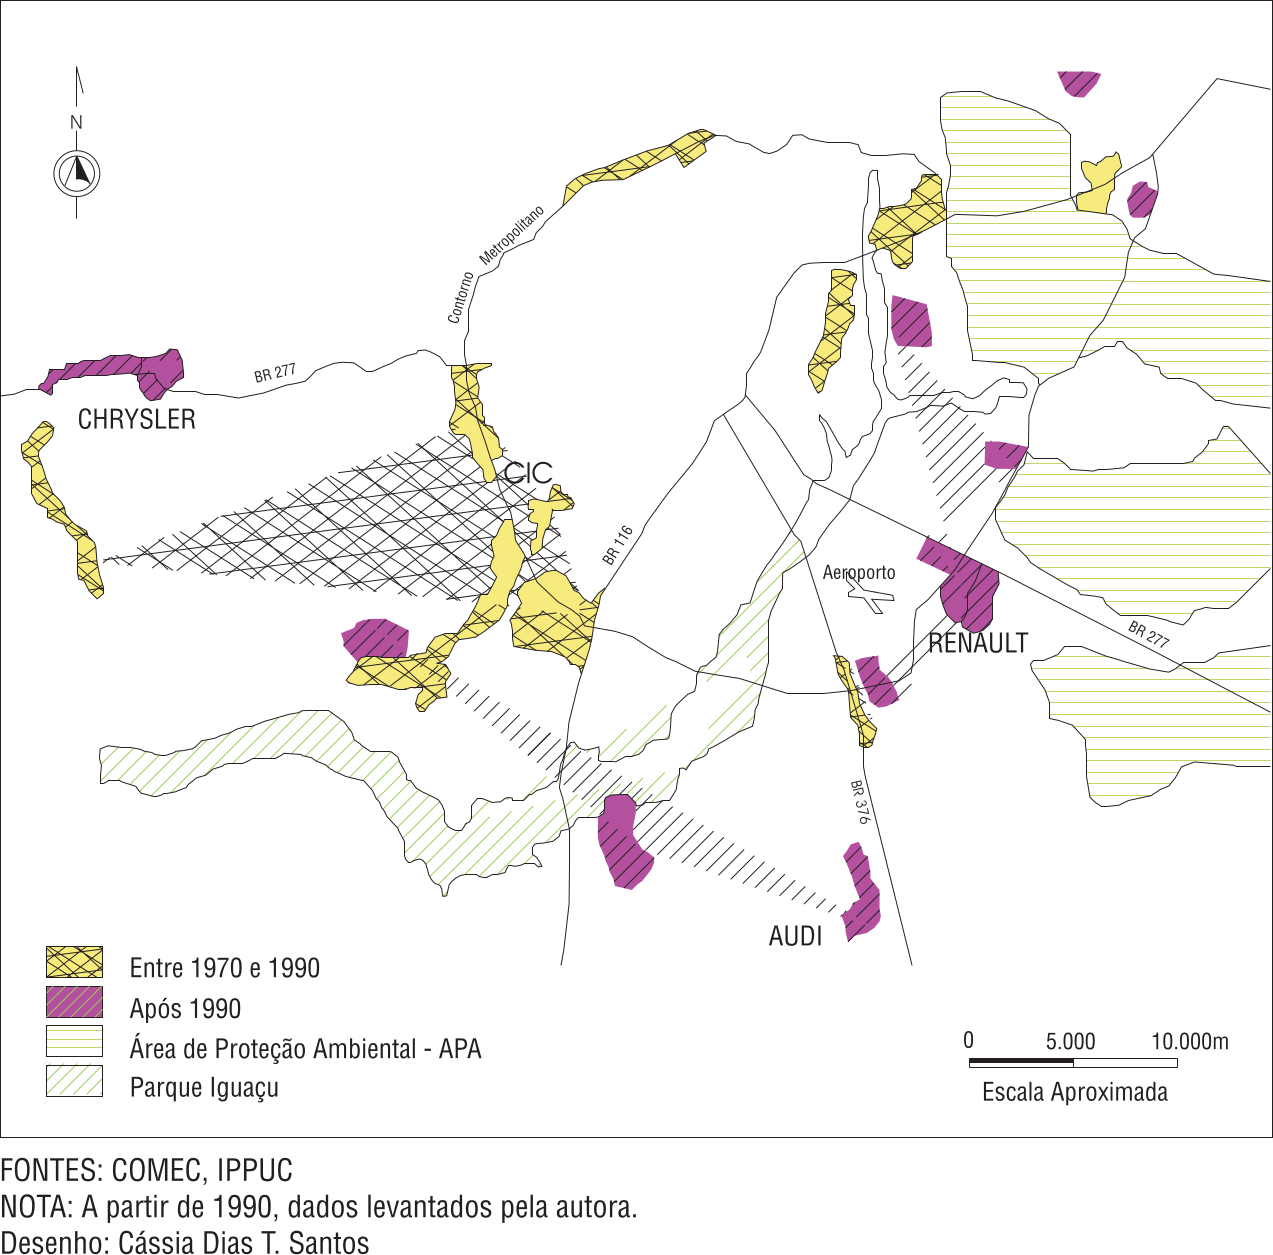
\includegraphics[width=1.0\linewidth]{img/firkowski2002b_01}
		\label{fig:firkowski2002b}
		\legend{Fonte: \citeonline[p. 95]{firkowski2002b}}
	\end{figure}

	O núcleo central da região metropolitana assume papel importante na localização das indústrias, dado que elas estão conectadas a ele, tanto nas últimas décadas quanto em um período mais recente.  Como apontado anteriormente, as questões ambientais são as que mais assinalam os entraves no território. A Renault é um caso clássico, pois sua presença fomentou a vinda de mais indústrias ainda para a região. Além disso, também incentivou o crescimento de outras atividades em seu entorno. 
	
	\begin{citacao}
		``O caso mais notório foi, sem dúvida, o da Renault, que motivou a solução da questão por meio da alteração da área de proteção ambiental, a qual foi fragmentada em três áreas menores, ficando excluídos exatamente os locais onde hoje está implantada a maioria das novas fábricas. Em 18 de março de 1996, o prefeito de São José dos Pinhais assinou a Lei 03/96, de criação do Distrito Industrial de São José dos Pinhais,12 definindo sua localização em área de proteção ambiental, segundo o Decreto Estadual no 2.964/79, às margens do Rio Pequeno. Em 6 de maio de 1996, por meio dos Decretos 1.751/52/53/54, o governo estadual alterou os limites da Área de Proteção Ambiental (APA) existente, dividindo-a em três: APA Estadual do Rio Pequeno, APA Estadual do Iraí e APA Estadual do Piraquara. Portanto, a Lei Municipal que definia o local de implantação da Renault se opôs à legislação estadual por cerca de dois meses, até que esta última foi alterada em benefício do empreendimento.'' \cite[p. 96]{firkowski2002b}
	\end{citacao}

	A partir dos anos 90 as problemáticas se intensificaram ainda mais, visto que as transformações da RM se originaram a partir da ocupação das áreas de mananciais. Nesse contexto, a Lei de Proteção aos Mananciais surgiu como meio de conter o avançando das ocupações irregulares, assegurando por meio das Unidades Territoriais de Planejamento (\gls{utp}) a conservação do meio ambiente com vistas a garantir também o crescimento econômico. Dessa forma, haveria uma maior flexibilidade, permitindo com que houve mais diversificação na ocupação do solo, não estando limitados severamente pela lei. Logo, tais transformações legislativas promoveram outros interesses, que não os ambientais, mas sobretudo os imobiliários, a partir de uma aliança entre o público e o privado.
	
	\subsection{Concentração e Influência da Metrópole}
		
	Segundo \citeonline[p. 10]{costa2015a}, Curitiba é uma cidade polarizadora, que estabelece relações com outras aglomerações, aliado a isso, sua economia garante um papel importante na conformação da rede urbana, fazendo com que sua influência transborde a RM na qual está inserida. Assim sendo, ultrapassa o próximo estado, fazendo conexões até mesmo com alguns municípios de Santa Catarina. Análise esta também reiterada por \citeonline[p. 32]{moura2001a}, que aponta que ``Curitiba tem a peculiaridade de, além de polarizar toda a rede urbana paranaense, transcender sua polarização para o Estado de Santa Catarina, inserindo em sua rede as áreas de abrangência das principais centralidades catarinenses''. A rodovia BR-116 é um eixo articulador importante:
	
	\begin{citacao}
		``A região de influência direta do subsistema urbano-regional de Curitiba estende-se de nordeste a sudeste do Paraná, compreendendo toda a área metropolitana de Curitiba e do Litoral – onde Paranaguá se destaca pela função portuária, sem adquirir contudo posição de destaque na escala de centros. Penetra nas regiões de Mafra, Canoinhas e Caçador, porções limítrofes do Estado de Santa Catarina, ao longo da BR 116.'' \cite[p. 43]{moura2001a}
	\end{citacao}
	
	Como também anota \citeonline[p. 10]{costa2015a}, o produto interno bruto (PIB) per capita, apresentado na \autoref{tab:costa2015a_10}, indica que a capital possui uma renda média de R\$ 30.400,00 frente a R\$ 19.656,00 do restante da região (IBGE, 2012).
	
	\begin{table}
		\centering
		\caption{\gls{pib} a preços correntes e \gls{pib} per capita, por unidade espacial (2006-2010)}
		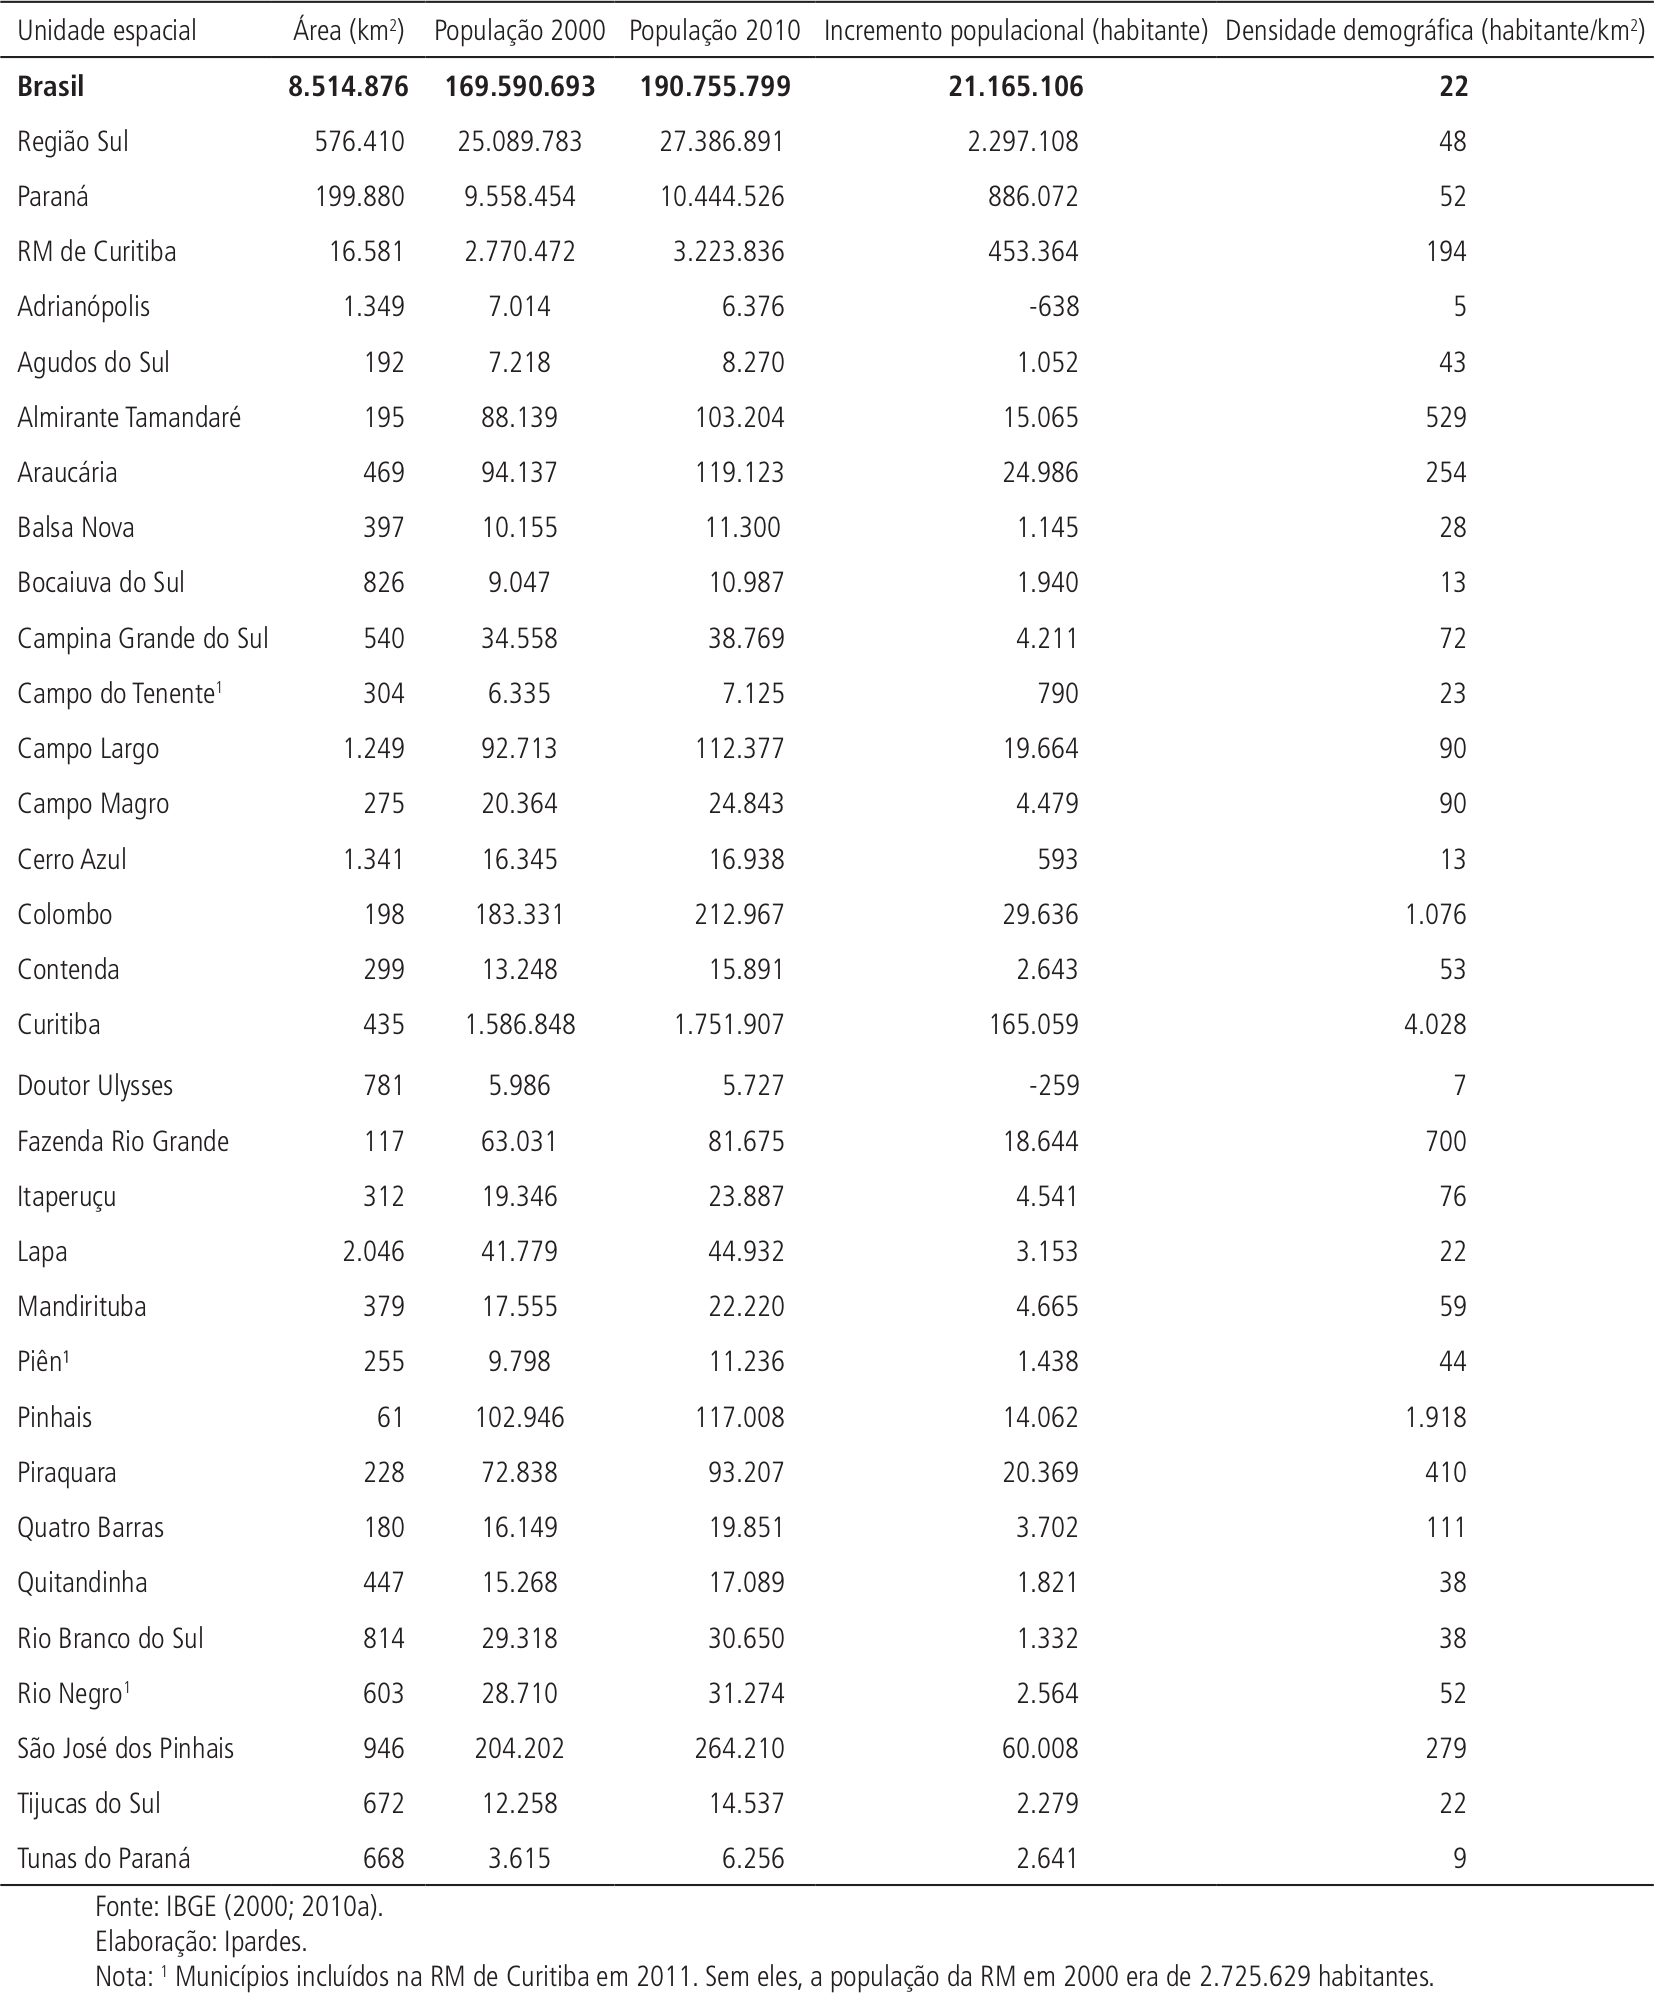
\includegraphics[width=1.0\linewidth]{img/costa2015a_10}
		\label{tab:costa2015a_10}
		\legend{Fonte: \citeonline[p. 11]{costa2015a}}
	\end{table}

	Os três maiores \gls{pib}s do Paraná estão concentrados na \glsdesc{rmc} e estes, por sua vez, são os únicos \gls{pib}s paranaenses que estão entre os cinquenta maiores do país \cite[p. 11]{costa2015a}.

	Além disso,  a metrópole é o quarto maior polo industrial de comércios e serviços. São José dos Pinhais, município limítrofe, aparece em na trigésima sétima posição, localizando o polo automotivo e o aeroporto internacional de Curitiba. A seguir, aparece Araucária, na quadragésima posição, tendo o município um polo petroquímico e industrial. Apesar disso, a \gls{rmc} ainda possui um \gls{pib} per capita abaixo da média do país, da região e do estado \cite[p. 11]{costa2015a}.
	
	Segundo o estudo do Regic, de 2008, a área de influência de Curitiba abrange 666 municípios, possuindo cerca de 16 milhões de pessoas, capilarizando-se no Paraná e em Santa Catarina \cite[p. 16]{costa2015a}. Esta influência é representada cartograficamente na \autoref{fig:costa2015a_11}.
	
	\begin{figure}
		\centering
		\caption{Rede da região Sul (Regic 2012)}
		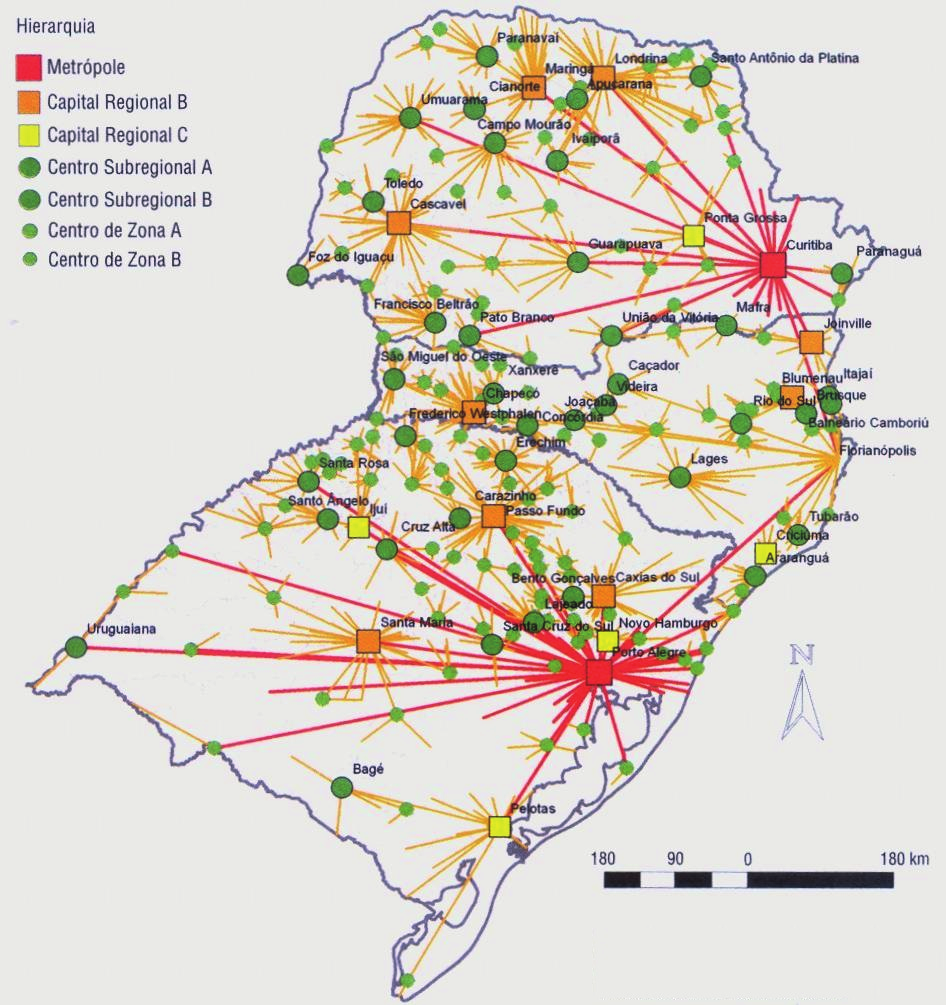
\includegraphics[width=1.0\linewidth]{img/costa2015a_11}
		\label{fig:costa2015a_11}
		\legend{Fonte: \citeonline[p. 11]{costa2015a}}
	\end{figure}
	
	\begin{citacao}
		``A extensão da polarização de Curitiba, abrangendo todo o território do Paraná, e a extrapolação para territórios de estados vizinhos, em especial Santa Catarina, consolidam a centralidade regional da RM de Curitiba e demonstram a dimensão dessa polarização. Tal condição indica que, além de população e riqueza, concentra funções econômicas superiores, bem como uma posição de centro de poder, de decisão e de gestão.'' \apud{rodrigues2009a}{costa2015a}
	\end{citacao}
	
	\subsection{Desigualdades Socioeconômicas}
	% reescrito por Michele
	
	Segundo demonstrado por \citeonline[p. 17]{costa2015a} em seu relatório de pesquisa, as distâncias mais curtas e a inclusão dos municípios na RM não bastaram para que as desigualdades sociais também se encurtasse. Pelo contrário, o caráter concentrador de Curitiba permanece, sua taxa de pobre está em torno de 8\%, enquanto que para os demais integrantes do \gls{nuc} variam de 14\% a 35\%. E isso fica mais preocupante ao se olhar para os municípios que não pertencem ao eixo central, apresentando alguns taxa superior a 50\%, como é o caso de Doutor Ulysses. 
	
	O \gls{ipardes} dispõe de um índice que avalia tais dinâmicas, o \gls{ipdm} (\glsdesc{ipdm}), este revela, em 2010, que enquanto Curitiba apresentava um índice de 0,869, o \gls{nuc} 0,679 e os restantes 0,618. Assim, pode-se observar a concentração que ocorre na metrópole e que a conexão dos demais com este não significa que as condições estão sendo tão benéficas assim, por mais que estão melhorando ao longo dos anos, não parece visível que estejam conseguindo se equiparar ao polo e diminuir as distâncias quantitativas e, sobretudo, qualitativas. Ao se observar os municípios que apresentam crescimento expressivo, como São José dos Pinhais e Araucária, é claro que o seus desempenhos não são o bastante para alcançar os índices de Curitiba. Logo, é importante frisar que crescimento econômico não corresponde diretamente a desenvolvimento. É ainda mais evidente essa dinâmica quando se observa a classificação dos municípios paranaense no \gls{ipdm} Enquanto Curitiba aparece como liderança, os demais integrantes da \gls{rmc} sequer aparecem entre os dez primeiros colocados.
	
	Pode-se observar com mais detalhe os valores dos municípios pertencentes a \gls{rmc} na \autoref{tab:costa2015a_09}.
		
	\begin{table}
		\centering
		\caption{IPDM (2009-2010)}
		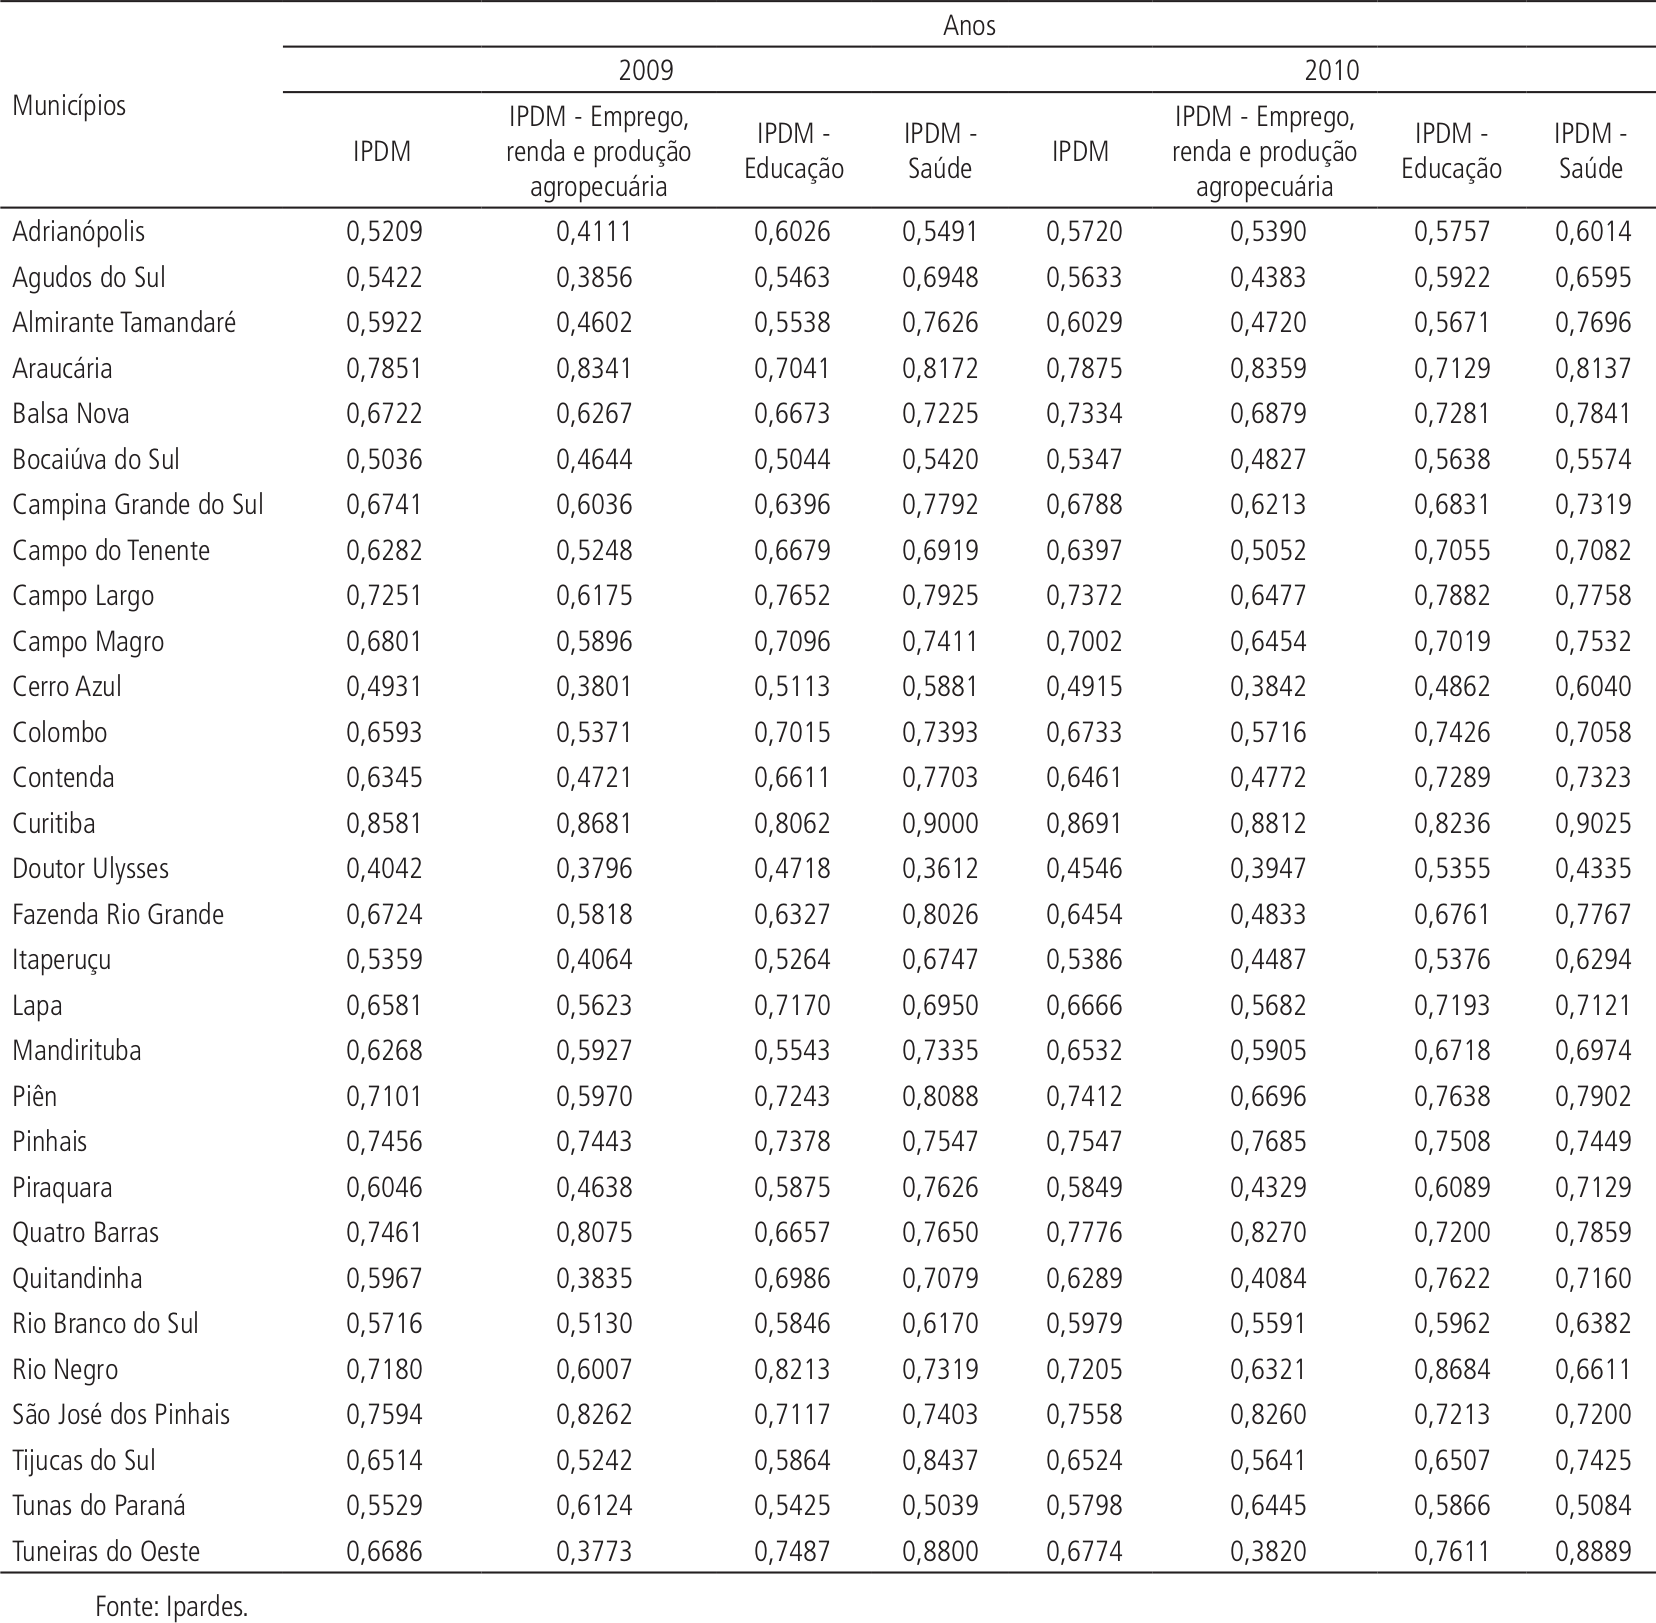
\includegraphics[width=1.0\linewidth]{img/costa2015a_09}
		\label{tab:costa2015a_09}
		\legend{Fonte: \citeonline[p. 17]{costa2015a}}
	\end{table}
	
	\subsection{Ocupação Desordenada}
	% reescrito por Caio, que também acrescentou mais coisas
	
	\subsubsection{Antecedentes - 1950-1960}
	Segundo \citeonline[p. 53]{castro2005a}, Curitiba observa a implementação de seus sistemas viários a partir da Segunda Guerra Mundial, processo este que a favorece como um ``centro de convergência e distribuição de grande parte da produção econômica no estado'' \apud[p. 52]{ipea2001a}{castro2005a}. Na mesma época surgem também (i) o primeiro assentamento precário do município, uma vez que a ocupação urbana fora impulsionada pelo processo de industrialização; e (ii) o planejamento urbano formal, por meio do Plano Agache de 1943, ``que tinha por objetivo definir as diretrizes de crescimento e ordenamento da cidade'', elencando ``o saneamento, o descongestionamento de vias e a definição de áreas para a habitação, serviços e indústrias'' como prioridade \cite[p. 52]{castro2005a}.
	
	No território do que posteriormente viria a ser a \gls{rmc}, observou-se na mesma década um contingente de 210.852 habitantes, fruto principalmente de migrações internas \cite[p. 53]{castro2005a}, no entanto, o crescimento foi maior nos municípios vizinhos entre as décadas de 1940 e 1950, pois estes cresceram 100\% ante 28\% de Curitiba \apud[p. 53]{schussel2001a}{castro2005a}.
	
	Como características do tecido urbano da década de 1950, \apudonline[p. 53]{schussel2001a}{castro2005a} sublinha:
	
	\begin{itemize}
		\item Desenho urbano configurado pela presença da rodovia BR-116 a leste, figurando como barreira;
		\item Presença de algumas manchas isoladas ultrapassando a rodovia BR-116;
		\item Surgimento de 25\% dos lotes legalmente parcelados até a primeira metade da década de 2000;
		\item Adensamento de municípios a leste da \gls{rmc}, nomeadamente São José dos Pinhais, Pinhais e Piraquara, que abrigaram 72\% dos parcelamentos deste período;
		\item Previsão de infraestruturas viárias e de abastecimento em determinadas parcelas do território a leste da \gls{rmc}, como o anel viário denominado Contorno Leste\footnote{Como apontado por \apudonline[p. 53]{schussel2001a}{castro2005a}, ``a demora na execução destas infra-estruturas proporcionou a ocupação urbana irregular nessas áreas''}
	\end{itemize}

	A \autoref{fig:barreiras} espacializa a atual configuração das rodovias e ferrovias, barreiras urbanas em potencial, enquanto a \autoref{fig:br116} espacializa apenas a rodovia BR-116. Os dados foram extraídos da plataforma OpenStreetMap\footnote{Para acessar o sítio do projeto na Internet, acesse \url{https://www.openstreetmap.org/}} a partir do software QGIS, também responsável pelo tratamento.
	
	Como características do tecido urbano na década de 1960, \apudonline[p. 53]{castro2002a}{castro2005a} sublinha a presença de um desenho urbano marcado por duas linhas de descontinuidade, sendo (i) a atual BR-116, que tinha seu efeito barreira reforçado pelo movimento intenso, sendo portanto de difícil transposição; e (ii) a depressão da calha do rio Iguaçu, que sofria inundações periódicas, que impressionavam devido às grandes cavas de exploração de areia.
	
	\begin{landscape}
		\begin{figure}
			\centering
			\caption{Barreiras urbanas potenciais}
			\label{fig:barreiras}
			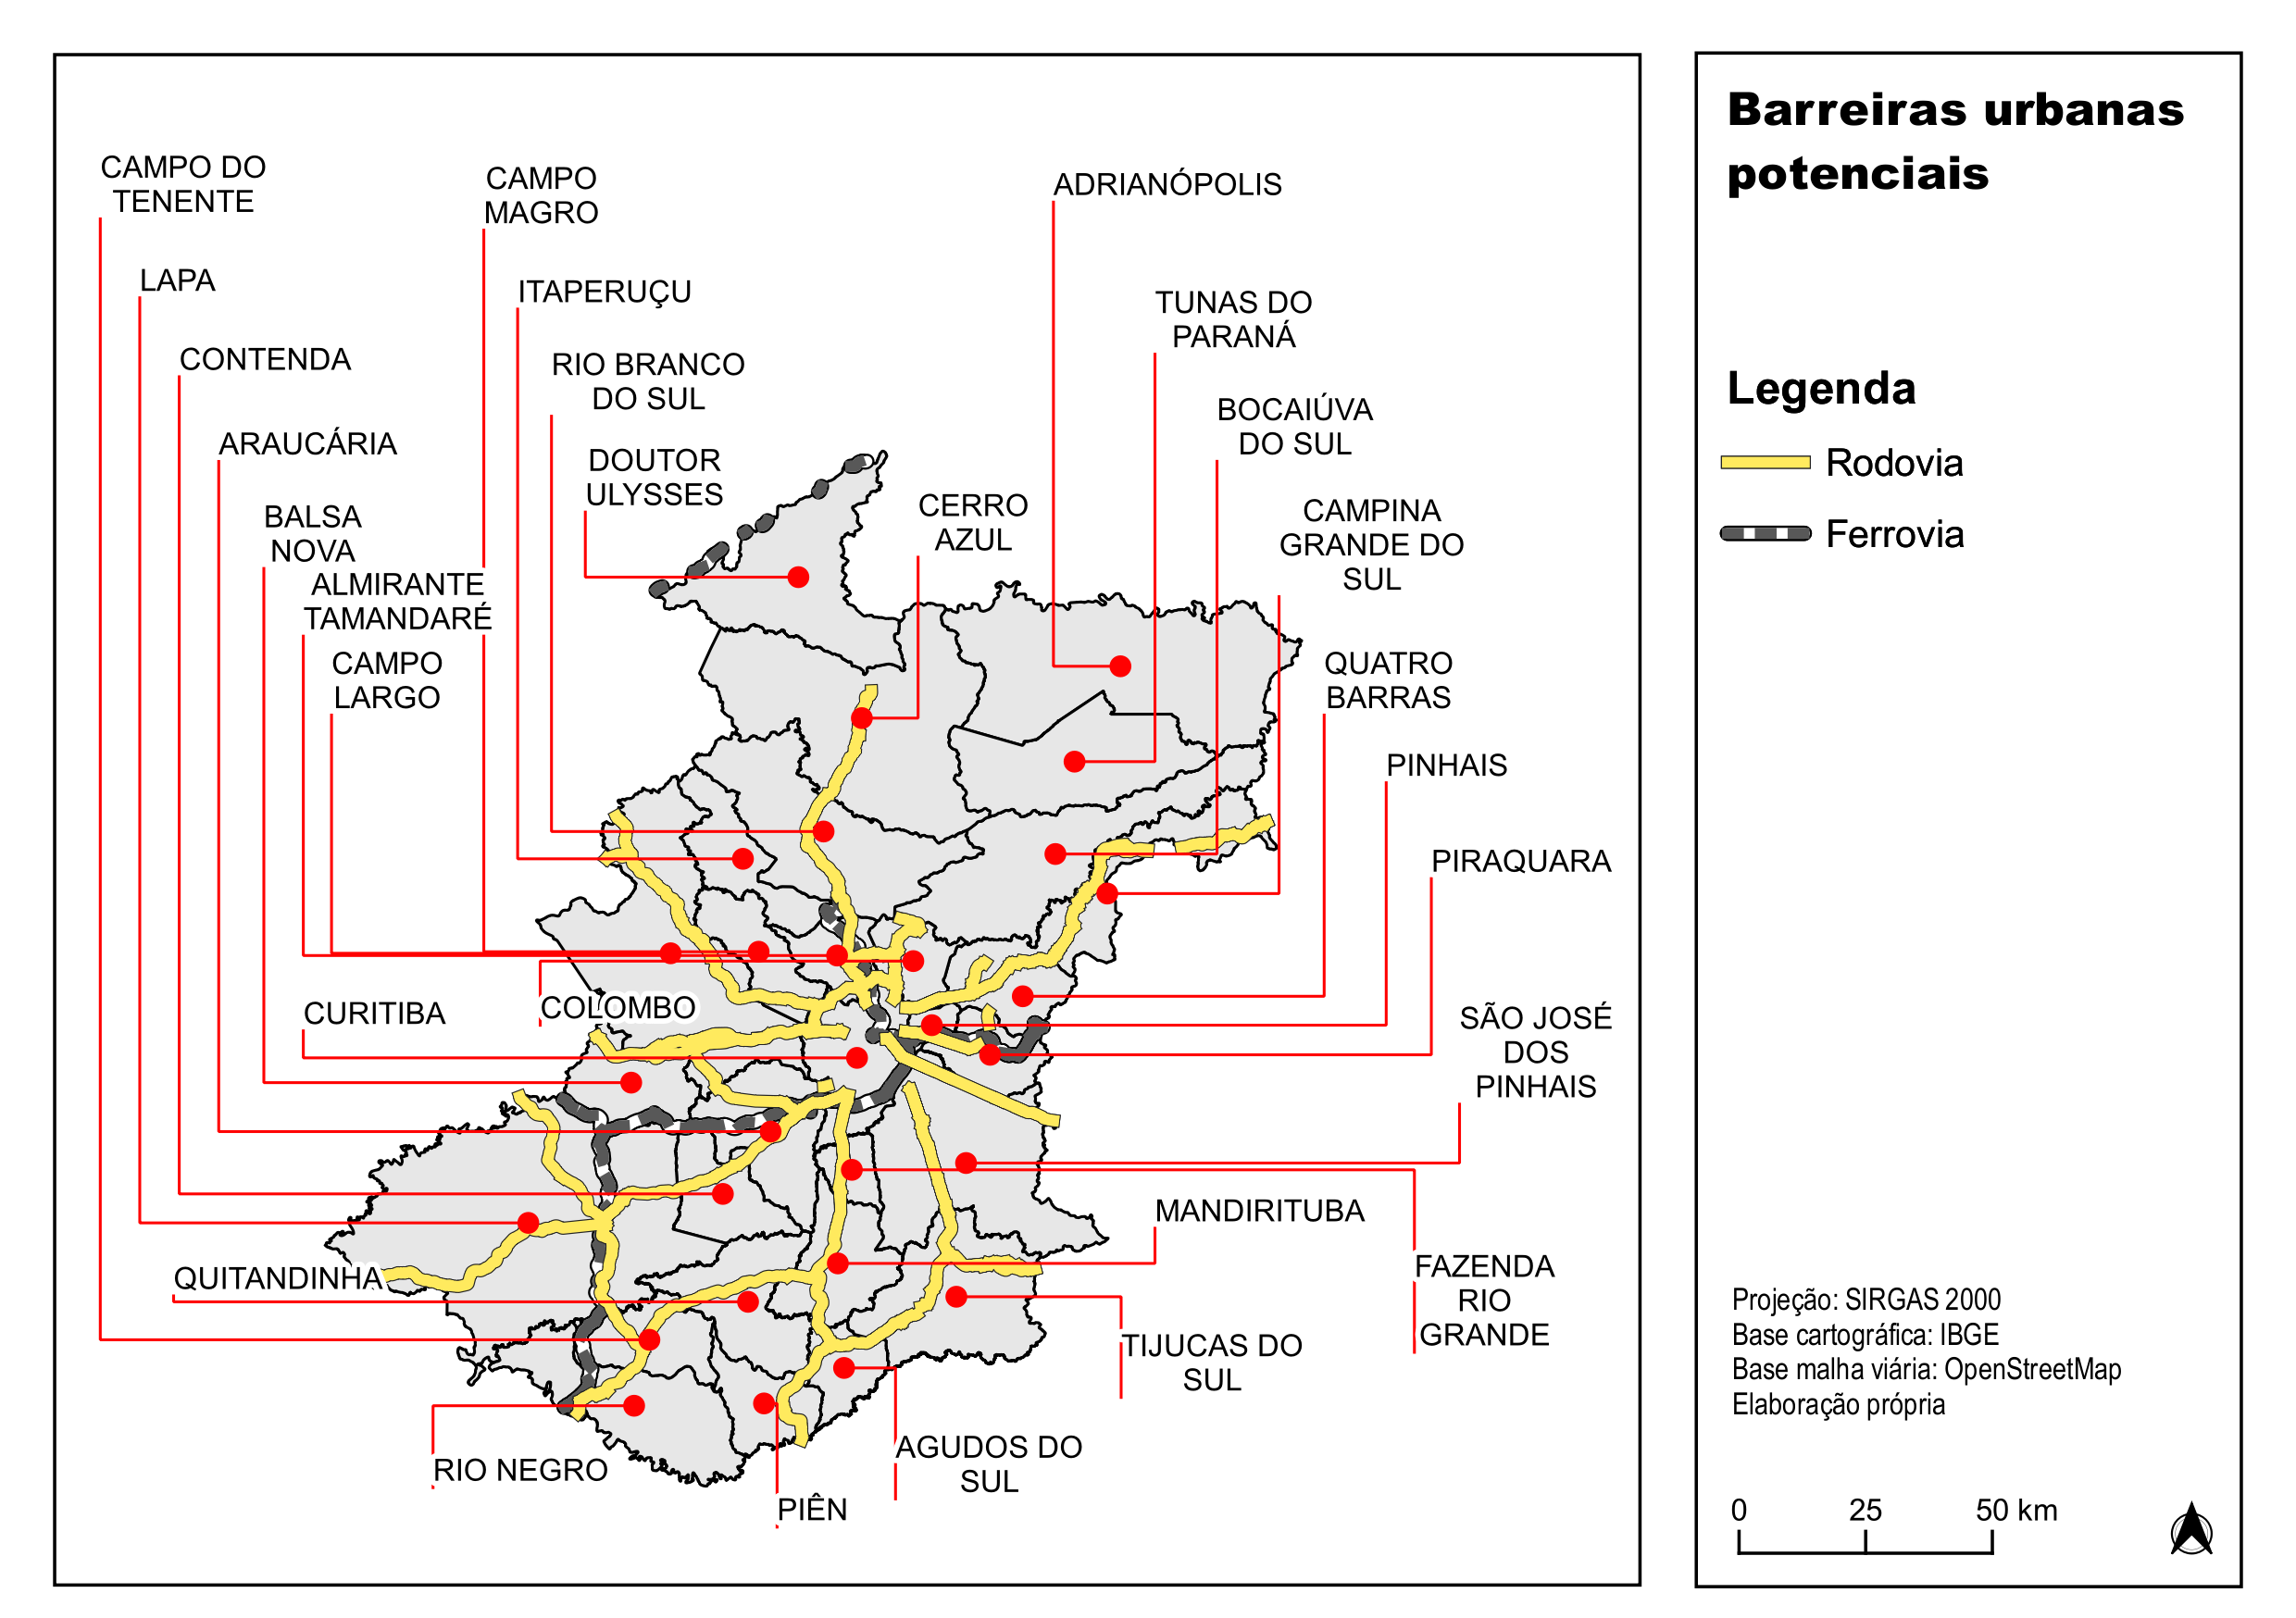
\includegraphics[width=0.85\linewidth]{../gis/produtos/RMC_barreiras}
			\legend{Elaboração própria}
		\end{figure}
	\end{landscape}
	
	\begin{landscape}
		\begin{figure}
			\centering
			\caption{BR-116 como barreira urbana em potencial}
			\label{fig:br116}
			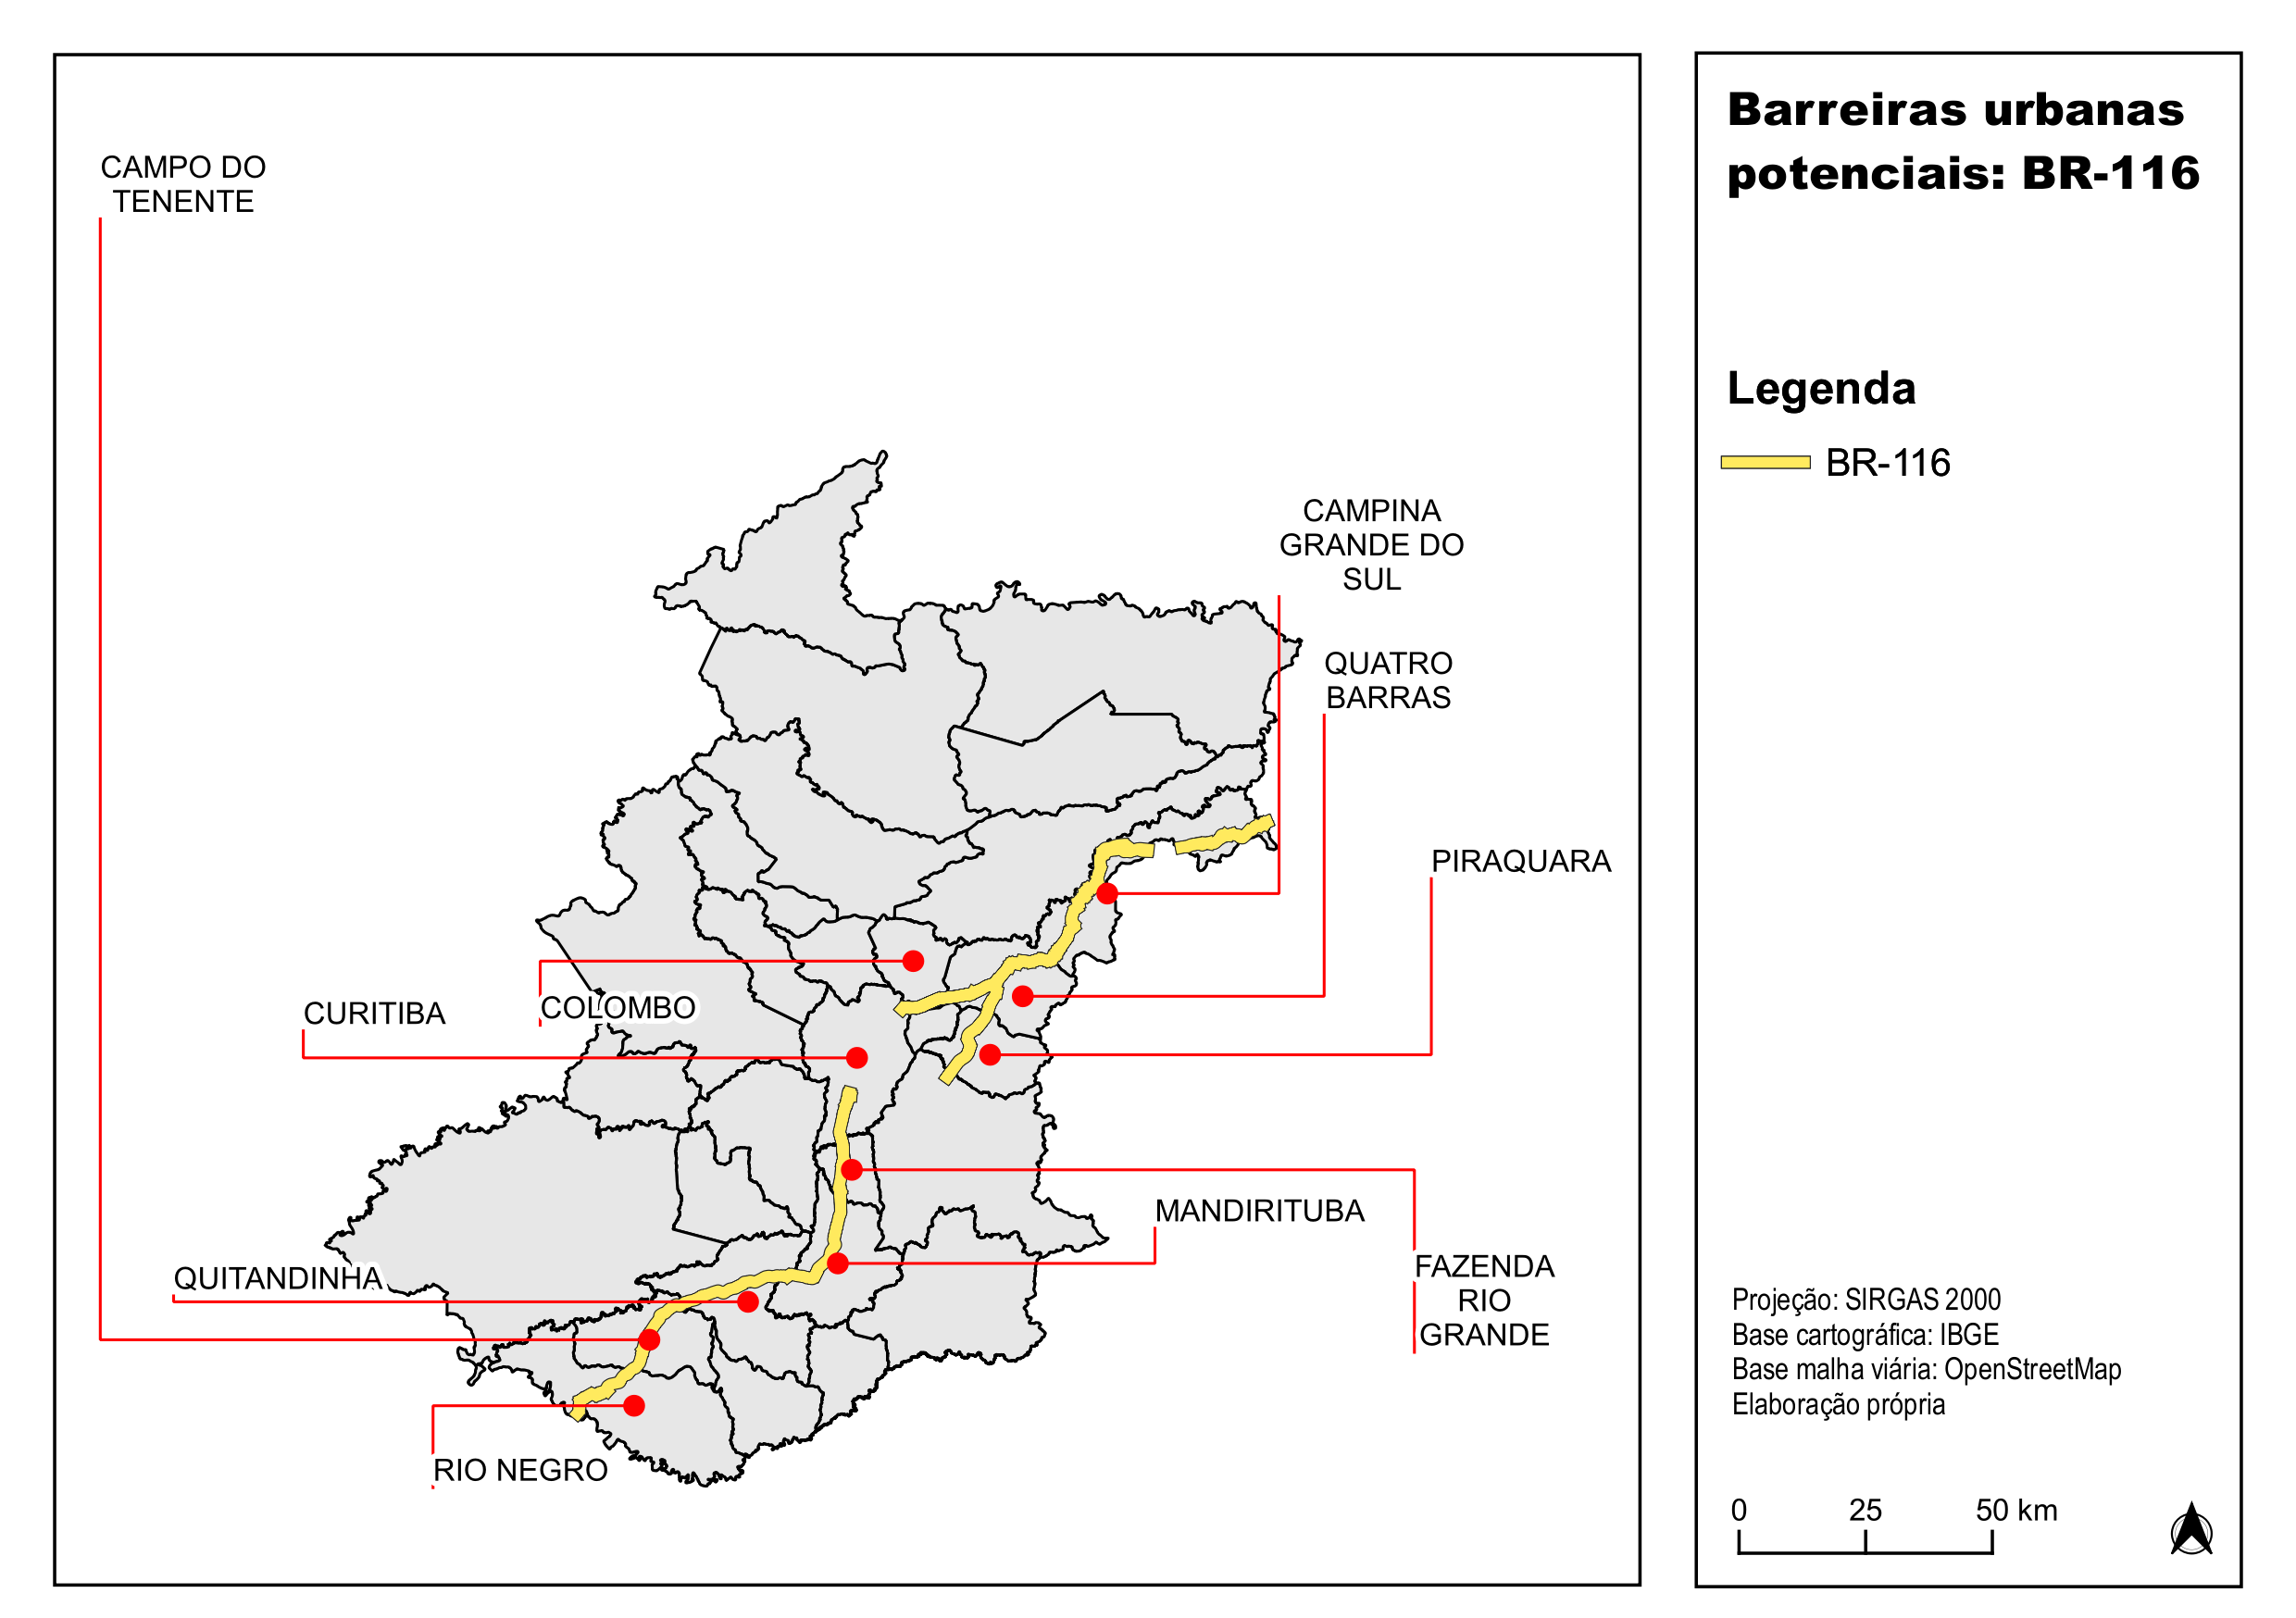
\includegraphics[width=0.85\linewidth]{../gis/produtos/RMC_barreiras_BR116}
			\legend{Elaboração própria}
		\end{figure}
	\end{landscape}
	
	\subsubsection{Antecedentes - 1970-1980} \label{sec:ocup1970}

	No bojo da elaboração do \gls{pdi} de 1978, começa a ser implantada a malha viária do município em conjunto com o Plano Diretor, bem como ações que permitissem o adensamento na envoltória dos eixos rodoviários, consequentemente elevando a demanda de passageiros. \cite[p. 53]{castro2005a}. Trata-se de um plano pioneiro para organização territorial regional, como sublinha \citeonline[p. 138]{lima2001a}, que justifica o pioneirismo elencando a articulação de dados regionais ineditamente analisados sob um recorte metropolitano, que por sua vez definiu diretrizes funcionais que buscava um desenvolvimento sustentável e dinamicamente equilibrado:
	
	\begin{citacao}
		O Plano de Desenvolvimento Integrado da Região Metropolitana de Curitiba – \gls{pdi}, aprovado em 1978, foi o primeiro plano de organização territorial regional e o primeiro produto da Coordenação da Região Metropolitana de Curitiba – Comec, tendo sido elaborado sobretudo porque a instituição oficial da região metropolitana exigia a elaboração de um plano de desenvolvimento da área. De autoria de uma equipe de planejadores, o \gls{pdi} (1978) foi pioneiro na articulação de dados regionais, até então nunca analisados sob o recorte metropolitano, e definiu diretrizes funcionais segundo enfoque sistêmico cujo produto deveria ser uma região equilibrada em suas diferentes dinâmicas, na qual o desenvolvimento urbano tivesse o suporte adequado sem que isso prejudicasse as bases produtivas e a qualidade de vida humana.
	\end{citacao}
	
	O desenvolvimento da malha viária por parte do estado contribuiu para elevar o valor da terra ao longo dos eixos, provocando a ocupação da região leste de Curitiba, com maiores densidades observáveis no vale do rio Iguaçu (bairros Vila Hauer e Boqueirão) e nos municípios de São José dos Pinhais, Pinhais e Piraquara, que se conurbaram \cite[p. 54]{castro2005a}. Ainda segundo \citeonline[p. 54]{castro2005a}, ``ao diluir os limites entre estes municípios, a mancha urbana passou a ocupar áreas cada vez mais periféricas e até mesmo áreas de mananciais de abastecimento de água''.
	
	Segundo \citeonline[p. 137]{lima2001a}, a crise ambiental da \gls{rmc} se torna muito evidente, o que decorre do esgotamento dos mananciais utilizados para abastecimento público de água. Isso se deu devido à expansão da ocupação urbana, estimulada mercadologicamente pelos preços mais baixos dos lotes naquelas regiões, então ``consideradas inadequadas para urbanização'', pois ''compreendem áreas inundáveis e se distribuem na porção sul do município, em zona fronteiriça a outros municípios''.
	
	Uma característica dessa ocupação inadequada é que, para além da expansão da periferia de Curitiba, houve também a construção de loteamentos fora da capital, que nem sempre implantavam uma malha urbana contínua. Estes loteamentos buscavam estar situados próximos dos terminais de transporte coletivo urbano de Curitiba \cite[p. 138]{lima2001a}. A \autoref{fig:terminais}, apresentada posteriormente na \autoref{sec:transportes} (\nameref{sec:transportes}) espacializa os terminais e permite observar que vários destes estão próximos dos limites da capital com os municípios no entorno imediato. Ademais, a lógica dos loteadores estava fundamentada ``no baixo custo da terra e o interesse no usufruto das facilidades urbanas implantadas na capital paranaense'' \cite[p. 138]{lima2001a}.
	
	% TODO parei aqui, dar continuidade às correções sem depender do restante do grupo
	
	
	Fundamentava-se o plano em um modelo de organização territorial, visando a ação metropolitana segundo estratégia intra-regional que previa áreas de contenção, de preservação, de promoção e de dinamização, definidas através da consideração de características e potencialidades do espaço e das atividades existentes. Quanto às áreas dos mananciais de abastecimento público mais importantes para a região, o documento indica que “os centros urbanos nos municípios de Piraquara e São José dos Pinhais deverão ter seus crescimentos controlados de forma mais rígida em virtude de sua localização específica, muito próximos a áreas de captação de água e área inundáveis” (Comec, 1999a:22) e determinava para este vetor leste, ou “subsistema leste”, a estratégia de preservação ambiental, no sentido de conservação. 
	
	No chamado subsistema leste, de acordo com as características físico-geográficas e a ocupação existente e prevista, em decorrência de loteamentos aprovados nas décadas anteriores a 50, o PDI/78 considerava que “o posicionamento geográfico de Curitiba, nas cabeceiras do Rio Iguaçu, bem como dos maiores assentamentos urbanos da região, impede que o desenvolvimento urbano seja orientado na direção leste, área de terrenos planos, sob a pena de esgotar importantes reservas de abastecimento de água. Ao sul o crescimento é limitado pelo Rio Iguaçu e suas áreas de inundações. Ao norte, por uma topografia bastante ondulada. Portanto, o desenvolvimento urbano da região é orientado para oeste; embora estas áreas abriguem terrenos medianamente ondulados, oferecem possibilidades de, desviando os obstáculos, condicionar o crescimento de maneira orgânica.
	
	Segundo dados da Comec, desde períodos anteriores a 1950, estendendo-se até 1994, foram aprovados regularmente 229.618 lotes na RMC. Nos anos 50, verificou-se o efetivo início do processo de parcelamento do solo regional, e de forma bastante expressiva, atingindo cerca de 33\% do total de lotes aprovados na RMC até 1994. Os anos 50 confirmam a constatação anterior em relação à ocupação regional deflagrada na área de mananciais leste,  houve uma explosão na quantidade de lotes aprovados em vários municípios metropolitanos na década de 50, sendo que os maiores números envolvem áreas dos mananciais do leste regional (66,52\%).
	
	Desde as origens do tipo de parcelamento aqui focalizadas na RMC, os municípios do leste metropolitano que contêm em seus territórios os mananciais mais importantes para abastecimento regional – Pinhais, Piraquara e São José dos Pinhais – tiveram um desempenho determinante para tornar significativo este processo. No entanto, ao mesmo tempo, incorporaram a seus territórios elementos potenciais para uma ocupação incompatível com valores ambientais. A aprovação de loteamentos dispersos, desconectados da malha urbana estabelecida, era prática realizada sem parâmetros para avaliação dos danos sociais, econômicos e ambientais futuros.
	
	\begin{figure}
		\centering
		\caption{Comparativo do Total de Lotes Aprovados na Região Metropolitana de Curitiba e Municípios dos Mananciais do Leste Metropolitano (1950-59)}
		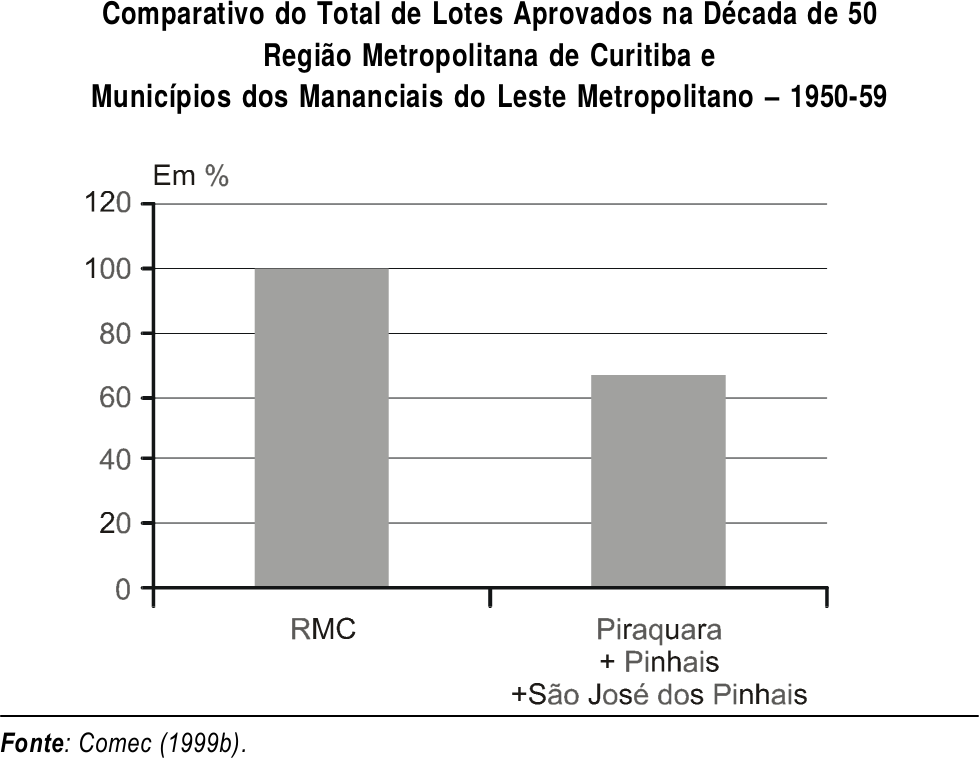
\includegraphics[width=0.6\linewidth]{img/lima2001a_01}
		\label{fig:lima2001a_01}
		\legend{Fonte: \citeonline[p. 140]{lima2001a}}
	\end{figure}

	% TODO continua o plágio de Lima e Mendonça lima2001a
	Na década de 60, na Região Metropolitana de Curitiba, aprovou-se metade do total de lotes da década anterior. Em relação à proteção dos mananciais, o governo estadual da época procedeu à desapropriação de loteamentos aprovados em margens de rios, o que desestimulou a ocupação. Na década 70, sobressai o caráter definitivo de aceleração da ocupação periférica regional, através dos destaques absolutos de número de lotes aprovados nos municípios de Almirante Tamandaré e Colombo, em locais ambientalmente inadequados e desprovidos de estruturação urbana. Tal situação assumiu papel determinante no quadro dos problemas regionais 20 anos depois.
	
	No geral, observa-se uma dinâmica regional de ocupação bastante intensa e que vem se acelerando, com uma taxa de crescimento populacional regional em torno de 3,43\% a.a., enquanto a população do Estado está crescendo 1,24\% (IBGE, 1991 e 1996).
	
	Os recursos hídricos da RMC são limitados e seu esgotamento está próximo, num horizonte de 35 anos. Por outro lado, a necessidade de habitação segue aumentando, ao longo das décadas, no compasso do crescimento populacional, tanto vegetativo quanto de migrações, estas últimas fruto principal da disseminação de uma imagem de cidade sem problemas, com excelente qualidade de vida e com forte poder de atratividade. A questão da contaminação dos mananciais de abastecimento público de água está estreitamente vinculada à realidade econômica e social e depende da capacidade de atendimento às demandas públicas e da mobilização do Estado, ou seja, a efetividade de políticas públicas.
	
	A várzea do Rio Palmital vem sendo progressivamente ocupada de forma irregular desde os anos 70, transformando-se num grande foco de contaminação dos mananciais usados no abastecimento regional público de água. Essa contaminação é causada, dentre outros motivos, pela ocupação conhecida por “Zumbi dos Palmares”, localizada no município de Colombo, que é uma das três maiores ocupações regionais apresentando mais de 1.000 unidades de sub habitações em 1997, segundo Comec, ou seja, uma população de cerca de 3.800 habitantes assentados, sem infra-estrutura, sobre o leito de inundação do rio. 
	
	Entre 1992 e 1997, o número de ocupações irregulares nos municípios do leste enfocados no trabalho – Pinhais, Piraquara e São José dos Pinhais – cresceu cerca de 4,5 vezes em cinco anos, o que pode significar que, a cada ano, instalaram-se precariamente nestes municípios cerca de 5.783 pessoas ou, a cada dia, mais de 15 pessoas, ou quatro famílias, considerando uma média regional de componentes da unidade familiar. Este valor atinge, em 1997, um total de 38.221 pessoas, nos três municípios, em estado de carência generalizada, pois as ocupações irregulares normalmente formam um quadro de extrema precariedade, não apenas quanto aos assentamentos em si, na sua materialidade, mas principalmente no que se refere à precariedade física, de formação profissional e da cidadania dos seus moradores.
	
	Finalmente, dadas as considerações de \apudonline[p. 3]{andreoli1992a}{andreoli1999a}, faz-se necessário pontuar a existência de uma fronteira agrícola nas regiões oeste e sudeste do Paraná, que expandiu-se aceleradamente entre as décadas de 1950 e 1970 devido à implantação de sistemas agrícolas imediatistas. O resultado da expansão em questão foi uma degradação ambiental contínua e progressiva, sumarizada por \citeonline[p. 3--4]{andreoli1999a} como se segue:
	
	\begin{citacao}
		Este processo de expansão da fronteira agrícola, realizado visando o lucro imediato não se preocupou com o correto manejo do solo, com isso as formas inadequadas de preparo do solo provocaram intensos processos erosivos com a remoção da camada mais fértil e degradação física do solo. Esta ação representa a perda do solo pela erosão e o transporte de 12.587.969 toneladas por ano de solos nas principais bacias do Paraná. Segundo dados do Departamento Nacional de Água e Energia Elétrica (DNAEE) os rios que mais contribuem para esta cifra são os rios Ivaí e Paraná que transportam, respectivamente, 2.708.300 e 8.325.504 toneladas de solo por ano.
	\end{citacao}

	A subseção \autoref{sec:franjas} observa dados do Censo Agropecuário 2017 do \glsdesc{ibge} para melhor compreender como a presença de atividades agrícolas e de pecuária se dá na \glsdesc{rmc}.
	
	\subsection{Vocação das franjas rurais - análise do Censo Agropecuário} \label{sec:franjas}
	% análise feita pela Mari
	
	O Censo Agropecuário é um levantamento realizado pelo \gls{ibge} a cada 5 anos, salvas exceções de cortes orçamentários, que visa coletar informações sobre estabelecimentos agropecuários e as atividades neles desenvolvidas. Segundo o IBGE, o censo ``tem como unidade de coleta toda unidade de produção dedicada, total ou parcialmente, a atividades agropecuárias, florestais ou aquícolas, subordinada a uma única administração (produtor ou administrador), independentemente de seu tamanho, de sua forma jurídica ou de sua localização, com o objetivo de produção para subsistência ou para venda''\footnote{Para mais informações e acesso aos resultados do último Censo, veja \citeonline{ibgerural2019a}}.
	
	Nesta subseção, buscamos caracterizar as franjas rurais da \gls{rmc} por meio dos principais dados coletados durante o último censo realizado (2017). Para isto, consideramos como Franja Norte as cidades de Bocaiúva do Sul, Tunas do Paraná, Adrianópolis, Cerro Azul e Doutor Ulysses, e como Franja Sul observamos Tijucas do Sul, Agudos do Sul, Mandirituba, Piên, Rio Negro, Campo do Tenente, Quitandinha, Contenda, Lapa e Balsa Nova.
	
	\subsubsection{Agricultura}
	
	O primeiro dado observado para entendermos as características do setor agropecuário das franjas da \glsdesc{rmc}, foi a quantidade produzida em toneladas por município. Os dados coletados estão representados cartograficamente na \autoref{fig:qtdeagro}.
	
	\begin{landscape}
		\begin{figure}
			\centering
			\caption{Produção da agricultura por município das franjas da \gls{rmc}}
			\label{fig:qtdeagro}
			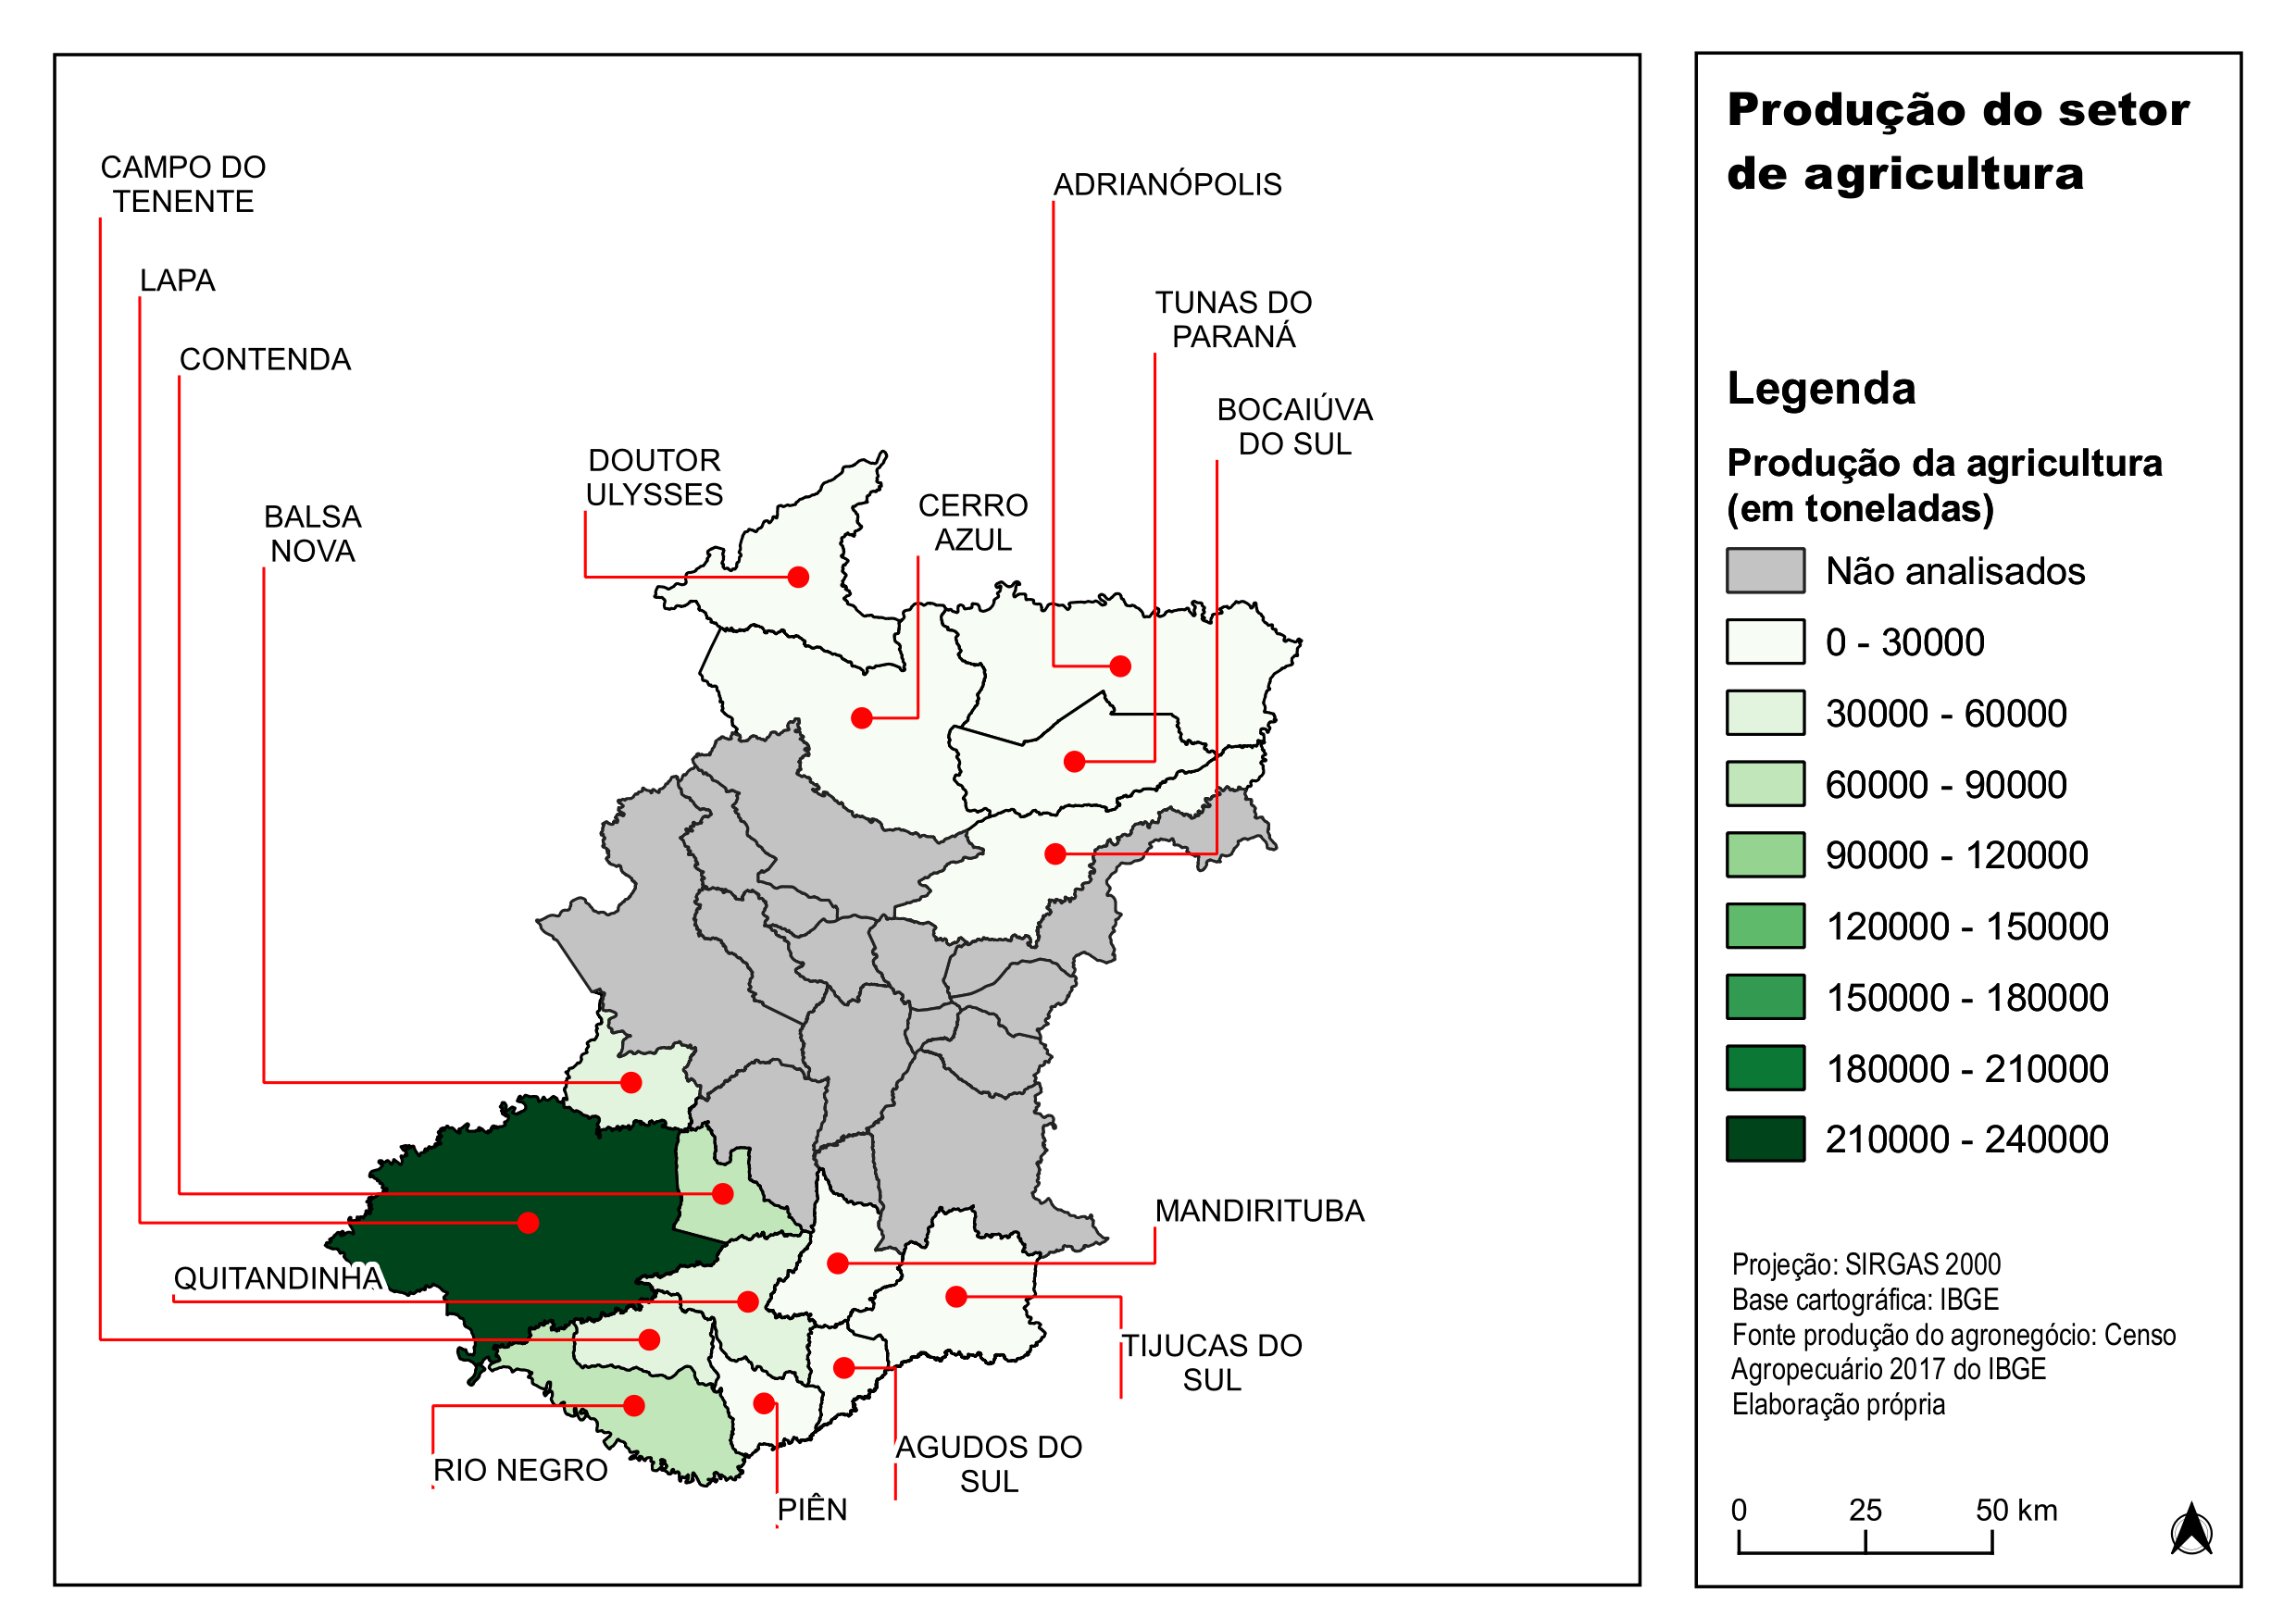
\includegraphics[width=0.85\linewidth]{../gis/produtos/RMC_censorural_QTDE_PRODUZIDA_AGRO}
			\legend{Elaboração própria. Fonte: Censo Agropecuário 2017 do IBGE}
		\end{figure}
	\end{landscape}
	
	É possível notar a partir da \autoref{fig:qtdeagro} a grande diferença no total absoluto produzido por cada uma das franjas. A Franja Norte produziu, no total, 32.367 toneladas de produtos do setor agropecuário no mesmo período em que a Franja Sul produziu 575.324 toneladas. Podemos explicar esta situação através de dois fatores: o primeiro fator é o total da área destinada a esse tipo de atividade, que foi de 73 km² para Franja Norte e 1.323 km² para Franja Sul. Em análise detalhada no nível município, a correlação entre área ocupada para lavoura e o total de sua produção é de 99.4\%. O segundo fator é a produção média por estabelecimento, que foi de 41,23 toneladas/ano na Franja Sul e 15,69 toneladas/ano na Franja Norte. Este mesmo indicador por município está distribuído conforme a \autoref{fig:qtdeestabagro}.
	
	Analisamos também a quantidade de estabelecimentos que se declaram agropecuários em comparação à área total do município. Desta forma, temos a concentração por quilometro quadrado deste tipo de atividade em cada uma das cidades da RM. Trata-se de uma dinâmica que foi espacializada na \autoref{fig:qtdekmagro}.
	
	Pode-se notar que, como esperado, no geral, os municípios da Franja Sul possuem uma concentração maior de estabelecimentos agropecuários por quilometro quadrado. Consolidando os números por franja, enquanto a Franja Sul possui 1.79 estabelecimentos/km², a Franja Norte possui, na média, 2.73 estabelecimentos/km². 
	
	Quanto ao tipo de produto que cada uma das regiões possui, analisamos a quantidade produzida nas lavouras temporárias, que representam 99\% da manufatura de acordo com os dados coletados pelo IBGE. Tem-se a configuração organizada na \autoref{tab:rural_A}:
	
	\begin{landscape}
		\begin{figure}
			\centering
			\caption{Produção da agricultura por estabelecimento das franjas da \gls{rmc}}
			\label{fig:qtdeestabagro}
			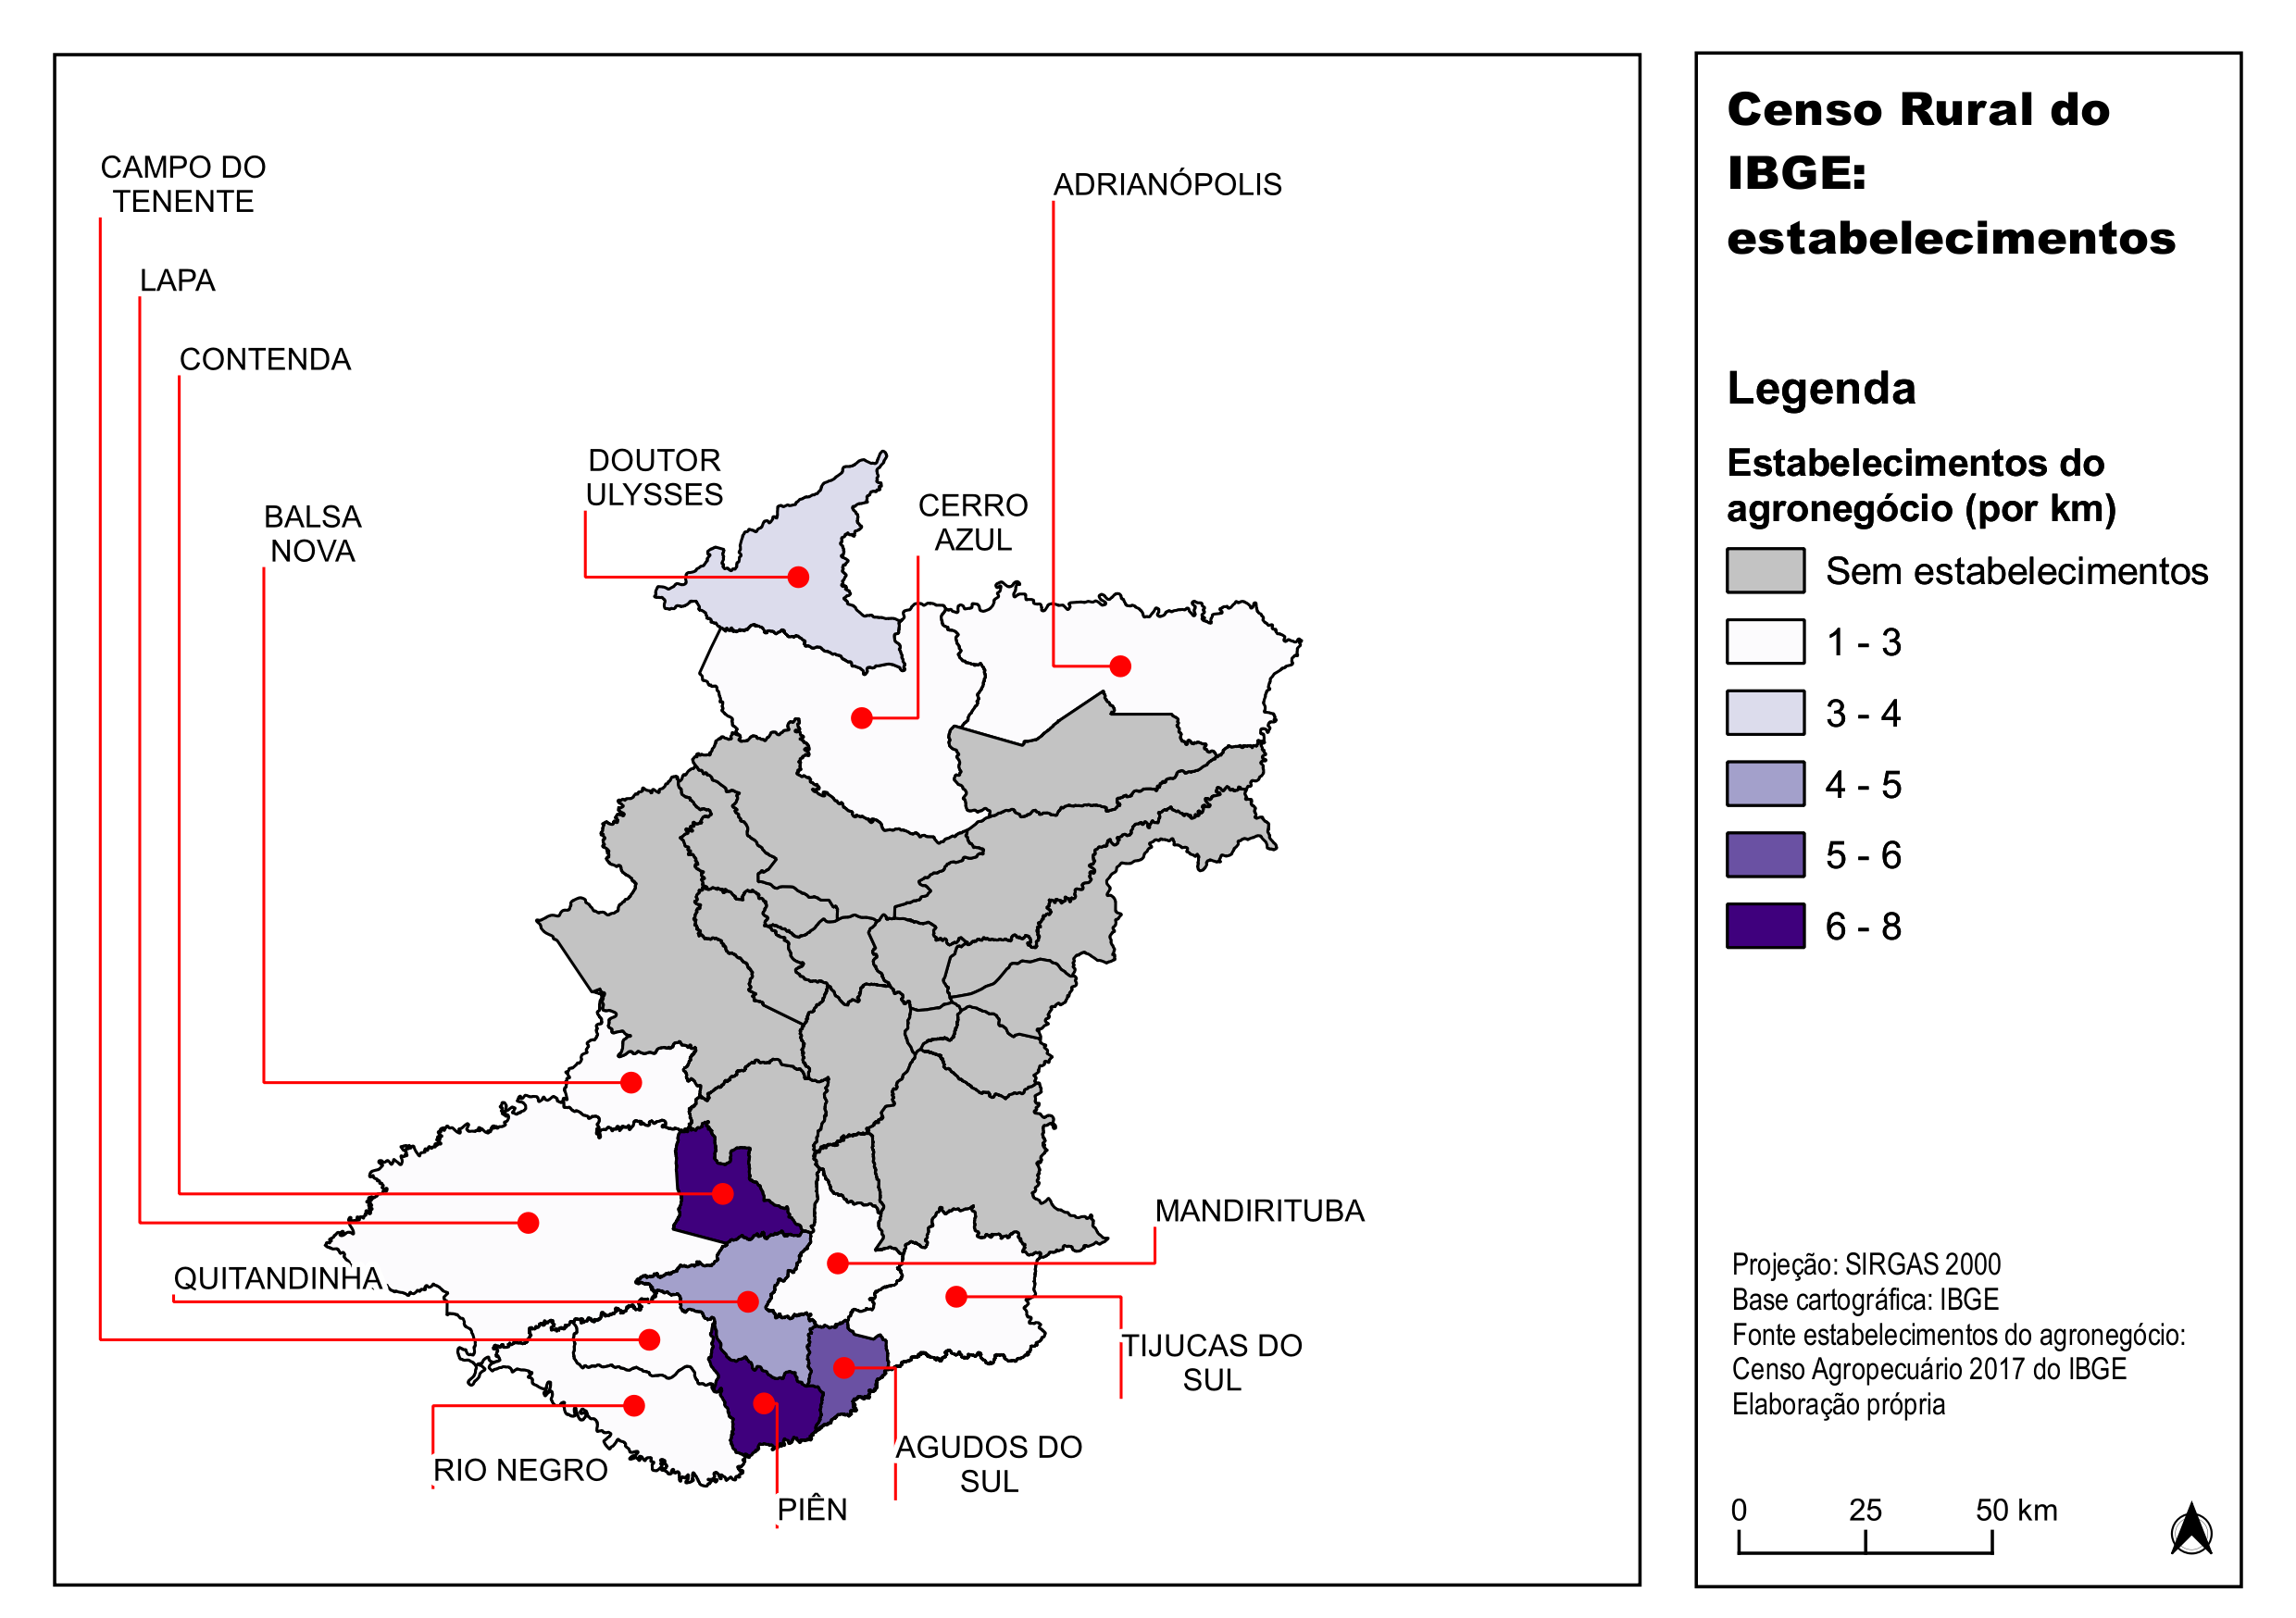
\includegraphics[width=0.85\linewidth]{../gis/produtos/RMC_censorural_QTD_ESTAB_AGRO}
			\legend{Elaboração própria. Fonte: Censo Agropecuário 2017 do IBGE}
		\end{figure}
	\end{landscape}
	
	\begin{landscape}
		\begin{figure}
			\centering
			\caption{Estabelecimentos de agricultura por km das franjas da \gls{rmc}}
			\label{fig:qtdekmagro}
			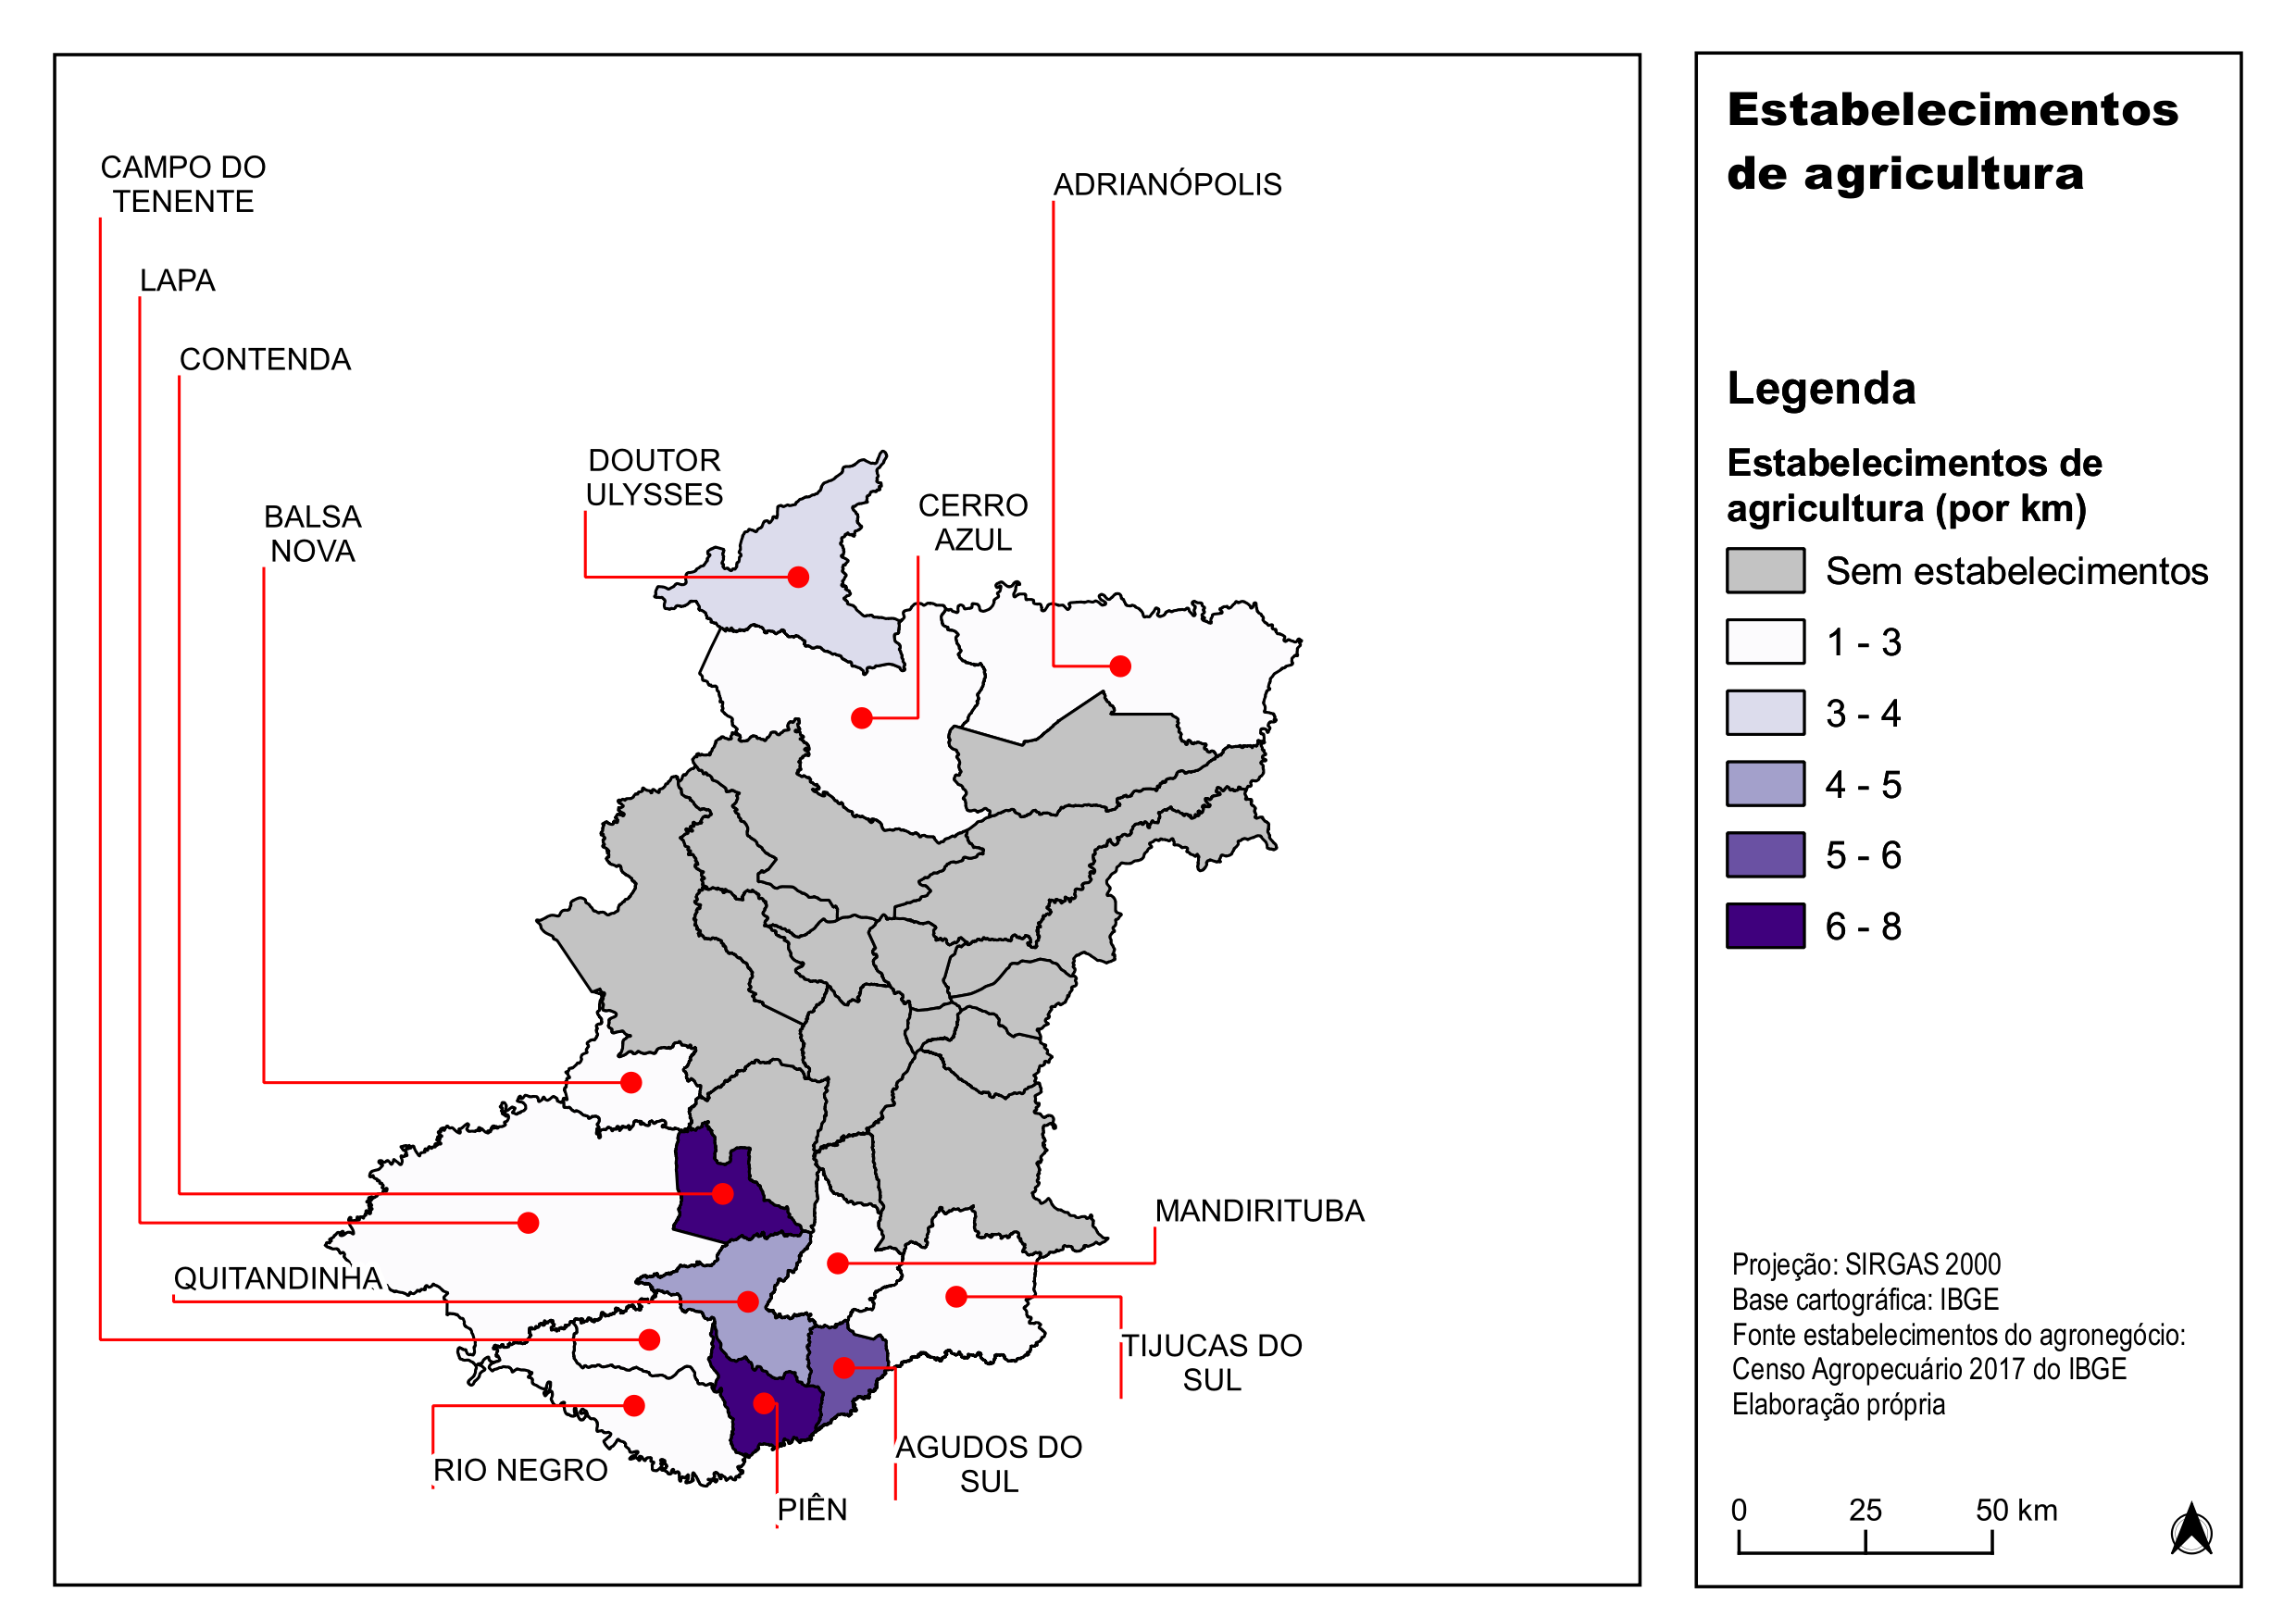
\includegraphics[width=0.85\linewidth]{../gis/produtos/RMC_censorural_QTD_ESTAB_KM_AGRO}
			\legend{Elaboração própria. Fonte: Censo Agropecuário 2017 do IBGE}
		\end{figure}
	\end{landscape}
	
	\begin{table}
		\centering
		\caption{Produtos por franja da \gls{rmc}}
		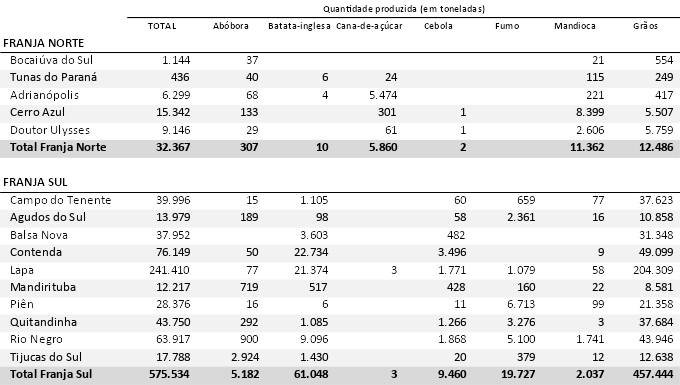
\includegraphics[width=1\linewidth]{img/rural_A}
		\label{tab:rural_A}
		\legend{Elaboração própria. Fonte: Censo Agropecuário 2017 do IBGE}
	\end{table}

	Pela \autoref{tab:rural_A} é possível perceber as diferenças nos produtos das lavouras temporárias por franja. Na Franja Sul, a produção de grãos como aveia, milho, trigo, feijão e principalmente soja representam 77.5\% do total manufaturado, enquanto para Franja Norte este número cai para 57.2\%, sendo que em Adrianópolis ele chega a apenas 6.6\%. Outras produções relevantes para a Franja Sul são as da batata (8.1\%) e do fumo (6.2\%), mas não chegam nem perto da representatividade da lavoura dos grãos.

	A Franja Norte possui sua manufatura um pouco menos concentrada em relação à Franja Sul. Apesar de, como falado anteriormente, ter 57.2\% de lavoura voltada aos grãos, as produções de mandioca e cana-de-açúcar são responsáveis por 23\% e 19\% respectivamente, sendo que o município que concentra a manufatura da cana é Adrianópolis e a mandioca são Cerro Azul e Doutor Ulysses.
	
	\subsubsection{Pecuária}
	
	Assim como no setor da Agricultura, iniciamos a análise da Pecuária nas franjas da Região Metropolitana de Curitiba através da quantidade produzida (cabeças) por município. A série de dados apresenta a distribuição expressa cartograficamente na \autoref{fig:qtdepec}.
	
	\begin{landscape}
		\begin{figure}
			\centering
			\caption{Produção da pecuária por município das franjas da \gls{rmc}}
			\label{fig:qtdepec}
			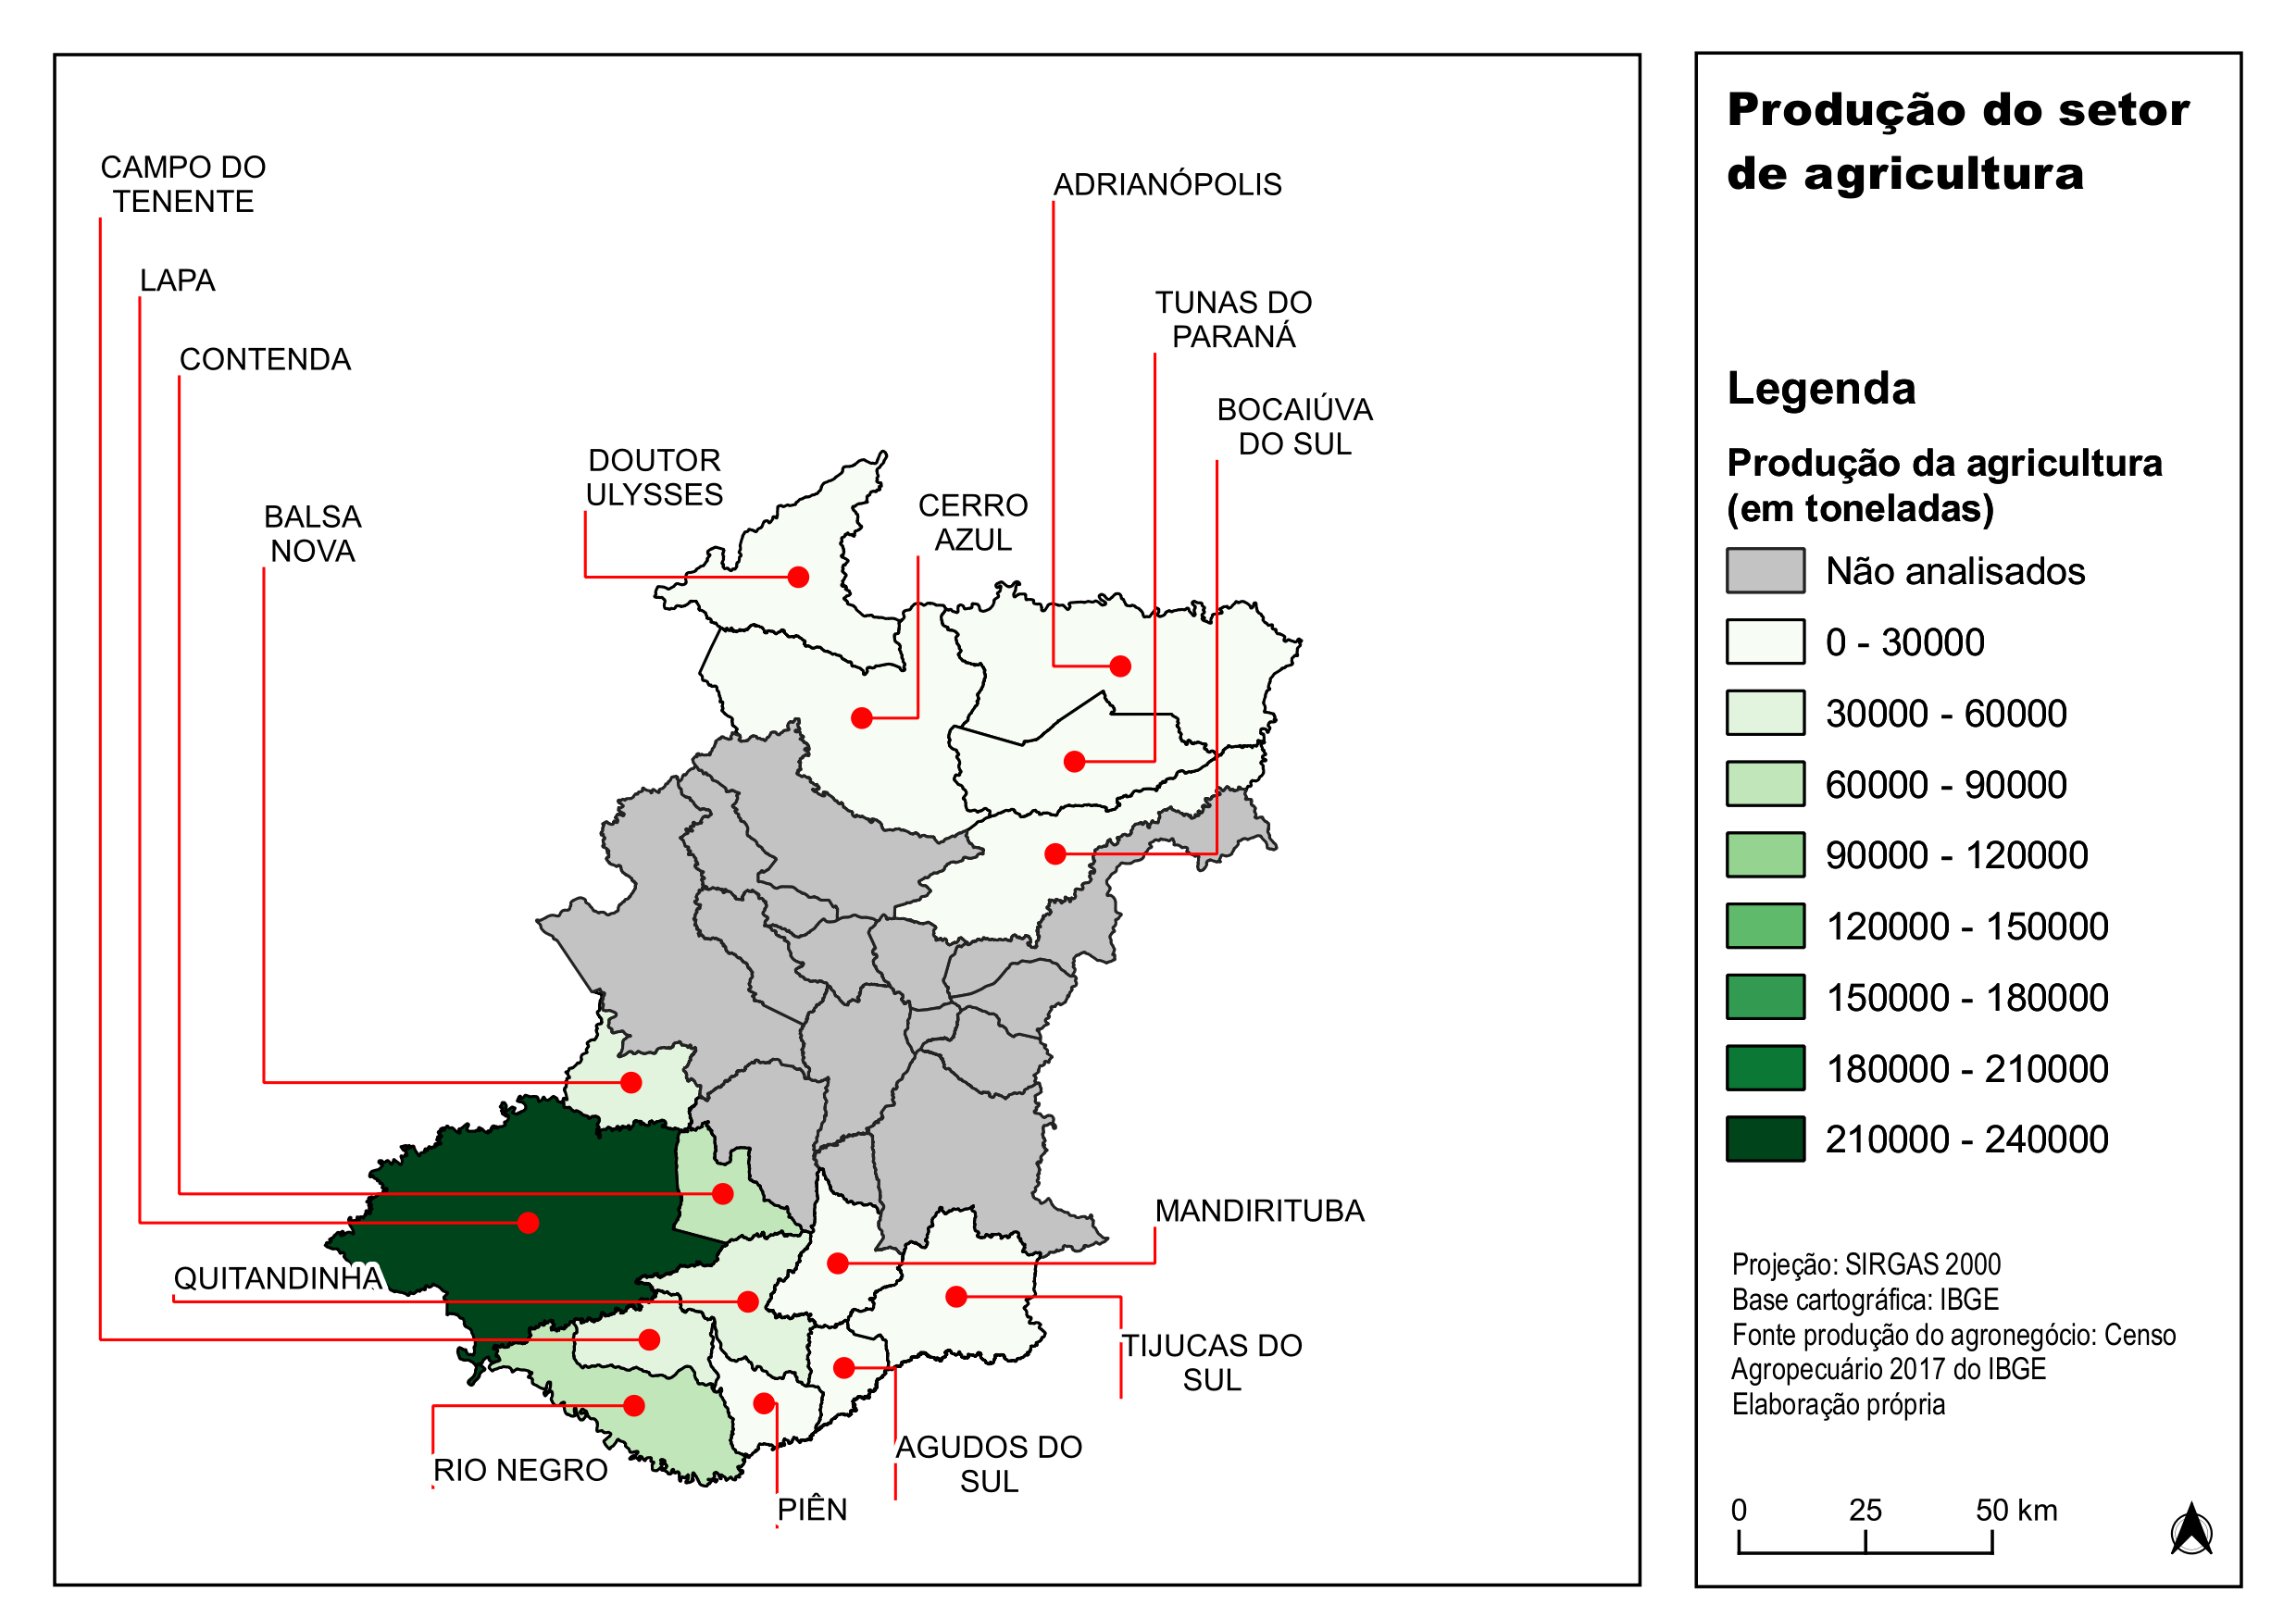
\includegraphics[width=0.85\linewidth]{../gis/produtos/RMC_censorural_QTDE_PRODUZIDA_AGRO}
			\legend{Elaboração própria. Fonte: Censo Agropecuário 2017 do IBGE}
		\end{figure}
	\end{landscape}

	\begin{landscape}
		\begin{figure}
			\centering
			\caption{Produção da pecuária por estabelecimento das franjas da \gls{rmc}}
			\label{fig:qtdeestabpec}
			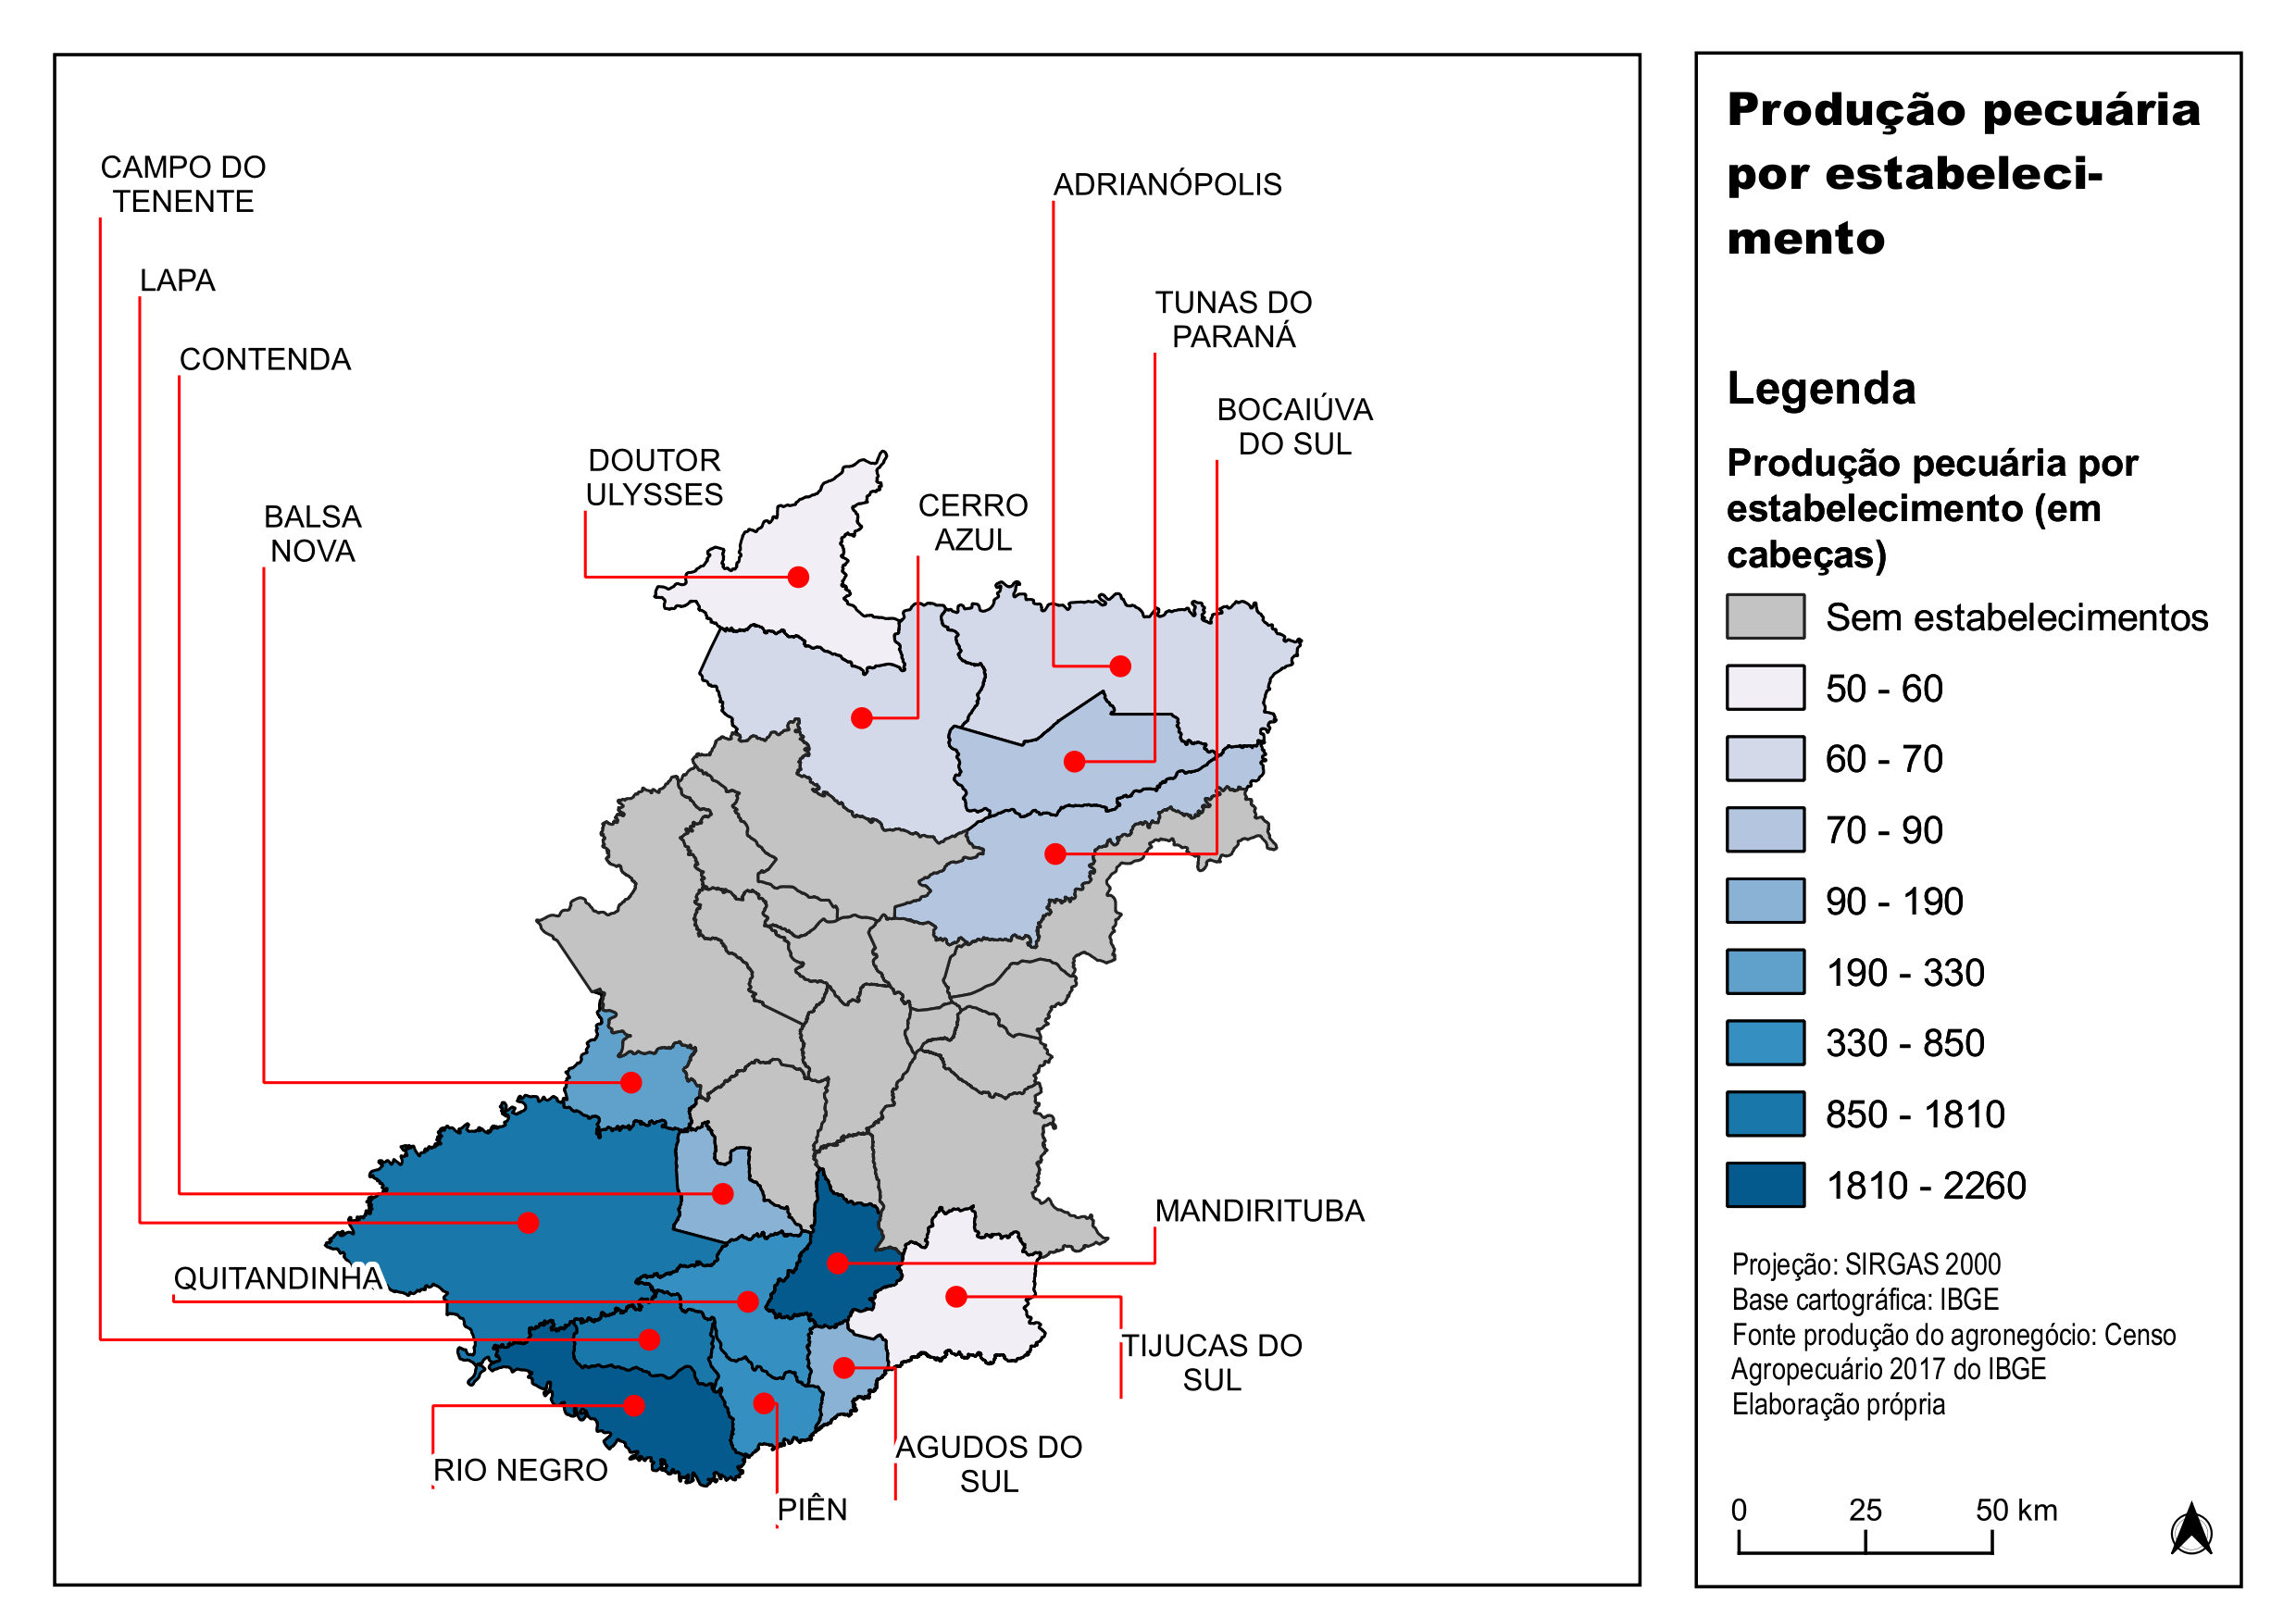
\includegraphics[width=0.85\linewidth]{../gis/produtos/RMC_censorural_QTD_ESTAB_PEC}
			\legend{Elaboração própria. Fonte: Censo Agropecuário 2017 do IBGE}
		\end{figure}
	\end{landscape}

	Pode-se notar facilmente através do mapa as disparidades entre as quantidades produzidas por franja. A Franja Norte produziu no total 233.832 cabeças, enquanto a Franja Sul produziu 5.582.118. Para este setor, o IBGE não disponibiliza a área total destinada à atividade, e por este motivo não é possível realizar a análise de espaço ocupado por produção. Entretanto, a análise da produção média por estabelecimento mostrou o mesmo resultado do setor da Agricultura: a Franja Norte produziu 66,49 cabeças por estabelecimento, enquanto a Franja Sul produziu 805,85. A \autoref{fig:qtdeestabpec} apresenta um mapa deste indicador por estabelecimento.
	
	Quanto à espécie da pecuária, podemos também notar os mesmos padrões encontrados no setor Agropecuário. A Franja Sul concentra sua produção em uma espécie (aves - 98\%), enquanto a Franja Norte possui uma produção menos centralizada. Tem-se a \autoref{tab:rural_B}.

	\begin{table}[h]
		\centering
		\caption{Quantidade de cabeças produzidas na \gls{rmc}}
		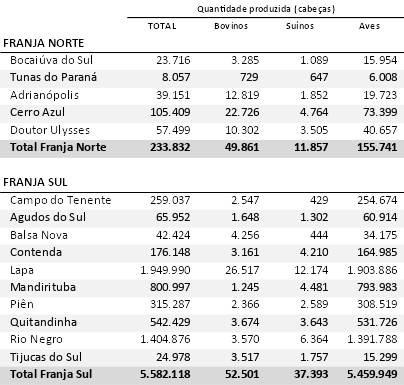
\includegraphics{img/rural_B}
		\label{tab:rural_B}
		\legend{Elaboração própria. Fonte: Censo Agropecuário 2017 do IBGE}
	\end{table}

	Em suma, no setor da Pecuária as conclusões são bastante similares em relação ao setor da Agricultura, tanto em termos de proporções de produção e produtividade, quanto nos municípios relevantes em cada uma das Franjas analisadas.

	\section{Funções públicas de interesse comum}
	% escrito por Mari
	
	As funções públicas de interesse comum (\gls{fpic}s) metropolitanas são provenientes, principalmente, dos artigos 23 e 30 da Constituição Federal de 1988. Segundo \citeonline[p. 145]{cesar2017a}, ``o art. 23 cuida da competência executiva comum, compartilhada por todos os entes federados enquanto o art. 30 trata das competências exclusivas dos municípios, com destaque para seu inciso V, que atribui ao município a organização e prestação, direta ou sob o regime de concessão ou permissão, os serviços públicos de interesse local''.
	
	Entretanto, segundo \cite{barroso2007a}, o interesse local dificilmente será exclusivo de um município. Este é parte de um fenômeno vivo que, com o evoluir dos eventos sociais, aumenta sua abrangência territorial. Neste sentido, a Constituição Federal assente a particularidade das áreas urbanas, e permite a instituição de regiões metropolitanas para que seja feita a correta gestão e o devido planejamento das funções públicas de interesse comum.
	
	Portanto, segundo \citeonline[p. 146]{cesar2017a}, tem-se como objetivo principal da gestão das \gls{fpic}s ``o desenvolvimento econômico e social da região metropolitana, a partilha equilibrada dos seus benefícios e a definição de políticas compensatórias dos efeitos da sua polarização''.
	
	Assim sendo, trataremos nesta seção da caracterização das principais \gls{fpic}s da \glsdesc{rmc}, e, logo em seguida, baseando-se nas situações relevantes retratadas, apresentaremos nossa proposta de gestão.
	
	\subsection{Recursos hídricos e proteção ambiental}
	% escrito por Caio
	
	Segundo \citeonline[p. 427]{kornin2014a}, ``a área de proteção dos mananciais da \gls{rmc} abrange quase todos os municípios metropolitanos'', existindo ainda espaços de conflito na esteira na expansão da mancha urbana da capital e das áreas de entorno direto ao polo, sendo estes associados com ``a urbanização e a necessidade de manutenção da qualidade hídrica e ambiental dos mananciais de abastecimento''. A \autoref{fig:kornin2014a_01} espacializa os corpos hídricos relevantes e os mananciais protegidos nos termos do Decreto Estadual n.º 6.194/12.
	
	\begin{figure}
		\centering
		\caption{Área de proteção dos mananciais da \gls{rmc} (D.E. No 6.194/12)}
		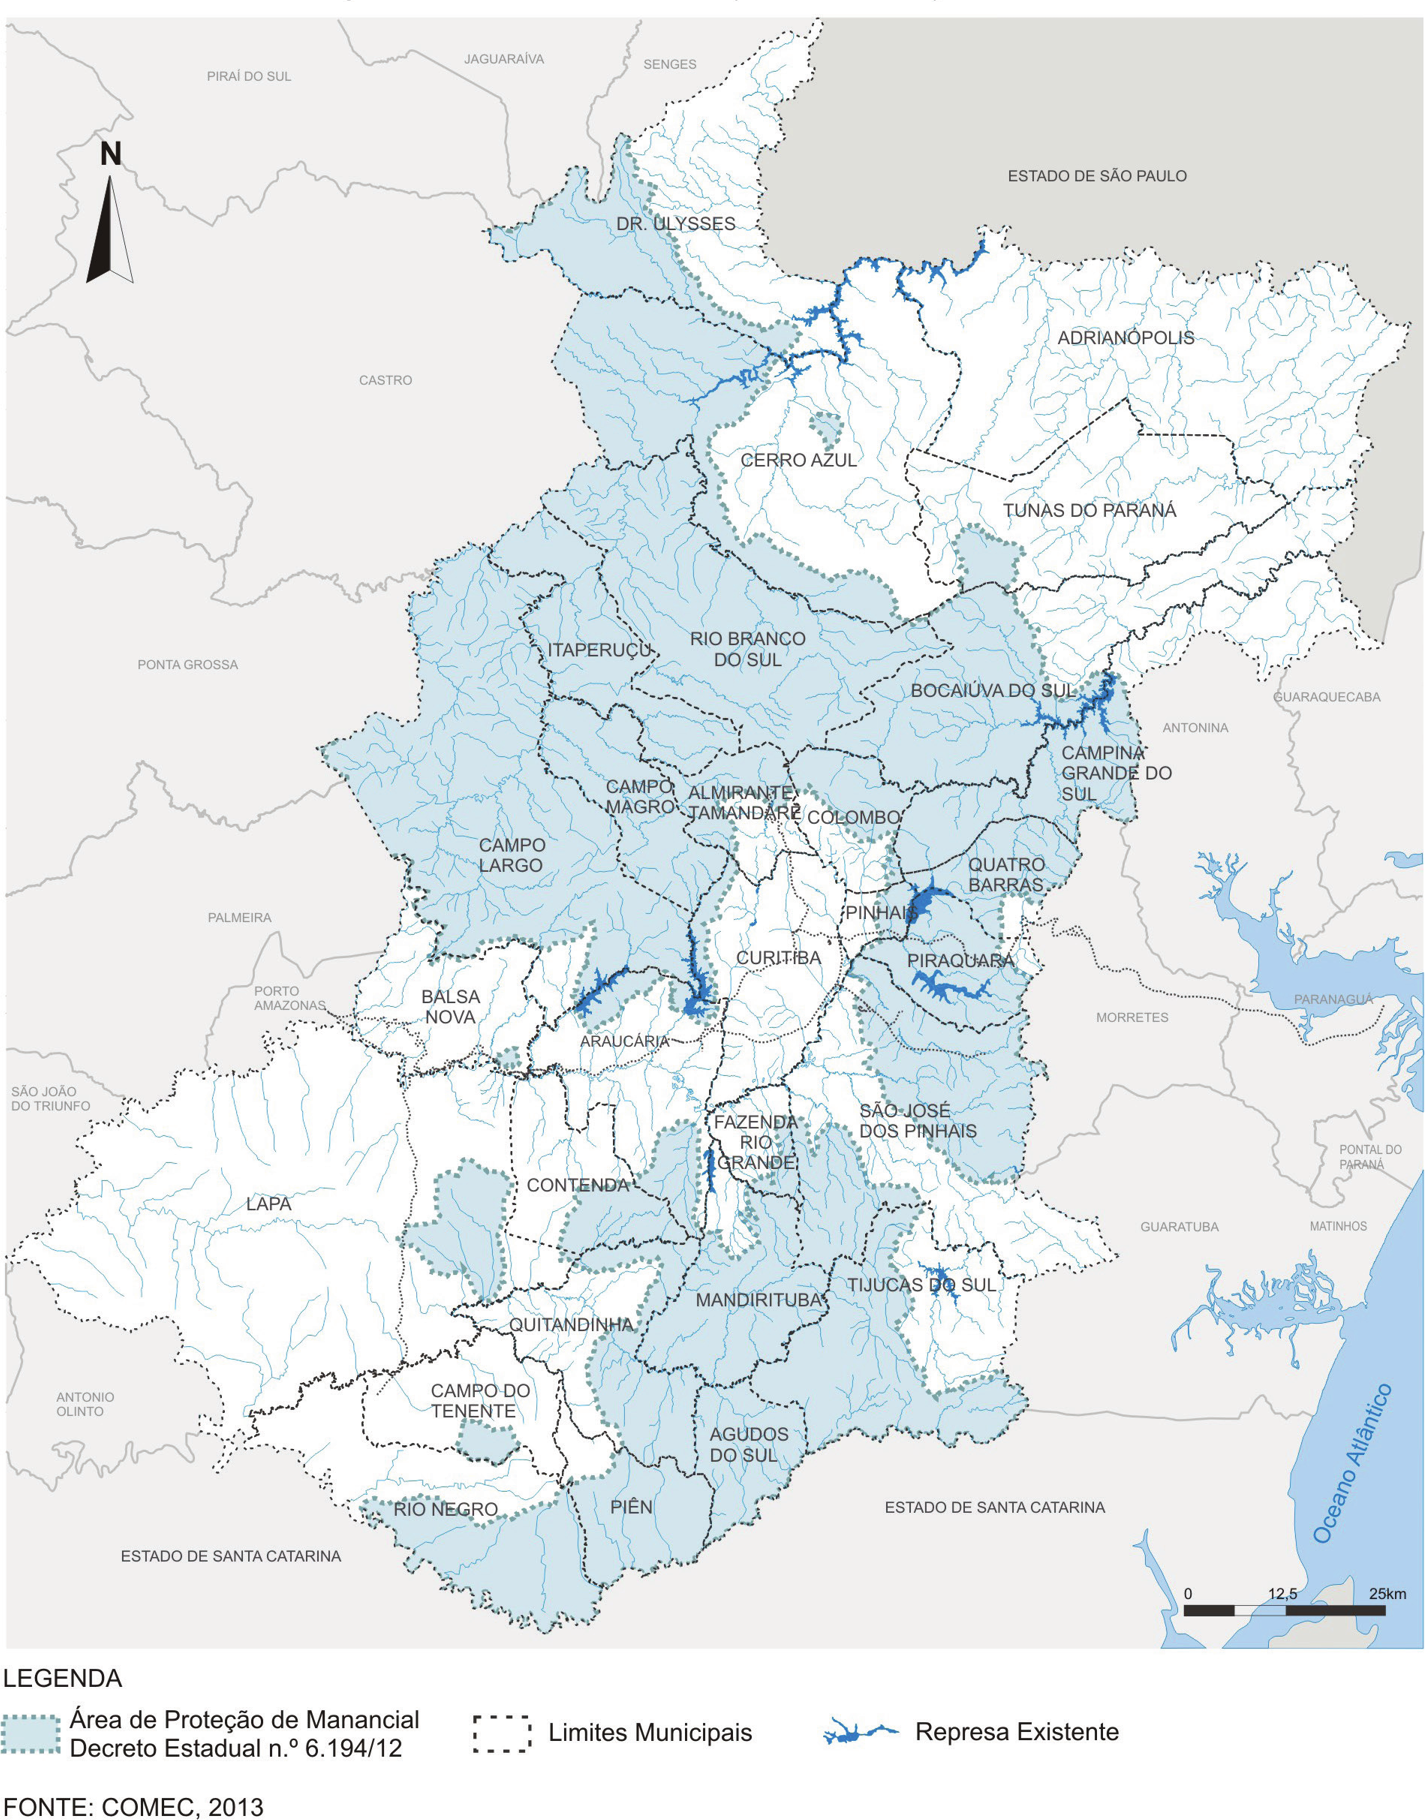
\includegraphics[width=1.0\linewidth]{img/kornin2014a_01}
		\label{fig:kornin2014a_01}
		\legend{Fonte: \citeonline[p. 428]{kornin2014a}}
	\end{figure}

	Segundo \citeonline[p. 5]{andreoli1999a}, a \gls{rmc} está localizada próxima das cabeceiras da Bacia do Iguaçu:
	
	\begin{citacao}
		``A \glsdesc{rmc} - \gls{rmc} está localizada próxima as cabeceiras da Bacia do Iguaçu, na Serra do Mar, que é o seu principal manancial de abastecimento e portanto a disponibilidade de água de boa qualidade representa um dos importantes fatores de limitação do desenvolvimento da região.''
	\end{citacao}

	Como recomenda \citeonline[p. 6]{andreoli1999a},``os mananciais para abastecimento público devem apresentar uma distância das cidades a serem abastecidas viável em termos econômicos sem perder de vista o equilíbrio de sua preservação'', no entanto, a \gls{rmc} viola a recomendação, uma vez que os mananciais são caracterizadas pela proximidade com uma urbanização que se expandiu espontaneamente sobre eles, o que se traduz em: (i) abandono dos investimentos realizados; e (ii) formação de ``verdadeiros cadáveres hídricos, que poluem e envergonham as cidades''.

	\subsection{Saneamento básico}
	% feito pela Mari e incorporado em 15/12/2019
	
	O Saneamento Básico da Região Metropolitana de Curitiba é gerido atualmente pela \gls{sanepar}, e regulada e fiscalizada pela \gls{agepar} desde 28 de dezembro de 2016, após publicação da Lei Complementar 202.
	
	A \gls{sanepar}, que possui sua sede em Curitiba, foi fundada na década de 1960 e hoje em dia atende não apenas a \gls{rmc}, mas 346 dos 399 municípios do Paraná, tornando-a uma das maiores empresas do Estado. É responsável por 54 mil quilômetros de tubulações utilizadas na distribuição de água potável, atendendo 100\% da população urbana dos municípios que serve, e 35 mil quilômetros de rede coletora de esgoto, atendendo 72.5\% da população urbana. Este percentual de atendimento é maior que a média nacional que, segundo o \gls{snis}, é de apenas 59.7\%. 
	
	\begin{citacao}
		``Com base nos dados do Sistema Nacional de Informações sobre Saneamento - \gls{snis} 2014, é válido afirmar que o Estado do Paraná apresenta desafios na gestão de resíduos sólidos similares ao âmbito nacional, como a necessidade de erradicar os lixões. Por outro lado, apresenta alguns dados mais satisfatórios do que a média nacional, como a disposição adequada, que é de 26\% para o Brasil e no Paraná chega a 45\%, com 50\% para o Rio Grande do Sul e 65\% para o Estado de Santa Catarina.'' \cite{anjos2016a}
	\end{citacao}

	Foram confeccionados mapas com percentual de atendimento por município da \gls{rmc}, vide \autoref{fig:saneamentototal}, \autoref{fig:saneamentourbano} e \autoref{fig:saneamentorede}. Vale ressaltar que para os municípios de Adrianópolis, Tunas do Paraná, Rio Branco do Sul, Tijucas do Sul, Piên e Campo do Tenente não foram encontrados dados de atendimento de esgoto em nenhuma fonte de informação oficial (\gls{snis} ou \gls{sanepar}), o que pode indicar uma rede urbana incipiente.
	
	\begin{landscape}
		\begin{figure}
			\centering
			\caption{Atendimento Saneamento Total}
			\label{fig:saneamentototal}
			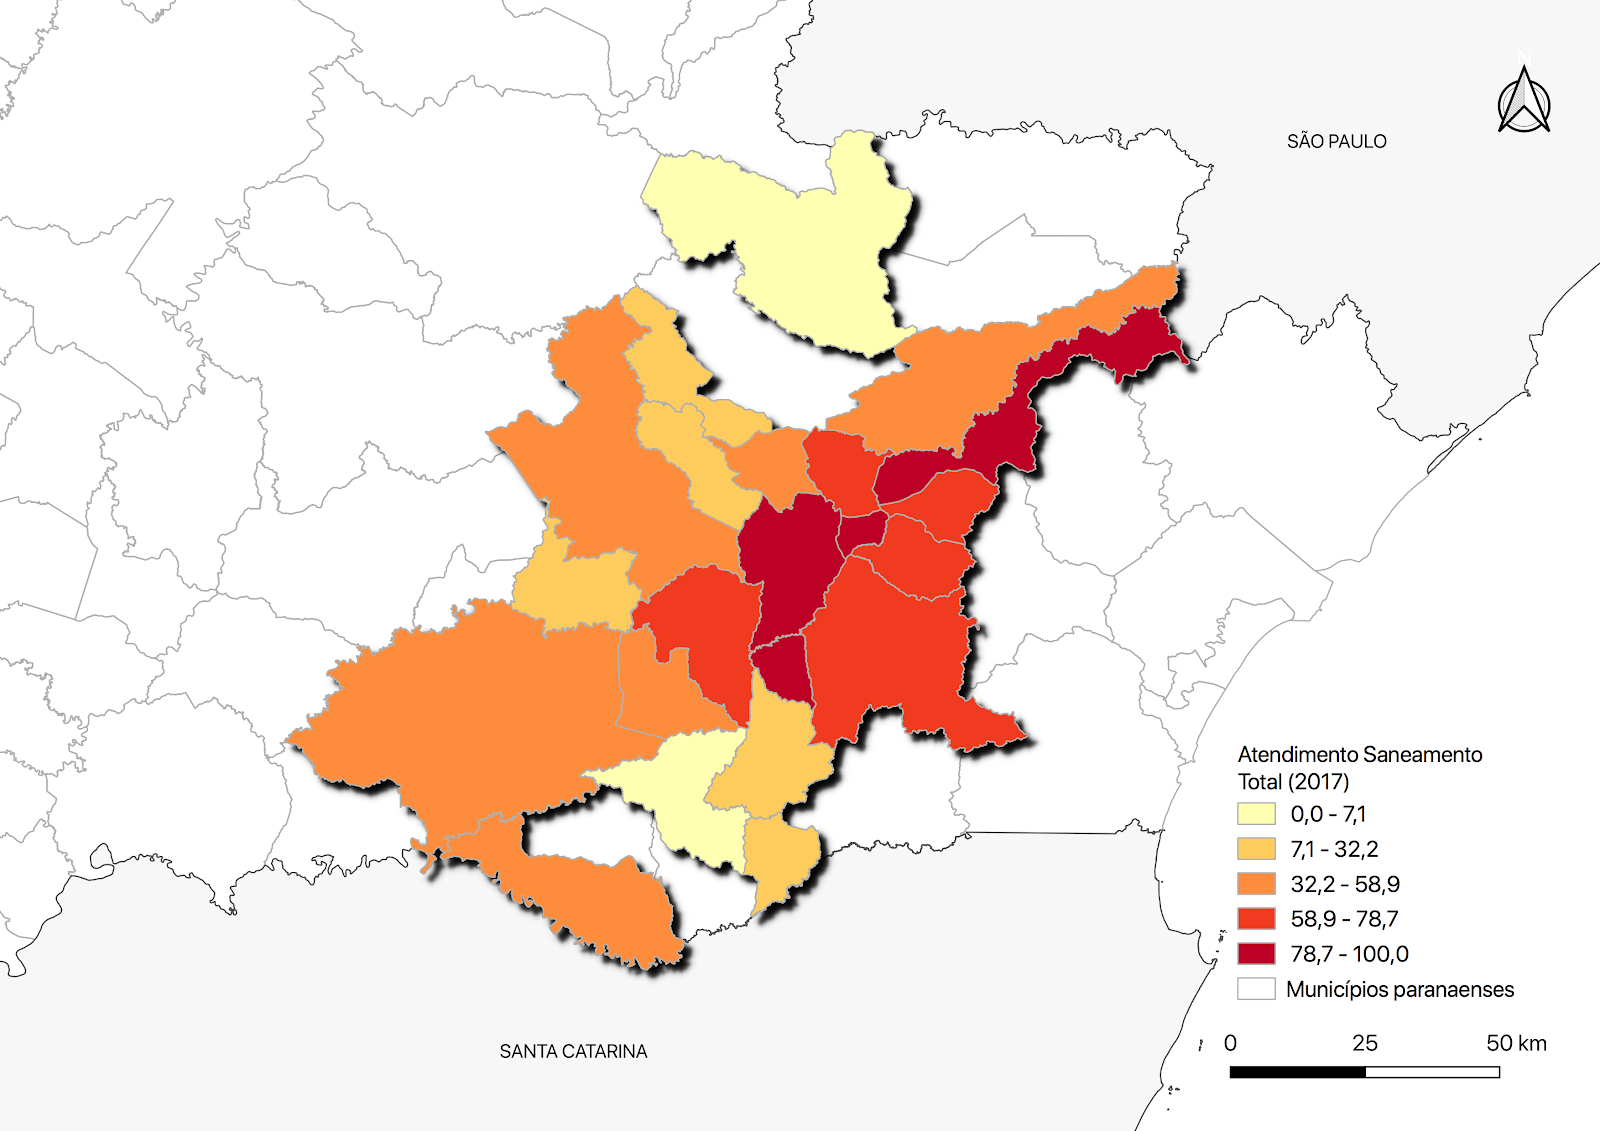
\includegraphics[width=0.80\linewidth]{img/snis_A}
			\legend{Fonte: SNIS, 2017. Elaboração própria}
		\end{figure}
	\end{landscape}
	
	\begin{landscape}
		\begin{figure}
			\centering
			\caption{Atendimento Saneamento Urbano}
			\label{fig:saneamentourbano}
			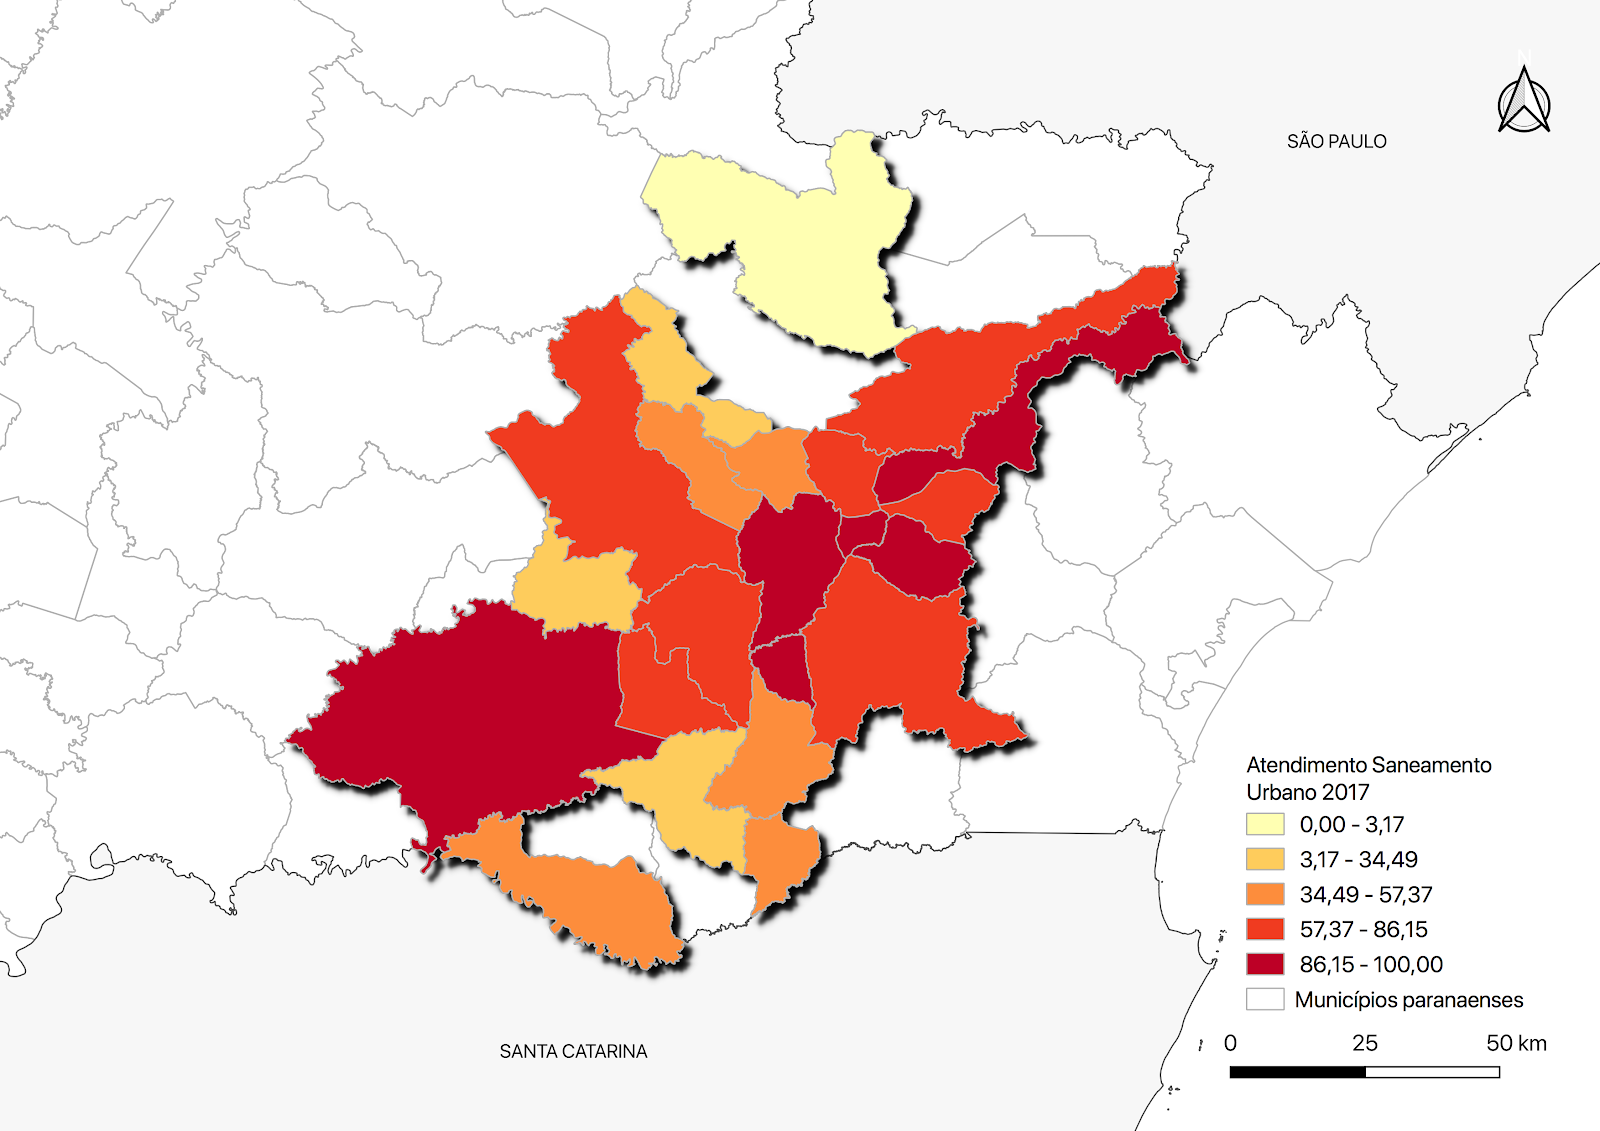
\includegraphics[width=0.80\linewidth]{img/snis_B}
			\legend{Fonte: SNIS, 2017. Elaboração própria}
		\end{figure}
	\end{landscape}

	\begin{landscape}
		\begin{figure}
			\centering
			\caption{Atendimento por rede de distribuição de água}
			\label{fig:saneamentorede}
			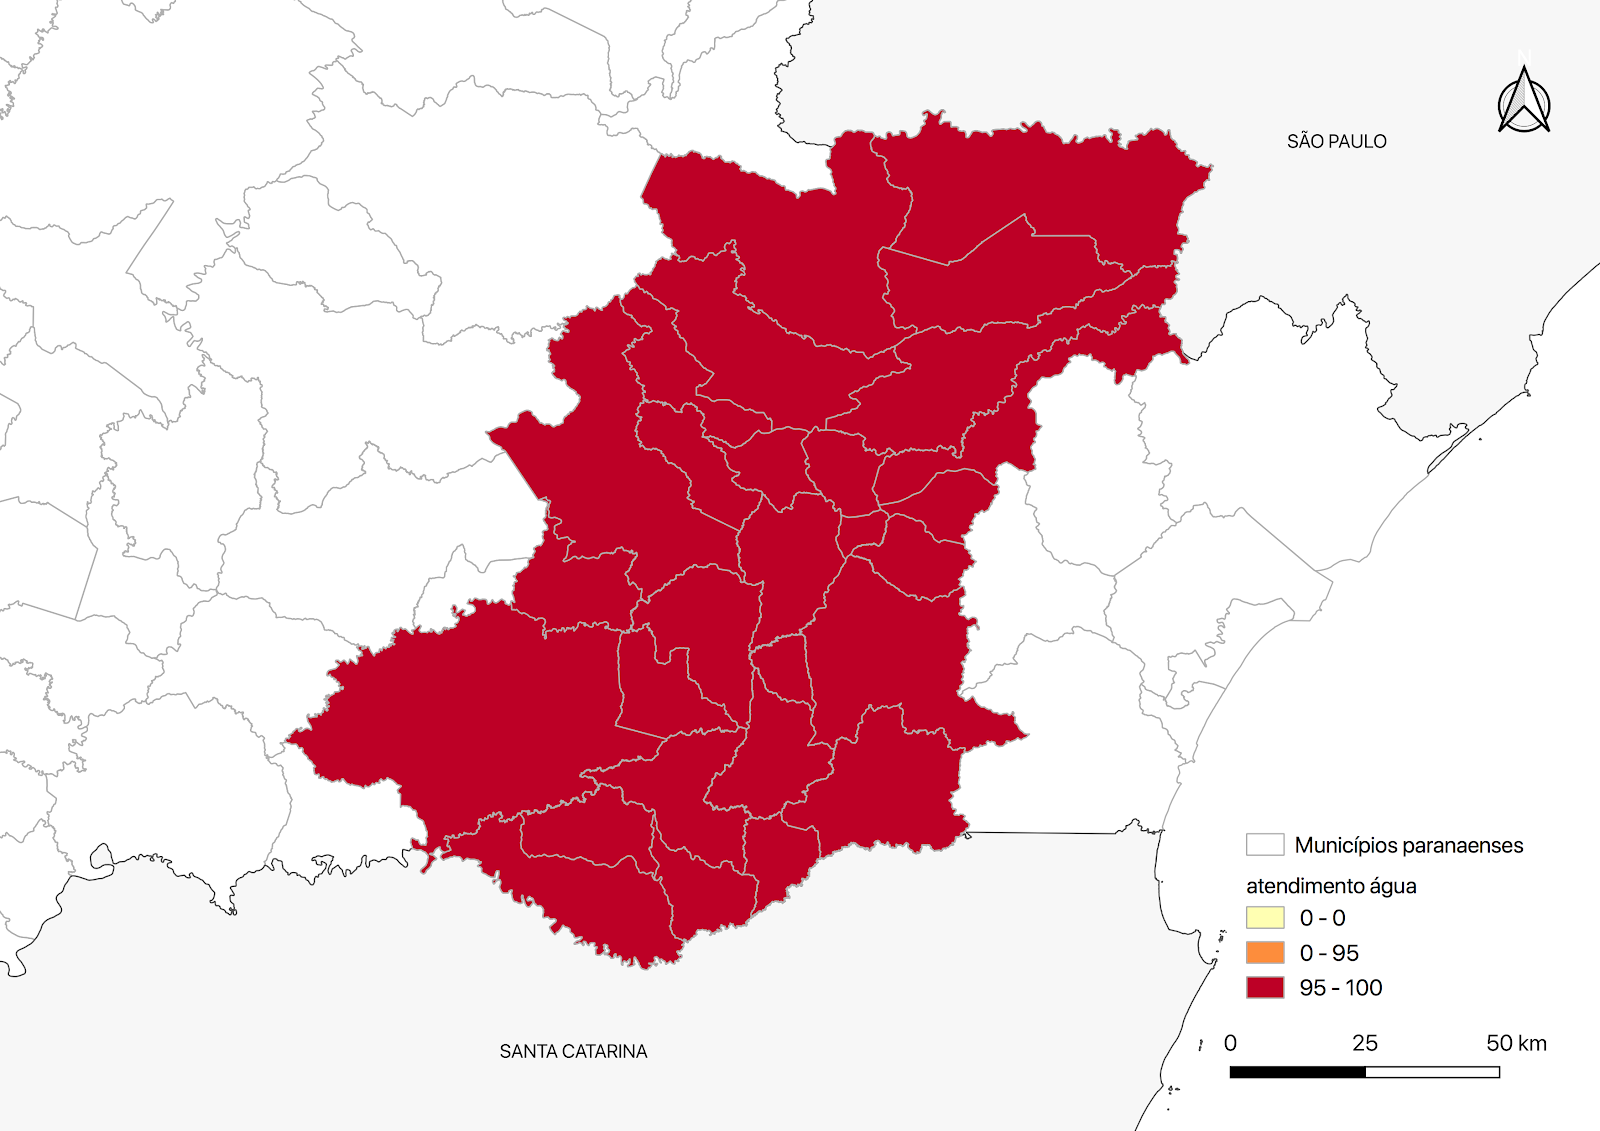
\includegraphics[width=0.80\linewidth]{img/snis_C}
			\legend{Fonte: SNIS, 2017. Elaboração própria}
		\end{figure}
	\end{landscape}

	\subsection{Transportes e sistema viário} \label{sec:transportes}
	% escrito por Caio
	
	A luz do que introduz \citeonline[p. 375]{paese2014a}, o planejamento urbano da capital é especialmente marcante devido à década de 1970 e a implantação de um sistema de transporte coletivo sobre pneus baseados em linhas expressas de ônibus, que atualmente operam com veículos biarticulados em vias segregadas. A inserção das vias segregadas se dá a partir de uma lógica de eixos trinários radiais (centro-bairro/bairro-centro), que contribuíram para estruturar o adensamento construtivo e a verticalização:
	
	\begin{citacao}
		``O planejamento urbano de Curitiba, implantado a partir da década de 1970, possui o sistema de transporte como um de seus pilares. Os eixos trinários, compostos por duas vias rápidas de ligação centro-bairro e bairro-centro, contendo ao centro uma canaleta exclusiva para o ônibus expresso (atualmente transformado em biarticulado), foram os grandes estruturadores da expansão urbana, em razão do que tais eixos foram também definidos como locais preferenciais de verticalização e de expansão linear do centro, induzindo o uso, na parte inferior dos edifícios residenciais, de atividades de comércio e serviços.''
	\end{citacao}

	No âmbito de uma discussão de caráter metropolitano, \citeonline[p. 376]{paese2014a} tratam com a naturalidade à incorporação dos municípios do entorno ao sistema de transporte, cujos eixos originalmente foram concebidos restritos aos limites da capital. A incorporação dá origem à \glsdesc{rit} (\gls{rit}):
	
	\begin{citacao}
		``As linhas que constituem a \gls{rit} são as que podem estabelecer integração físico-tarifária em terminais ou estações com o Sistema de Transporte de Curitiba. É caracterizada por apresentar uma hierarquia de tipos de linhas de ônibus, podendo estar vinculadas a um terminal ou não. As linhas vinculadas a terminais de transporte ou estações--tubos estabelecem uma integração físico-tarifária na qual o passageiro, pagando apenas uma tarifa, pode descer de um ônibus e ingressar em outro que também esteja vinculado ao terminal ou estação-tubo. Os terminais e estações-tubo estão localizados nos municípios integrados, nas vias expressas do sistema de \glsdesc{brt} (\gls{brt}) e em outras importantes vias de Curitiba e municípios mais próximos.'' \cite[p. 376]{paese2014a}
	\end{citacao}
	
	Segundo \citeonline[p. 378]{paese2014a}, além de não atender a uma crescente demanda metropolitana, ``se encontra muito aquém da procura quantitativa e qualitativa, de caráter espaço-temporal, exigida para o deslocamento das pessoas dentro do próprio município de Curitiba''.
	
	Com relação à tecnologia adotada, \citeonline[p. 42]{guia2015a} definem o \gls{brt} como um sistema de transporte público coletivo com elevado desempenho, o que se deve a sua também elevada priorização no sistema de mobilidade e adoção de linhas de ônibus estruturais em sua composição. \citeonline[p. 42]{guia2015a} definem como características do \gls{brt} a circulação de linhas troncais com ônibus circulando em pistas ou faixas exclusivas; possibilidade de ultrapassagem, mesmo que apenas nas áreas de paradas; estações de embarque e desembarque dotadas de sistema de bilhetagem com validação externa aos veículos (pré-embarque), fechadas e em nível; desenho universal de acessibilidade; presença de sistemas para controle operacional e monitoramento; prioridade semafórica; e adoção de paradigma de tronco-alimentação para racionalização do sistema de transporte existente, que atua como alimentador do \gls{brt}.
	
	A caracterização feita por \citeonline[p. 62]{guia2015a} envolve ainda uma série de aspectos gerais e operacionais. O sistema de \glsdesc{brt} da capital surgiu em 1974, atingindo 81 km de extensão ao longo dos anos, resultando em um atendimento de 2,3 milhões de passageiros na \gls{rit}. As paradas (chamadas de estações-tubo, no caso específico de Curitiba) são posicionadas à direita, sem escalonamento e há a presença de serviços expressos e faixas de ultrapassagem nas paradas. Segundo \citeonline[p. 62]{guia2015a}, o município foi pioneiro ao priorizar o transporte público por meio de corredores exclusivos na década de 1970, que se tornaram eixos estruturadores do crescimento urbano:
	
	\begin{citacao}
		Curitiba foi pioneira na priorização do transporte coletivo com a implantação de seu primeiro corredor exclusivo para a circulação dos ônibus em 1974. O sistema possui inovações operacionais que foram incorporadas ao longo do tempo e a tornaram um modelo para cidades brasileiras e estrangeiras (canaletas, serviços expressos e diretos, terminais, estações tubo, tronco-alimentação). Sua concepção é anterior à utilização do termo \gls{brt}. Atualmente, a Rede Integrada de Transportes atende 13 municípios da região metropolitana com ônibus municipais e intermunicipais. A estruturação do sistema de transporte foi cuidadosamente planejada de forma integrada ao planejamento urbano. Os corredores funcionam como eixos estruturantes para o desenvolvimento urbano pois concentram as demandas pelo transporte por meio do aumento da densidade e da diversificação de usos no entorno.	O Eixo Sul, o mais antigo e mais carregado dos seis corredores, transporta 247 mil 	passageiros por dia entre os terminais Rui Barbosa (no centro) e Pinheirinho, sendo 16 mil por sentido no horário de pico. Assim como os demais eixos, começa a apresentar sinais de saturação. \cite[p. 42]{guia2015a}
	\end{citacao}

	A \autoref{fig:brt3d} apresenta uma perspectiva tridimensional de um corredor \gls{brt} com paradas à esquerda (estação em ilha no canteiro central), espaço para ultrapassagem, cobrança externa aos veículos e segregação do tráfego existente nas outras vias. A configuração curitibana é similar, mas adota estações com paradas à direita, ou seja, nas extremidades opostas, conforme podemos observar na \autoref{fig:brtsul}.
	
	\begin{figure}
		\centering
		\caption{Representação de sistema do tipo \glsdesc{brt}}
		\label{fig:brt3d}
		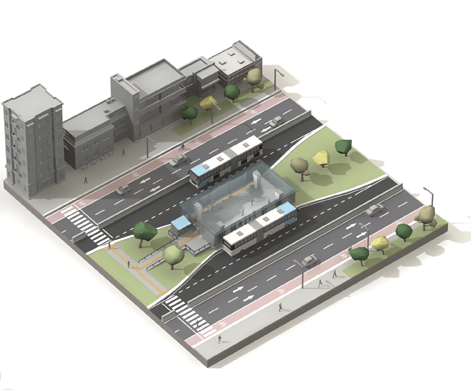
\includegraphics[width=0.65\linewidth]{img/guiatpc2018a_01}
		\legend{Fonte: \citeonline[p. 48]{guiatpc2018a}}
	\end{figure}
	
	\begin{figure}
		\centering
		\caption{Fotografia de estação-tubo e ônibus articulado no \gls{brt} de Curitiba}
		\label{fig:brtsul}
		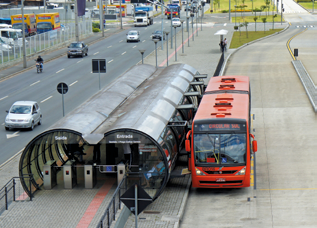
\includegraphics[width=0.65\linewidth]{img/guiatpc2018a_03}
		\legend{Fonte: \citeonline[p. 42]{guiatpc2018a}}
	\end{figure}

	A \autoref{tab:tabonibus} sistematiza as características dos três tipos possíveis de infraestrutura para circulação priorizada de ônibus: faixa exclusiva, corredor central e \gls{brt}.
	
	A \autoref{fig:terminais} espacializa os terminais de ônibus da \gls{rmc} a partir de informações fornecidas pelo \gls{ippuc}.
	
	\begin{landscape}
		\begin{table}
			\centering
			\caption{Quadro-síntese das características para soluções de infraestrutura de priorização com uso de ônibus}
			\label{tab:tabonibus}
			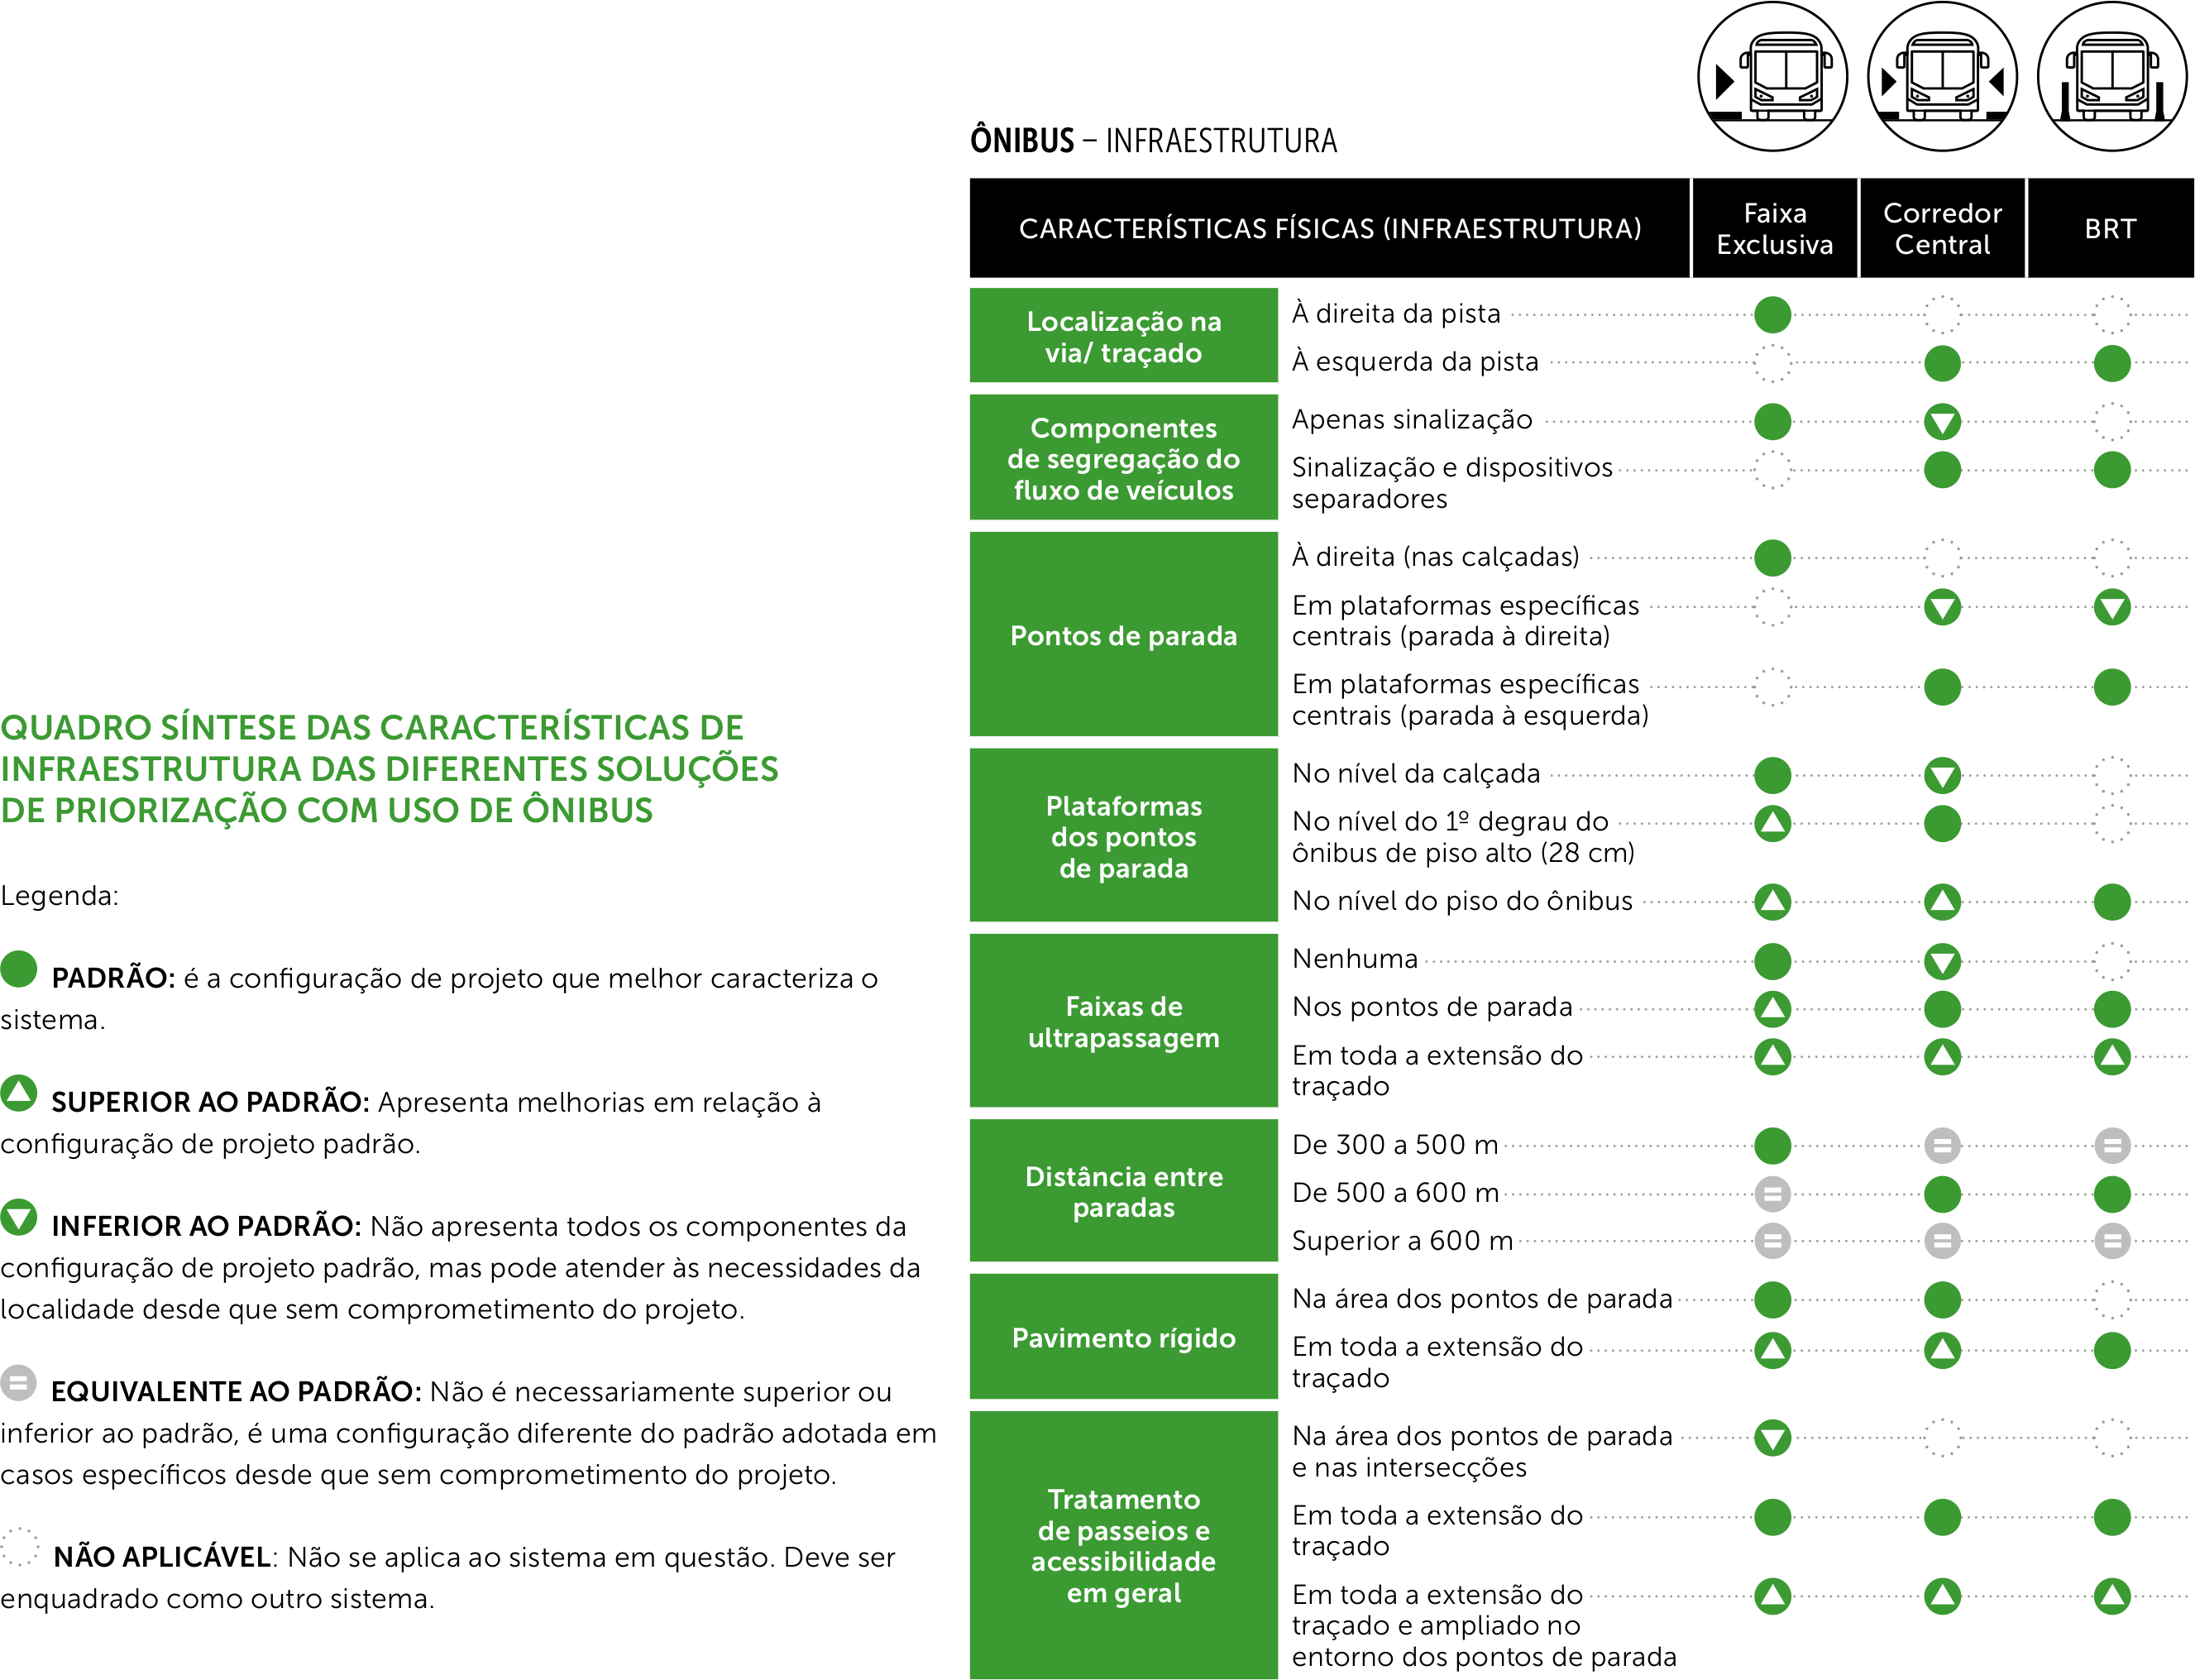
\includegraphics[width=0.75\linewidth]{img/guiatpc2018a_02}
			\legend{Fonte: adaptado de \citeonline[p. 50]{guiatpc2018a}}
		\end{table}
	\end{landscape}

	\begin{landscape}
		\begin{figure}
			\centering
			\caption{Terminais de ônibus da \glsdesc{rmc} por similaridade}
			\label{fig:terminais}
			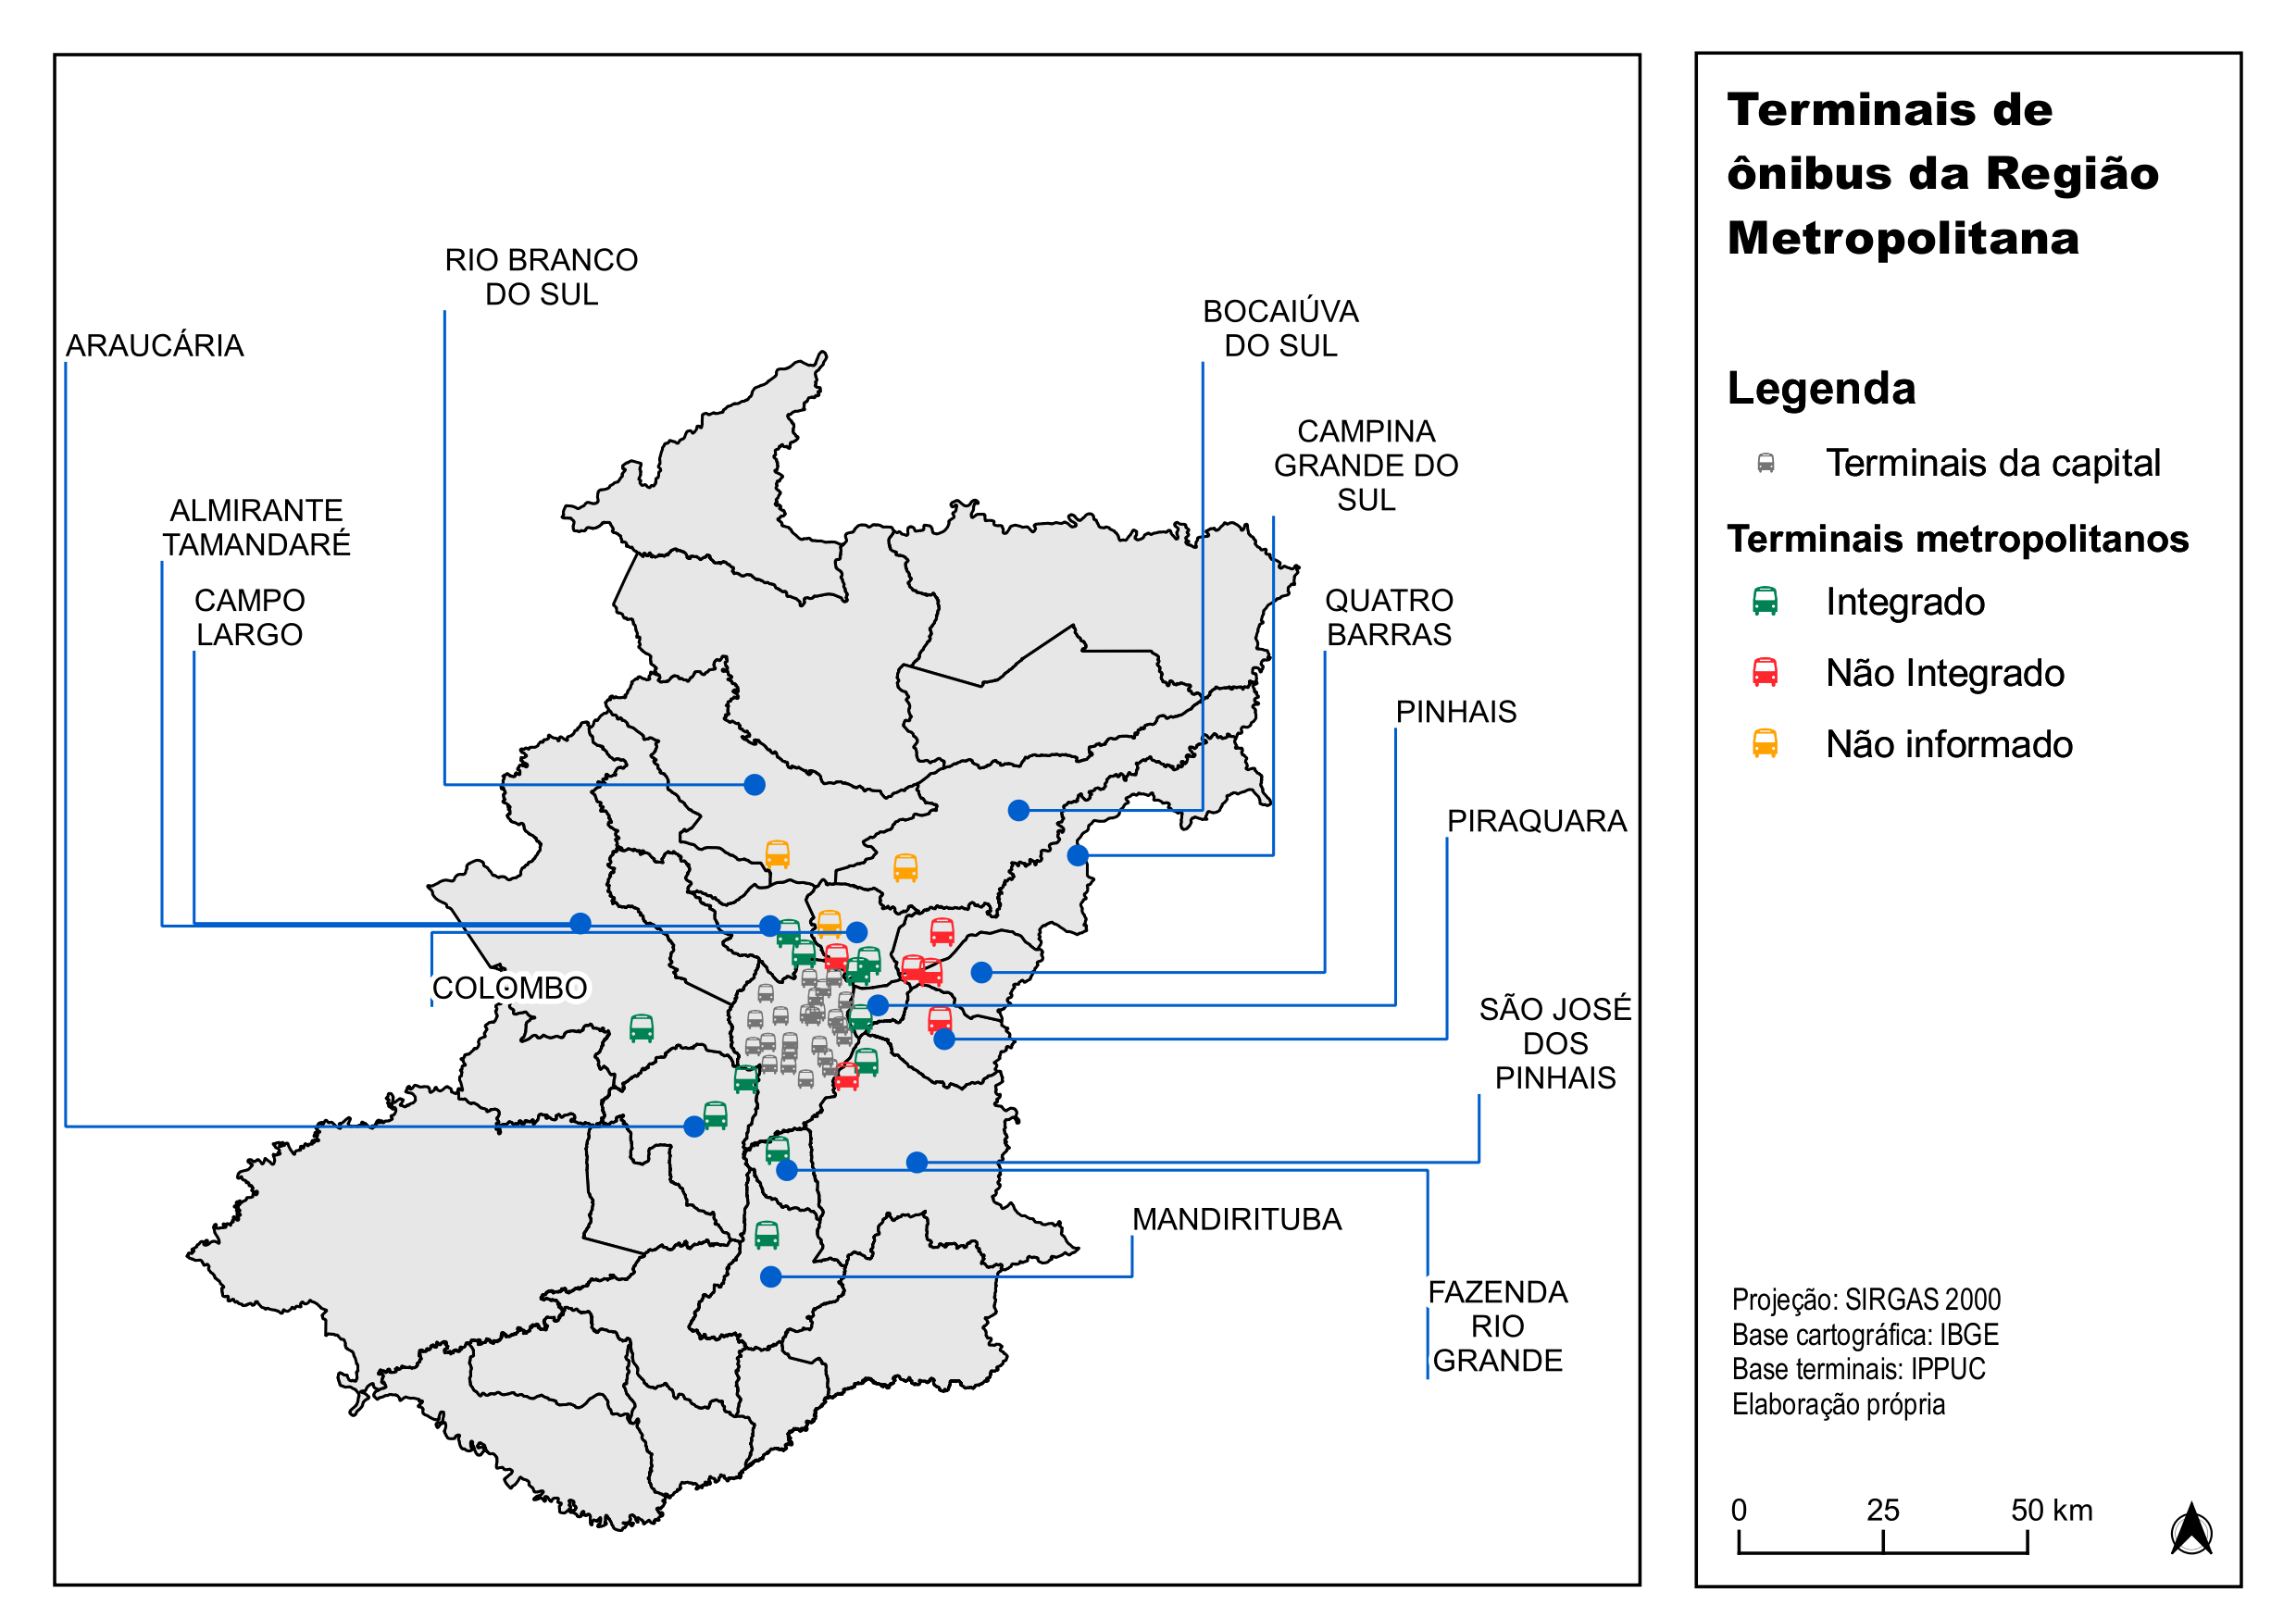
\includegraphics[width=0.85\linewidth]{../gis/produtos/RMC_terminais}
			\legend{Elaboração própria}
		\end{figure}
	\end{landscape}

	Em um conteúdo publicitário da Metrocard, publicado no jornal Gazeta do Povo em 22/11/2019, o ente privado responsável pela interlocução entre estado e o conjunto de 18 empresas associadas que atuam na \gls{rmc}, alguns dados forma fornecidos e organizados na forma de um infográfico (vide \autoref{fig:infograficometrocard}). A Metrocard aponta ainda possuir um \gls{cco} responsável pelo monitoramento de uma frota de 900 ônibus intermunicipais \cite{boreki2019a}.
	
	\begin{figure}
		\centering
		\caption{Dados a respeito do transporte intermunicipal na \glsdesc{rmc}}
		\label{fig:infograficometrocard}
		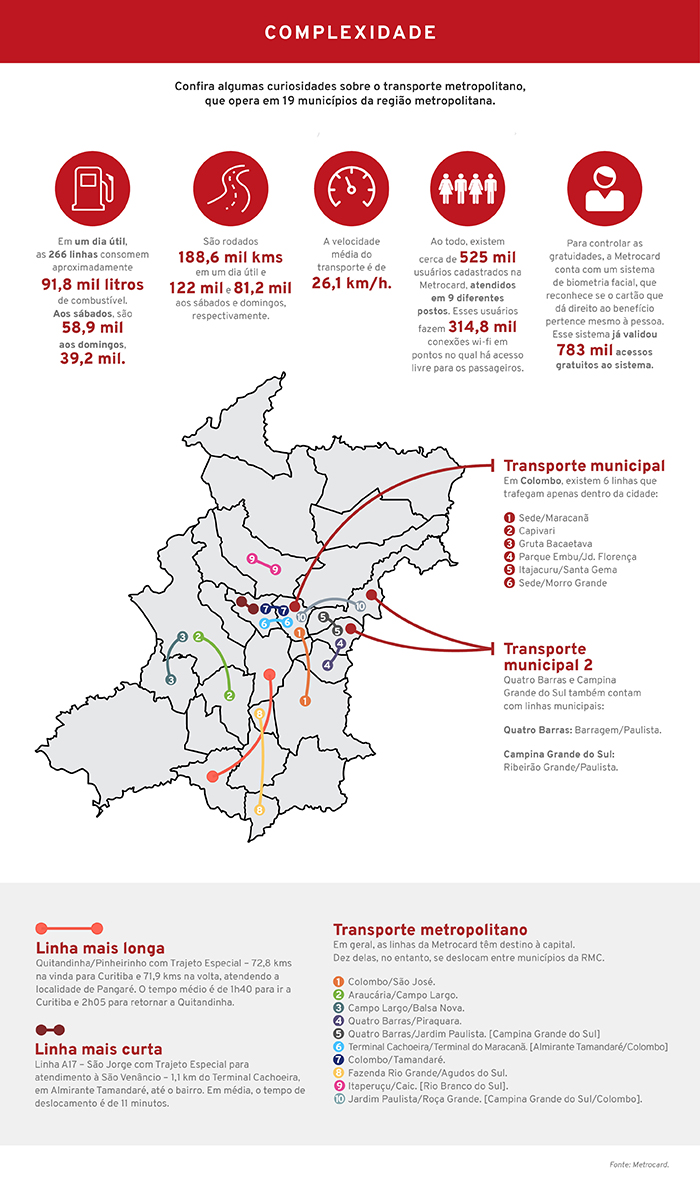
\includegraphics[width=0.80\linewidth]{img/gpovo_A}
		\legend{Fonte: \citeonline{boreki2019a}}
	\end{figure}
		
	Institucionalmente, o arranjo entre o transporte se dá da seguinte maneira:
	
	\begin{citacao}
		``[\dots] a gestão da Rede Integrada de Transporte é realizada mediante instrumento de convênio celebrado entre a COMEC (esfera estadual) e a URBS (esfera municipal de Curitiba), de acordo com o qual o planejamento e o gerenciamento dos serviços de transporte público metropolitano de passageiros na RMC voltaram à responsabilidade da COMEC desde 2012 (CONVÊNIO B, 2012), após 16 anos do primeiro convênio firmado em 1996, quando o órgão delegara as atividades de planejamento e gerenciamento do transporte metropolitano à URBS (CONVÊNIO A, 1996).'' \cite[p. 386]{paese2014a}
	\end{citacao}

	Este arranjo é mencionado no conteúdo publicitário citado anteriormente, com anunciante explicando que não é responsável pela infraestrutura, segurança pública e definição de oferta de lugares (horários dos ônibus):
	
	\begin{citacao}
		``[\dots] as vias por onde trafegam os veículos dependem do poder público (prefeituras e governo estadual, no caso de rodovias estaduais, ou governo federal, no caso de estradas federais), assim como a possibilidade de faixas exclusivas para o transporte coletivo; e a frequência dos veículos é estipulada pela Coordenação da Região Metropolitana (Comec); os terminais são de responsabilidade das administrações municipais ou estaduais; e a segurança pública depende dos órgãos municipais (guarda) e estaduais (Polícia Civil e Militar)'' \cite{boreki2019a}.
	\end{citacao}

	Como pode ser observado na \autoref{fig:paese2014a01}, os maiores fluxos de deslocamentos no grupo de municípios com mais de 10 mil viagens estão nos municípios de Colombo, São José dos Pinhais, Almirante Tamandaré, Pinhais, Fazenda Rio Grande, Araucária e Campo Largo (em ordem decrescente), sendo que pelo ``menos 85\% dos mais do que 10.000 trabalhadores que se deslocam para o trabalho o fazem regularmente'' \cite[p. 384]{paese2014a}.
	
	\begin{figure}
		\centering
		\caption{Fluxo de pessoas dos municípios cujo número total que se desloca para outro município é igual ou maior do que 10.000 - \gls{rmc} - 2010}
		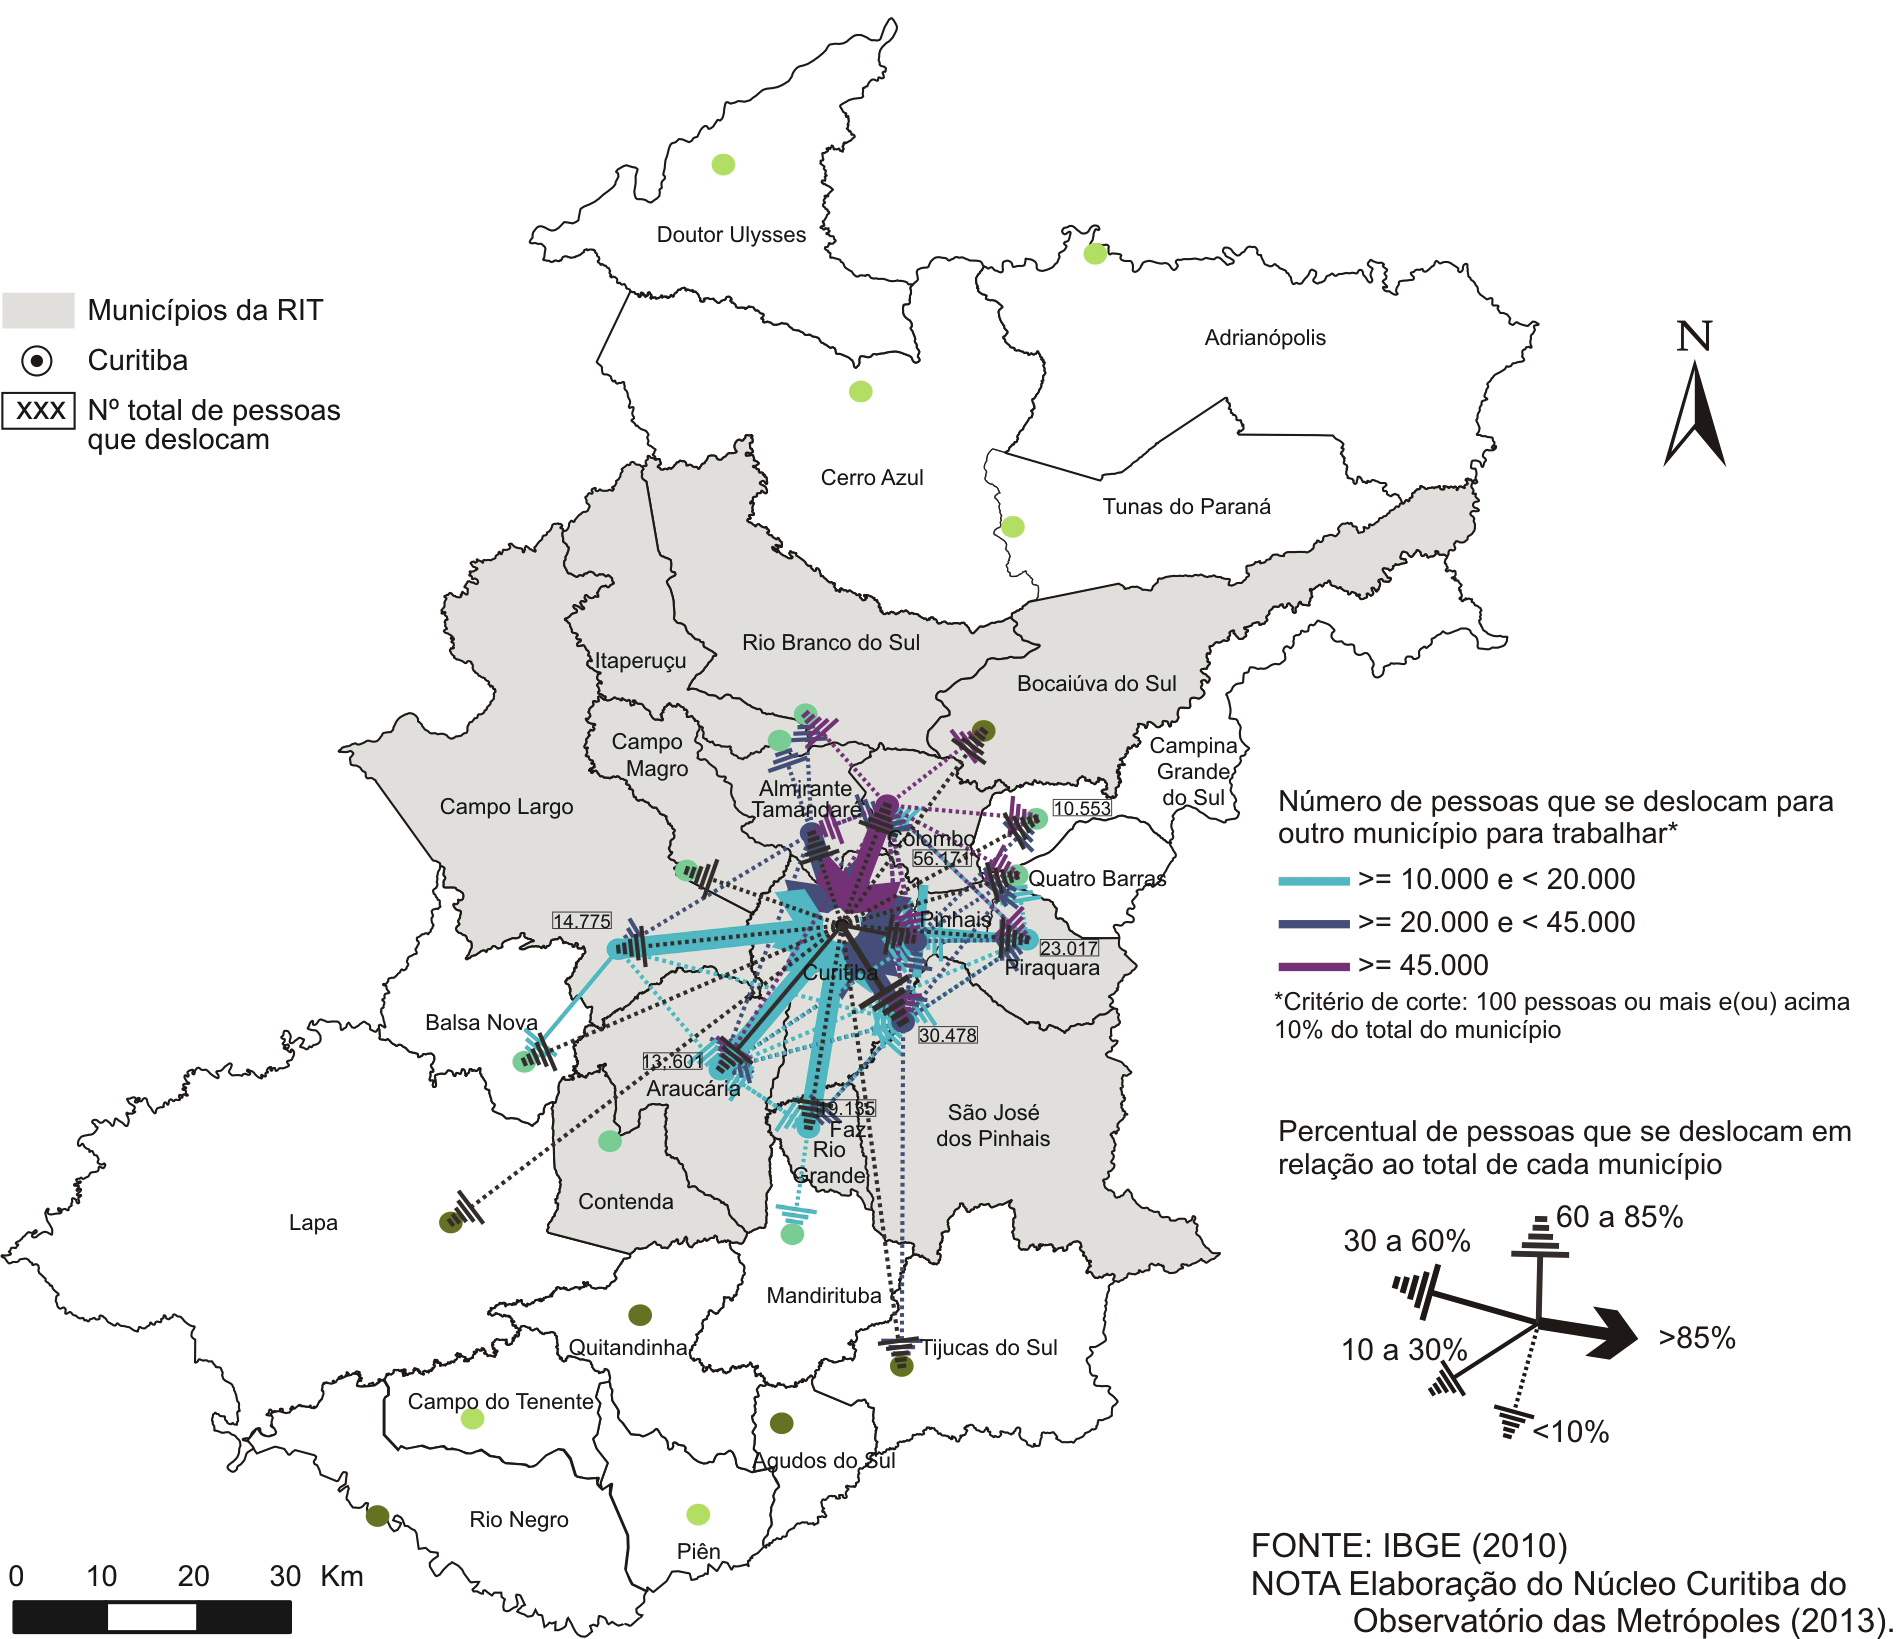
\includegraphics[width=0.7\linewidth]{img/paese2014a_01}
		\label{fig:paese2014a01}
		\legend{Fonte: \citeonline[p. 384]{paese2014a}}
	\end{figure}

	Como pode ser observado na \autoref{fig:paese2014a02}, que representa cartograficamente fluxos pendulares entre municípios com viagens inferiores a 10 mil por motivo de trabalho, existem viagens pendulares entre municípios da \gls{rmc} que não passam por Curitiba, ocorrendo em duas tramas conforme Firkowski, Paese e Nagamine (2014, p. 384-385):(i) “setor norte-leste (Almirante Tamandaré, Itaperuçu, Rio Branco do Sul, Colombo, Bocaiúva do Sul, Campina Grande do Sul e Quatro Barras); e (ii) ``setor leste-sul (Quatro Barras, Pinhais, Piraquara, São José dos Pinhais, Fazenda Rio Grande e Araucária)''.

	\begin{figure}
		\centering
		\caption{Fluxo de pessoas dos municípios cujo número total que se desloca para outro município é menor do que 10.000 - \gls{rmc} - 2010}
		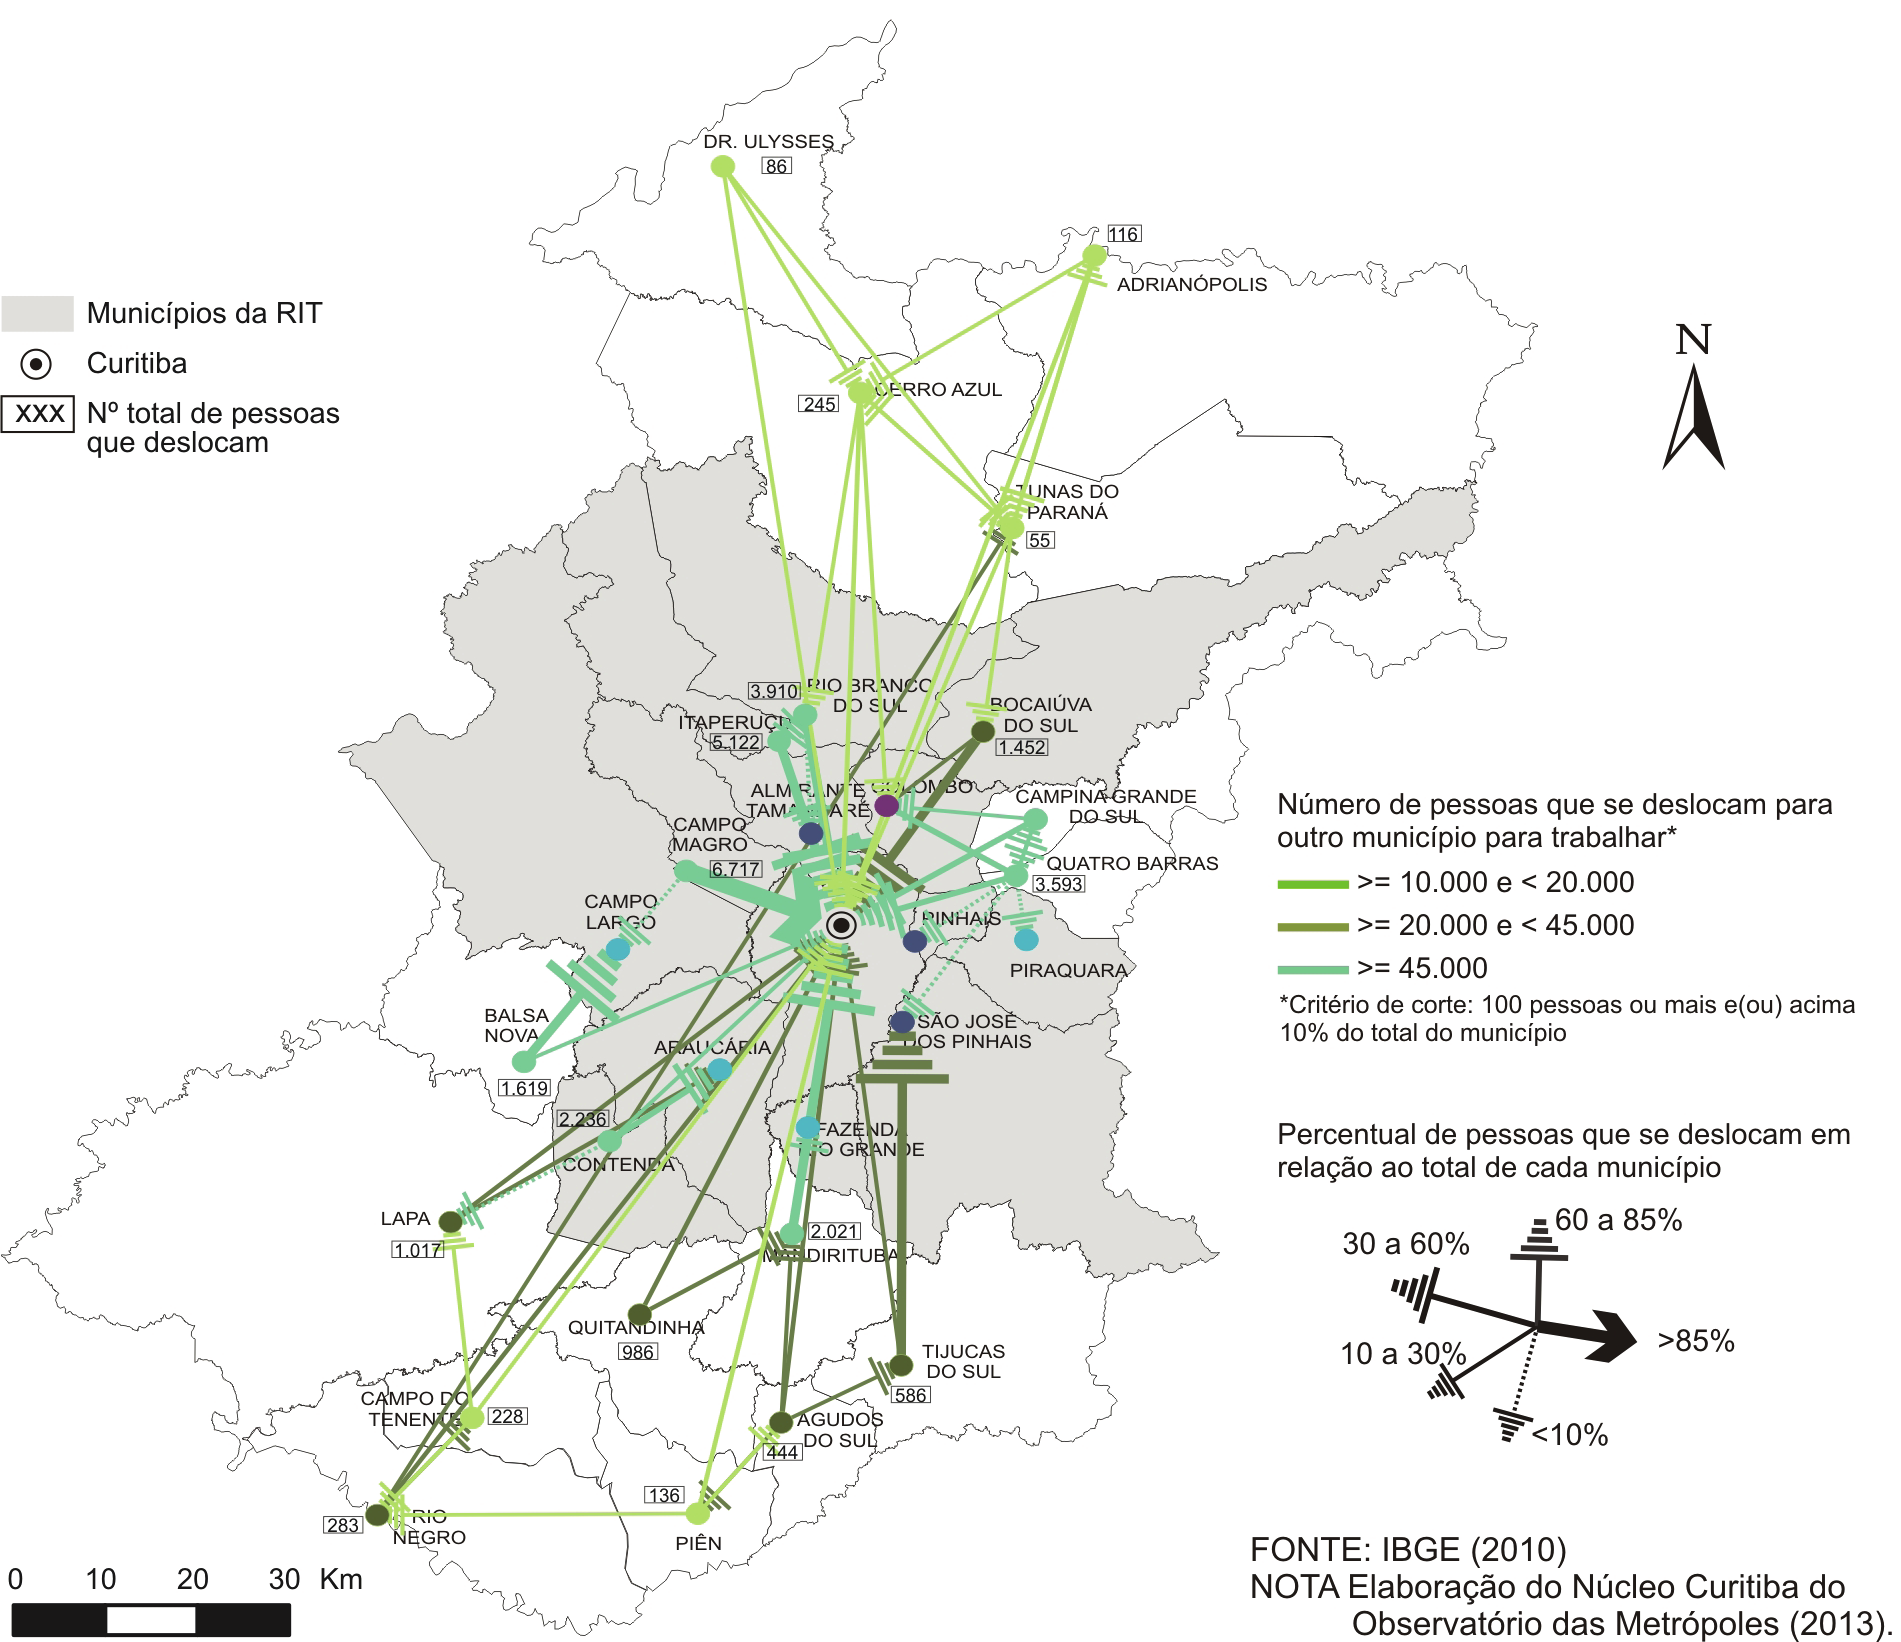
\includegraphics[width=0.7\linewidth]{img/paese2014a_02}
		\label{fig:paese2014a02}
		\legend{Fonte: \citeonline[p. 385]{paese2014a}}
	\end{figure}
	
	\subsection{Habitação}
	% TODO - ajustar trechos abaixos quando resolver plágio
	
	A política habitacional na \glsdesc{rmc} surge com a criação da Companhia de Habitação Popular de Curitiba, em maio de 1965, que objetivava atuar em conjunto com o Sistema Financeiro de Habitação, então recém-criado \cite[p. 81]{colin2009a}, no entanto, este sistema, que se voltava à produção de moradia para classes médias e altas financiadas privadamente e a partir de recursos do \gls{fgts} para moradias populares, nos dois casos sob tutela do \gls{bndes}, desidratou a partir da segunda metade década de 1980, sendo o \gls{bnh} extinto em 1986. Com a chegada da Caixa Econômica Federal, a lógica adotada foi de captação e não de fomento, ``caracterizando a descentralização ocorrida por
	uma absoluta ausência da política nacional, aliada à pressão popular'' \cite[p. 82]{colin2009a}.
	
	A escassez de recursos e políticas públicas habitacionais de âmbito nacional forçaram estados e municípios a buscarem saídas de gerenciamento próprias, afetadas pela escassez de recursos e ausência de cultura de investimento nas escalas local e regional por estes dois atores \cite[p. 82]{colin2009a}. Diante do contexto de fragilização da política habitacional, é oportuno citar \citeonline{castro2005a}:
	
	\begin{citacao}
		``Nos anos 80, uma forte crise econômica no Brasil faz com que o poder público seja pressionado a responder as necessidades básicas sociais, ampliando as áreas destinadas à habitação popular. Em Curitiba, ocorreu no final desta década, a ocupação de um dos últimos grandes vazios urbanos oficiais, chamado Bairro Novo. [\dots]'' \cite[p. 54]{castro2005a}
	\end{citacao}

	Para \citeonline[p. 82]{colin2009a} o desmonte do Sistema Nacional de Habitação culminou num ``processo contínuo de desresponsabilização do Estado pela transferência de suas atribuições à iniciativa privada''.
	
	Ainda que datado, o relato do \gls{mnlm} apontava cerca de 200 ocupações na década passada: ``só em Curitiba, que se diz `Capital Social', existem mais de 200 áreas ocupadas irregularmente, sendo que um grande número destas estão com pedido de reintegração de posse'' \cite[p. 127]{hilma2009a}, número este que se aproxima daquele apontado por \citeonline[p. 84]{colin2009a}, que estimaram 262 áreas ocupadas, afetando um contingente populacional de 250 mil pessoas submetidas a condições sub-humanas:
	
	\begin{citacao}
		No caso de Curitiba, a ausência de uma política específica, integrada com as demais políticas sociais, tem gerado um alto número de áreas de ocupação, correspondendo atualmente a 262 áreas, com aproximadamente 250 mil pessoas vivendo em condições sub-humanas.
	\end{citacao}
	
	% TODO - tem plágio
	% fonte cadastrada como vaccari2018a no fontes.bib
	% plágio - p. 23 - https://acervodigital.ufpr.br/handle/1884/57167
	Utilizando-se do novo modelo de planejamento e gestão metropolitanos no estado do Paraná, exigência advinda da aprovação em 2015 da Lei Federal 13.089 - Estatuto da Metrópole -, é preciso compreender como os PDIs influenciam para a discussão da redefinição e gestão das FPICs na metrópole de Curitiba. Segundo o artigo que recebe o mesmo título deste subcapítulo, da autora Lorreini Vaccari, de acordo com os PDIs, verificou-se a interpretação da moradia como demanda metropolitana setorial, limitada à produção de habitação e lotes para a população de baixa renda, cabendo ao órgão metropolitano um papel auxiliar, de suporte à COPAHAR e à COHAB-CT. Observou-se também a não utilização de ferramentas e ações específicas e articuladas aos instrumentos de uso do solo para o tratamento da moradia na metrópole, confirmando-se que a questão não possui centralidade no planejamento metropolitano e nem é interpretada como FPIC geradora e articuladora das demais demandas urbano-metropolitanas. Segundo a autora, tal visão setorial é também recorrente e estruturante dos discursos, técnico e político vigentes. O não reconhecimento da moradia como FPIC contribui para o enfraquecimento do planejamento urbano na metrópole de Curitiba, bem como do próprio órgão metropolitano, que ao interpretar a moradia setorialmente e não articulada às demandas metropolitanas, limita sua ação e o potencial de seus efeitos sociais e territoriais, reproduzindo e contribuindo com o aprofundamento das desigualdades socioespaciais.
	
	A partir dessa perspectiva, e compreendendo a metrópole contemporânea como um produto do processo de metropolização do espaço, definido como um momento de maior complexidade da urbanização, é preciso que se articulem esses territórios urbanizados, que como demonstrado em seu desenvolvimento histórico, foi caracterizado pela fragmentação e aprofundamento das desigualdades socioespaciais e pela ampliação da polarização social, bem como pela complexificação das relações socioeconômicas e sociopolíticas.
	
	Historicamente, os planos e programas de investimento implementados pela COMEC não tiveram vigor suficiente para alterar a realidade do processo de produção do espaço metropolitano a partir da lógica de periferização e precarização da moradia que, capturada pela lógica de cidade mercadoria, produz uma metrópole cada vez mais marcada pela segregação socioespacial, permitindo evidenciar a moradia como questão fundamental e FPIC central para o planejamento metropolitano. 
	
	A questão da moradia também revela o modelo a partir do qual a metropolização brasileira tem se consolidado, com profundas desigualdades socioespaciais. Estudos realizados pela Fundação João Pinheiro em parceria com o Ministério das Cidades, apresentaram para o Censo de 2010, uma carência de 6 milhões e 940 mil unidades, com 85\% desse total localizado em áreas urbanas e déficit habitacional urbano relativo às regiões metropolitanas estimado em 3 milhões e 299 mil unidades, ou seja, aproximadamente 50\% do déficit habitacional do país (FJP, 2013).
	
	De acordo com a pesquisa de Vaccari, a constatação de que a moradia não foi arrolada legalmente como FPIC na RMC e não constitui elemento orientador da atuação da Coordenação da Região Metropolitana de Curitiba (COMEC), desde a sua criação, associada à atuação setorial e desvinculada de uma política pública de moradia metropolitana do Governo do Estado do Paraná e da Prefeitura Municipal de Curitiba no tratamento da problemática da moradia na metrópole, permitiram formular o problema de pesquisa, que parte basicamente do fato de que, se a moradia pode ser entendida como geradora das demais demandas da população urbano-metropolitana e, portanto, transversal e articuladora das demais FPICs, o não reconhecimento da moradia como questão central e crucial ao planejamento territorial, reforça o tratamento setorial das políticas urbanas, aprofundando as desigualdades socioespaciais. Assim, o não reconhecimento da moradia como FPIC pela entidade metropolitana contribui para o enfraquecimento do planejamento urbano como tributário do acesso à metrópole em Curitiba, bem como da própria entidade metropolitana, que deveria ser a instância mediadora e articuladora dos entes federativos para a gestão dos interesses comuns metropolitanos.
	
	\subsection{Resíduos sólidos}
	% eu acho que foi feito por um dos Gustavos
	
	A \gls{rmc} possui o Consórcio Intermunicipal para Gestão dos Resíduos Sólidos Urbanos, que é composto pelos municípios de: Almirante Tamandaré; Araucária; Balsa Nova; Campina Grande do Sul; Campo Largo; Campo Magro; Colombo; Contenda; Curitiba; Fazenda Rio Grande; Mandirituba; Pinhais; Quatro Barras; Quitandinha, e São José dos Pinhais. O prazo de duração do consórcio é indeterminado.
	
	\section{Gestão}
	
	\subsection{COMEC}
	
	% TODO - incorporar
	\begin{citacao}
		``Apesar da constituição da \glsdesc{comec} (\gls{comec}), como órgão responsável pela `articulação e coordenação das ações de interesse comum no espaço regional', Curitiba se caracteriza como a principal força decisória da região devido ao destacado poder político e econômico da metrópole ante os demais municípios da Região Metropolitana. Isso repercute na ocupação privilegiada de vários espaços eletivos de representação como a Associação dos	Municípios da Região Metropolitana (Assomec) e o Fórum dos Gestores Municipais
		de Assistência Social (Fogemas), ficando os outros municípios com baixo poder de pressão, de pactuação e negociação política e, por conseguinte, com dificuldade	em defender seus interesses.'' \cite[p. 84]{colin2009a}
	\end{citacao}
	
	\subsection{IPARDES}
	
	\subsection{IPPUC}
	
	\section{Orçamento e financiamento}
		
	\begin{figure}
		\centering
		\caption{Receita Municipal per capita segundo o tamanho dos municípios da \gls{rmc}}
		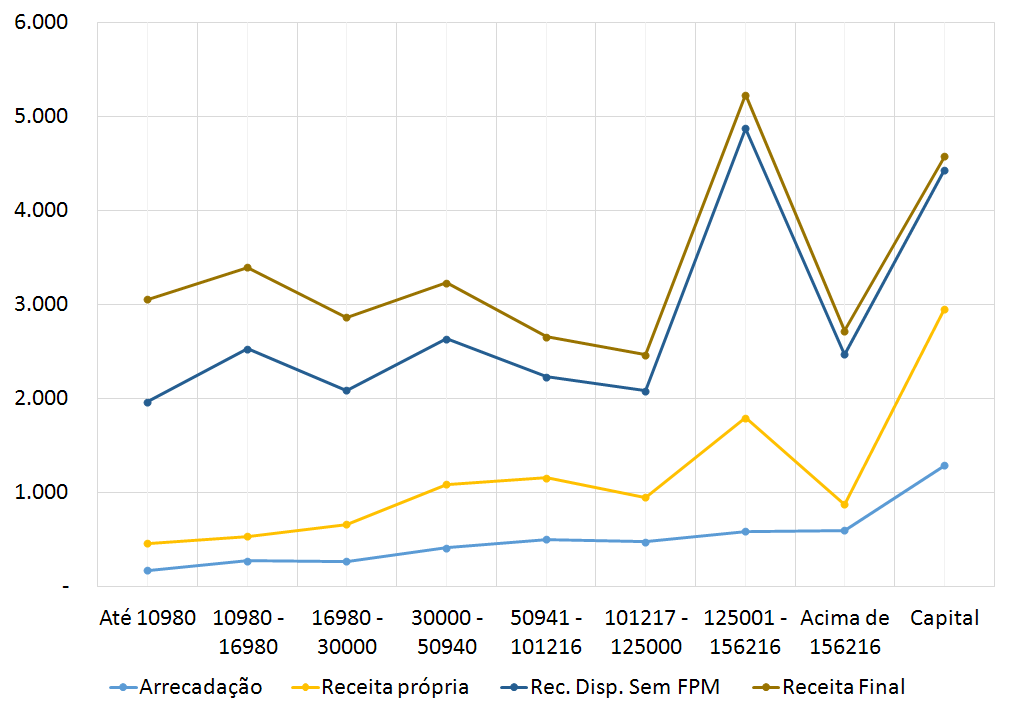
\includegraphics[width=1.0\linewidth]{img/orcamento_A}
		\label{fig:orcamento}
		\legend{Elaboração própria}
	\end{figure}
	
	\section{Governança}
	
	\chapter{Prognóstico} \label{sec:prognostico}
	
	\section{Cinturão verde}
	% Introdução feita pela Mari
	
	Segundo \citeonline[p. 14]{khatib2018a}, o conceito de cinturão verde aparece, não apenas no Brasil, como uma ``configuração social e econômica tipicamente rural, como uma área [\dots] voltada para o abastecimento da metrópole''. Menções a este tipo de arranjo existem desde a antiguidade. De acordo com artigo publicado no site URBAN HUB, especializado em urbanização, no século VII um decreto em Medina ``proibiu a remoção de árvores em uma faixa de quase 20 quilômetros ao redor da cidade'' \cite{urbanhub2017a}.
	
	Portanto, podemos dizer que a esfera ambiental em um arranjo urbano engloba e contempla também a esfera social, e não apenas aquilo que é natural, como comumente associado. De acordo com
	\citeonline[p. 2003]{sposito2003a} ``[\dots] o ambiental não se restringe ao conjunto de dinâmicas e processos naturais, mas das relações entre estes e as dinâmicas e processos sociais''.
	
	Por conseguinte, torna-se necessário que o planejamento do espaço urbano considere o papel dos elementos naturais, juntamente com sua vocação, durante seu desenvolvimento.
	
	Nesta seção, buscaremos apresentar alguns casos que serviram como fontes de informação e debate para nossa proposta de rearranjo da \glsdesc{rmc}.
	
	\textbf{Observação:} para antecedentes sobre a dinâmica de ocupação da \glsdesc{rmc}, sobretudo em relação ao tipo de planejamento conduzido durante a década de 1970, que visava estabelecer um modelo de desenvolvimento territorial equilibrado, consultar a \autoref{sec:ocup1970}.
	
	\subsection{Portland como estudo de caso}
	% feito por Caio com base em trabalho anterior na disciplina teórica
	
	Conforme \citeonline[p. 324]{wheeler2003a}, o desenho regional de Portland inicialmente era relativamente simples. Os esforços inicialmente estavam centrados na \gls{ugb}, que foi aprovada em 1979. Nos anos seguintes, surgiu a consciência de que eram necessários medidas adicionais para criar bairros compactos e vívidos dentro dos limites da \gls{ugb}, consequentemente, em 1997 o Metro Council finaliza seu plano Region 2040, estabelecendo um conjunto de diretrizes para regular a forma urbana na direção desejada --- o plano era bastante ambicioso no olhar para os próximos 50 anos.
	
	Os planos funcionais da Metro exigiam dos governos locais que aumentassem as densidades residenciais, aumentassem o número de conexões viárias por milha, orientassem que o desenvolvimento se concentrasse ao redor do transporte público e estabelece uma rede de áreas verdes. O Estado do Oregon teve papel-chave na promoção destas estratégias a partir da \gls{dlcd} e \gls{odot}.
	
	\citeonline[p. 60]{noronha2015a} se refere à \gls{ugb} como “perímetro de crescimento inteligente”. A \autoref{fig:ugbjun} a seguir representa os limites da \gls{ugb}.
	
	\begin{figure}
		\centering
		\caption{\glsdesc{ugb} de Portland}
		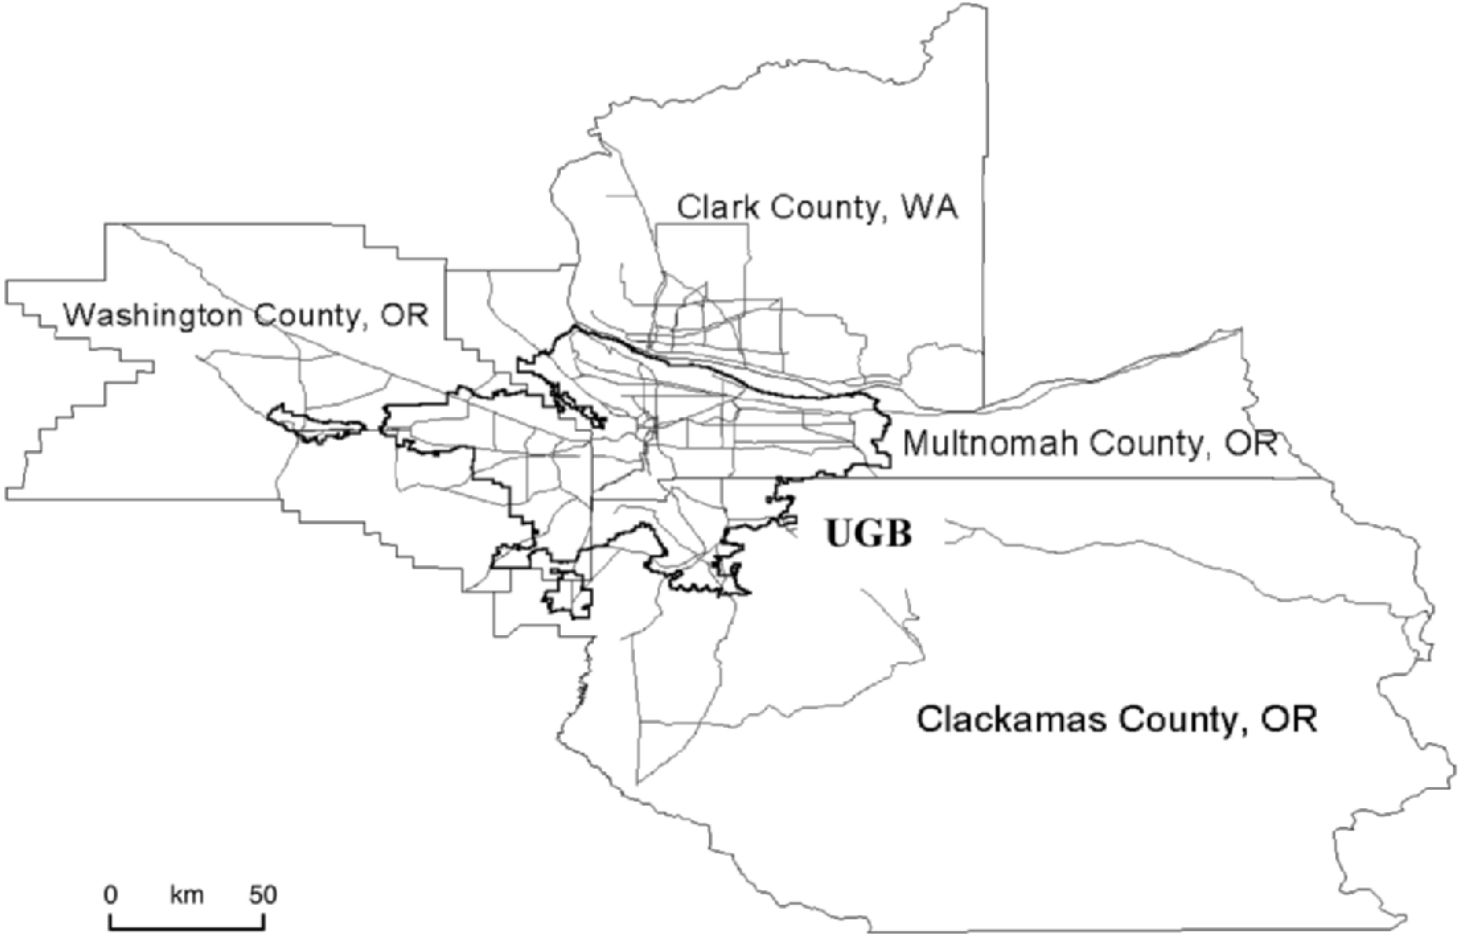
\includegraphics[width=0.9\linewidth]{img/jun2004a_01}
		\label{fig:ugbjun}
		\legend{Fonte: \citeonline[p. 1335]{jun2004a}}
	\end{figure}
	
	O plano previa uma série de desenhos-tipo, conforme \cite[p. 10--11, tradução e grifo nossos]{metro2000a}:
	
	\begin{itemize}
		\item Central city (cidade central);
		\item Regional centers (centros regionais);
		\item Town centers (centros de vilas);
		\item Main streets (avenidas principais);
		\item Corridors (corredores);
		\item Station communities (comunidades das estações);
		\item Neighborhoods (bairros);
		\item \textbf{Neighboring cities/green corridors (cidades vizinhas/corredores verdes)};
		\item \textbf{Rural reserves/open spaces (reservas rurais/espaços abertos)};
		\item Industrial areas and freight terminals (áreas industriais e terminais de carga);
	\end{itemize}
	
	Assim como Curitiba, o plano adotava conceitos de \gls{tod}; no caso de Portland, com eixos de transporte orientando planos de investimentos. A \autoref{fig:todtrimet} exemplifica as duas situações.
	
	\begin{figure}
		\centering
		\caption{Conceitos de \gls{tod} sendo aplicados em Portland}
		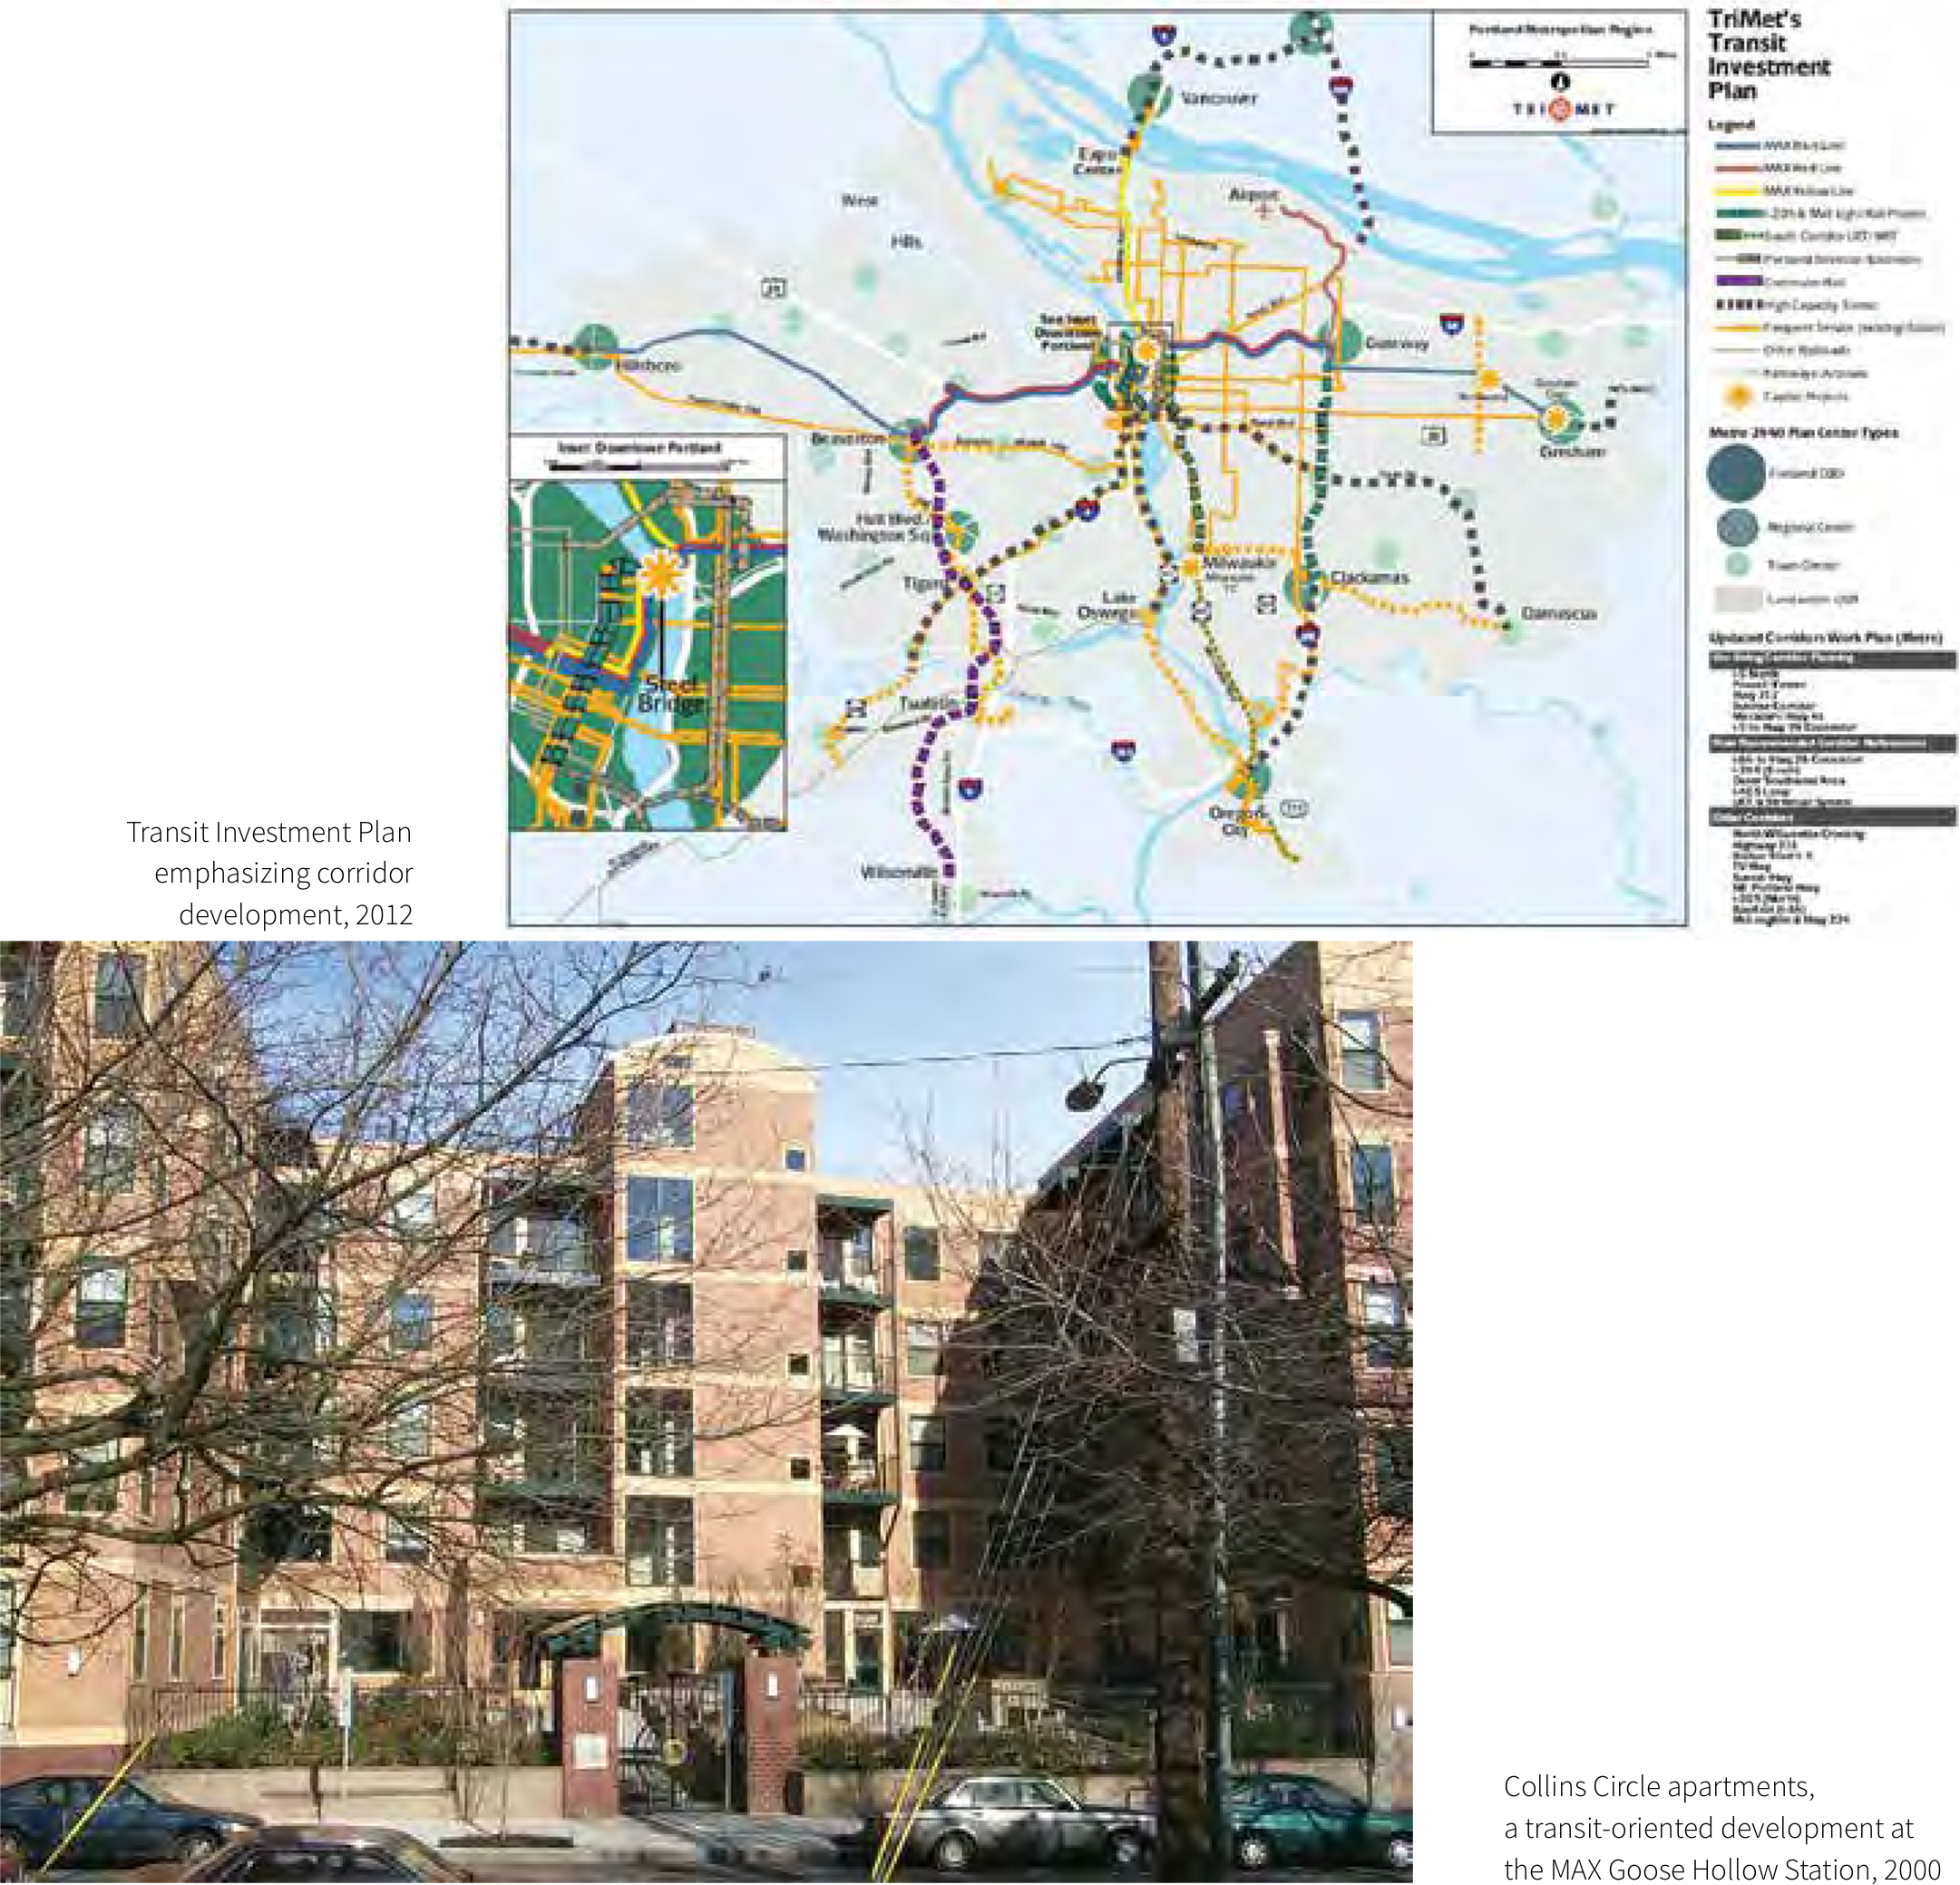
\includegraphics[width=0.9\linewidth]{img/trimet2015a_01}
		\label{fig:todtrimet}
		\legend{Fonte: adaptado de \citeonline[p. 68]{trimet2019a}}
	\end{figure}

	O papel da \gls{ugb} pode ser resumido da seguinte maneira, conforme \cite{metro2019a}:

	\begin{itemize}
		\item O solo dentro da \gls{ugb} suporta serviços urbanos. Exemplos: ruas; sistemas de água e esgoto; parques; escolas; proteção policiais e de bombeiros;
		\item A \gls{ugb} é uma das ferramentas para proteger fazendas e florestas do espraiamento urbano e promover um uso eficiente do solo, infraestrutura pública e serviços que estão dentro dela;
		\item O Metro Council faz a revisão do estoque de terra e publica o \textit{Urban Growth Report} (Relatório de Crescimento Urbano, em tradução livre), além de projetar o crescimento populacional e da oferta de emprego pelos próximos 20 anos. Se necessário, ajusta os limites da \gls{ugb} para que ela comporte o crescimento previsto;
		\item Os limites já foram alterados 36 vezes e, a partir de 2007, um sistema de reservas urbanas e rurais foi estabelecido.
	\end{itemize}
	
	O caso de Portland, contudo, está longe de ser trivial e facilmente replicável:
	
	\begin{citacao}
		``[\dots] o caso de Portland/Oregon, como uma autoridade metropolitana eleita e com atribuições importantes nas áreas de transporte e a organização de uso e ocupação do solo, \textbf{talvez seja uma das exceções mais notáveis} à regra de um sistema relativamente fragmentado com um conjunto grande de atores locais dispersos [\dots]'' \cite[p. 224]{klink2009a}
	\end{citacao}

	Ainda assim, Portland une transporte sobre trilhos, controle do urbano e preservação rural, sendo estudada mundialmente por seu planejamento urbano, como apontado por \citeonline{noronha2015a}:
	
	\begin{citacao}
		``Portland-OR é estudada por autores de vários locais do mundo por seu planejamento urbano, baseado no controle do perímetro aliado à preservação das áreas rurais e redução da expansão urbana desenfreada (JUN, 2008). O diferencial de Portland-OR é o veículo leve sobre trilhos (VLT), categorizado como railmax como principal meio de deslocamento entre os habitantes locais. Além do railmax, Portland-OR também oferece faixas próprias para incentivo do uso de bicicletas e até outros modos menos convencionais como o skate, já que é uma metrópole essencialmente universitária e por isso abriga muitos jovens que fazem uso destes modos de deslocamento.'' \cite[p. 17]{noronha2015a}
	\end{citacao}
	
	%===============================================================================
	%
	
	% ----------------------------------------------------------
	% ----------------------------------------------------------
	\postextual
	
	
	
	% informa o arquivo com a bibliografia. Deve ser o mesmo nome
	% (sem o sufixo) que será informado no ambiente filecontents
	% que está no final deste arquivo. Neste exemplo foi usado 
	% bibitemp.bib e bibtemp. Este comando insere a bibliografia
	% nesta posição (antes dos apêndices, anexos, índice remissivo)
	\bibliography{fontes}
	% ----------------------------------------------------------
	% Glossário
	% ----------------------------------------------------------
	% Consultar manual da classe abntex2 para orientações sobre o
	% uso do glossário.
	\renewcommand{\glossaryname}{Glossário}
	%\renewcommand{\glossarypreamble}{Esta é a descrição do glossário.\\ \\}
	\renewcommand*{\glsseeformat}[3][\seename]{\textit{#1}
		\glsseelist{#2}}
	
	% ---
	% Traduções para o ambiente glossaries
	% ---
	\providetranslation{Glossary}{Glossário}
	\providetranslation{Acronyms}{Siglas}
	\providetranslation{Notation (glossaries)}{Notação}
	\providetranslation{Description (glossaries)}{Descrição}
	\providetranslation{Symbol (glossaries)}{Símbolo}
	\providetranslation{Page List (glossaries)}{Lista de Páginas}
	\providetranslation{Symbols (glossaries)}{Símbolos}
	\providetranslation{Numbers (glossaries)}{Números} 
	% ---
	
	% ---
	% Imprime o glossário
	% ---
	\cleardoublepage
	\phantomsection
	\addcontentsline{toc}{chapter}{\glossaryname}
	% \glossarystyle{index}
	% \glossarystyle{altlisthypergroup}
	\glossarystyle{tree}
	\printglossaries
	% ---
	
	% ----------------------------------------------------------
	% Apêndices
	% ----------------------------------------------------------
	
	% ---
	% Inicia os apêndices. Não esquecer de fechar ao final de
	% cada um dos apêndices (\end{apendicesenv})
	% ---
	\begin{apendicesenv}
	
	% Imprime uma página indicando o início dos apêndices
	\partapendices
	
	% ----------------------------------------------------------
	\chapter{Jupyter Notebook} \label{ap:jupyter}
	% ----------------------------------------------------------
	
	Este apêndice transcreve integralmente o arquivo utilizado para geração do modelo de agrupamento por similaridade (vide \autoref{sec:machine}).
	
	\lstinputlisting[language=Python]{../modelo/notebook_clusters_sem_blob.ipynb}
	
	% ----------------------------------------------------------
	\chapter{Minuta de lei}
	% ----------------------------------------------------------
	
	Esta é a minuta de lei elaborada com base no Prognóstico (\autoref{sec:prognostico}).
	
	\end{apendicesenv}
	% ---
	
	
	% ----------------------------------------------------------
	% Anexos
	% ----------------------------------------------------------
	
	% ---
	% Inicia os anexos
	% ---
	%\begin{anexosenv}
	
	% Imprime uma página indicando o início dos anexos
	%\partanexos
	
	% ---
	%\chapter{Anexo I}
	% ---
	%Os anexos são similares aos apêndices se distinguindo pelo fato
	%que os apêndices são de autoria do autor da monografia e os 
	%anexos não são da autoria do autor da monografia.  Por exemplo,
	%se incluir no trabalho um modelo de um formulário preenchido
	%por alunos participantes de uma pesquisa, este será um apêndice
	%se o formulário foi criado pelo autor da monografia e será um
	%anexo se o formulário tiver sido criado por outros (por exemplo,
	%é um formulário padrão da escola em que o aluno que o preenche
	%estuda).
	%
	%Mesmo que o formulário tenha sido elaborado pela escola, uma
	%reprodução do formulário preenchido por cada aluno na pesquisa
	%será incluído no apêndice pois envolve o trabalho do autor da
	%monografia ao distribuir, coletar e reproduzir as respostas.
	%
	%Este é um exemplo de inclusão de capítulos de anexos em uma 
	%monografia.  Cada anexo é tratado como se fosse um capítulo.
	%Os anexos devem ser iniciados pelo comando de ambiente
	%\textbackslash begin\{anexoenv\} e encerrados pelo comando 
	%\textbackslash end\{anexoenv\}.
	%
	%\end{anexosenv}
	% ---
	%---------------------------------------------------------------------
	%---------------------------------------------------------------------
	
	%\printindex
	
	% Por padrão são incluídas no trabalho somente as referências
	% citadas ao longo do texto. No comando abaixo foram acrescentadas
	% algumas referências não citadas (neste texto servem apenas como
	% exemplos). Não deve ser usado o comando (mais simples) 
	% \nocite{*}, pois este parece não ser compatível com o
	% abntex2cite
	%\nocite{abntex2cite,abntex2wiki,boyer,eves,iezzi,kletenic,
	%        diomara,steinbruch,intusolatex,feynman,shannon,
	%        luisfelipe,turing}
\end{document}
